% Load the kaobook class
\documentclass[
    a4paper, % Page size
    fontsize=10pt, % Base font size
    twoside=true, % Use different layouts for even and odd pages (in particular, if twoside=true, the margin column will be always on the outside)
    %open=any, % If twoside=true, uncomment this to force new chapters to start on any page, not only on right (odd) pages
    %chapterentrydots=true, % Uncomment to output dots from the chapter name to the page number in the table of contents
    numbers=noenddot, % Comment to output dots after chapter numbers; the most common values for this option are: enddot, noenddot and auto (see the KOMAScript documentation for an in-depth explanation)
    fontmethod=tex,
]{kaobook}

\ifxetexorluatex
    \usepackage{polyglossia}
    \setmainlanguage{english}
\else
    \usepackage[english]{babel}
\fi
\usepackage[english=american]{csquotes}
\setcounter{tocdepth}{1}
\usepackage{orcidlink}
\usepackage{siunitx}
\usepackage{astro}

\usepackage[backend=biber, style=numeric-comp,backref, sorting=none, firstinits=true,maxnames=2]{biblatex}

% Hack to include Collaboration author field
\DeclareSourcemap{
 \maps[datatype=bibtex,overwrite=true]{
  \map{
    \step[fieldsource=Collaboration, final=true]
    \step[fieldset=usera, origfieldval, final=true]
  }
 }
}

\renewbibmacro*{author}{%
  \iffieldundef{usera}{%
    \printnames{author}%
  }{%
    \printfield{usera}, \printnames{author}%
  }%
}%

\usepackage{kaobiblio}
\addbibresource{thesis.bib}

\usepackage[framed=true]{kaotheorems}
\usepackage{kaorefs}

\graphicspath{{figures/}{images/}}

\makeindex[columns=3, title=Alphabetical Index, intoc]


\begin{document}

%----------------------------------------------------------------------------------------
%   BOOK INFORMATION
%----------------------------------------------------------------------------------------
\subject{Doctoral Thesis}
% \titlehead{Optical Follow-Up of High-Energy Neutrinos}
\title[Optical Follow-Up of High-Energy Neutrinos]{Optical Follow-Up of High-Energy Neutrinos}
\author[SR]{Simeon Reusch}% \orcidlink{0000-0002-7788-628X}}
\date{\today}
\publishers{Humboldt-Universität zu Berlin}

%----------------------------------------------------------------------------------------

\frontmatter

\makeatletter 
\uppertitleback{\@titlehead}

\lowertitleback{
    \textbf{Copyright} \\
    \cczero\ This book is released into the public domain using the CC0 code. To the extent possible under law, I waive all copyright and related or neighbouring rights to this work. To view a copy of the CC0 code, visit: \\\url{http://creativecommons.org/publicdomain/zero/1.0}
    
    \medskip
 
    This thesis was typeset with the help of \href{https://sourceforge.net/projects/koma-script}{\KOMAScript} and \href{https://www.latex-project.org}{\LaTeX} using the \href{https://github.com/fmarotta/kaobook}{kaobook} class.
    
    \medskip

    The code used to typeset this thesis and create the figures within can be accessed at \href{https://github.com/simeonreusch/koma-thesis}{github.com/simeonreusch/thesis}

    \medskip
    
    \textbf{Publisher} \\
    First published in August 2023 by \@publishers
}
\makeatother


\maketitle

\begingroup % Local scope for the following commands

% Define the style for the TOC, LOF, and LOT
%\setstretch{1} % Uncomment to modify line spacing in the ToC
%\hypersetup{linkcolor=blue} % Uncomment to set the colour of links in the ToC
\setlength{\textheight}{230\vscale} % Manually adjust the height of the ToC pages

% Turn on compatibility mode for the etoc package
%\etocstandarddisplaystyle % "toc display" as if etoc was not loaded
%\etocstandardlines % "toc lines as if etoc was not loaded

\tableofcontents
\listoffigures

\let\cleardoublepage\bigskip
\let\clearpage\bigskip

\listoftables

\endgroup

\mainmatter
\setchapterstyle{kao}

%\chapter{Theoretical background}
%\addpart{Title of the Part}
\pagelayout{margin}


% \setchapterimage[7cm]{theory/AT2019dsg_cropped.jpg}
\chapter{Neutrino Astronomy}\label{theory}
\labch{neutrino_astronomy}

Contrary\marginnote{Artistic impression of a tidal disruption event. Material from the shredded star starts accreting around a black hole, and a jet is launched. Image Credit: DESY and Science Communication Lab.} to photons---especially optical ones---neutrinos are extremely hard to detect. This explains why neutrino astronomy is such a recent development. As this thesis is concerned with the identification of the astrophysical sources of high-energy neutrinos, this chapter will first detail what neutrinos are, and then explain how high-energy neutrino astronomy has advanced. This will be followed by a discussion of different types of proposed source classes of high-energy neutrinos. Lastly, established counterparts to neutrinos will be discussed, as well as upper limits on most of the proposed source classes.

\section{Neutrinos}
Neutrinos were first predicted by Pauli in the 1930s~\sidecite{Giunti2007}, given firm theoretical footing by Fermi in 1934~\sidecite{Fermi1934}, and experimentally detected by Reines and Cowan in 1955~\sidecite{Reines1956}.

\subsection{The Neutrino Hypothesis}\label{neutrino_hypothesis}

\begin{marginfigure}
    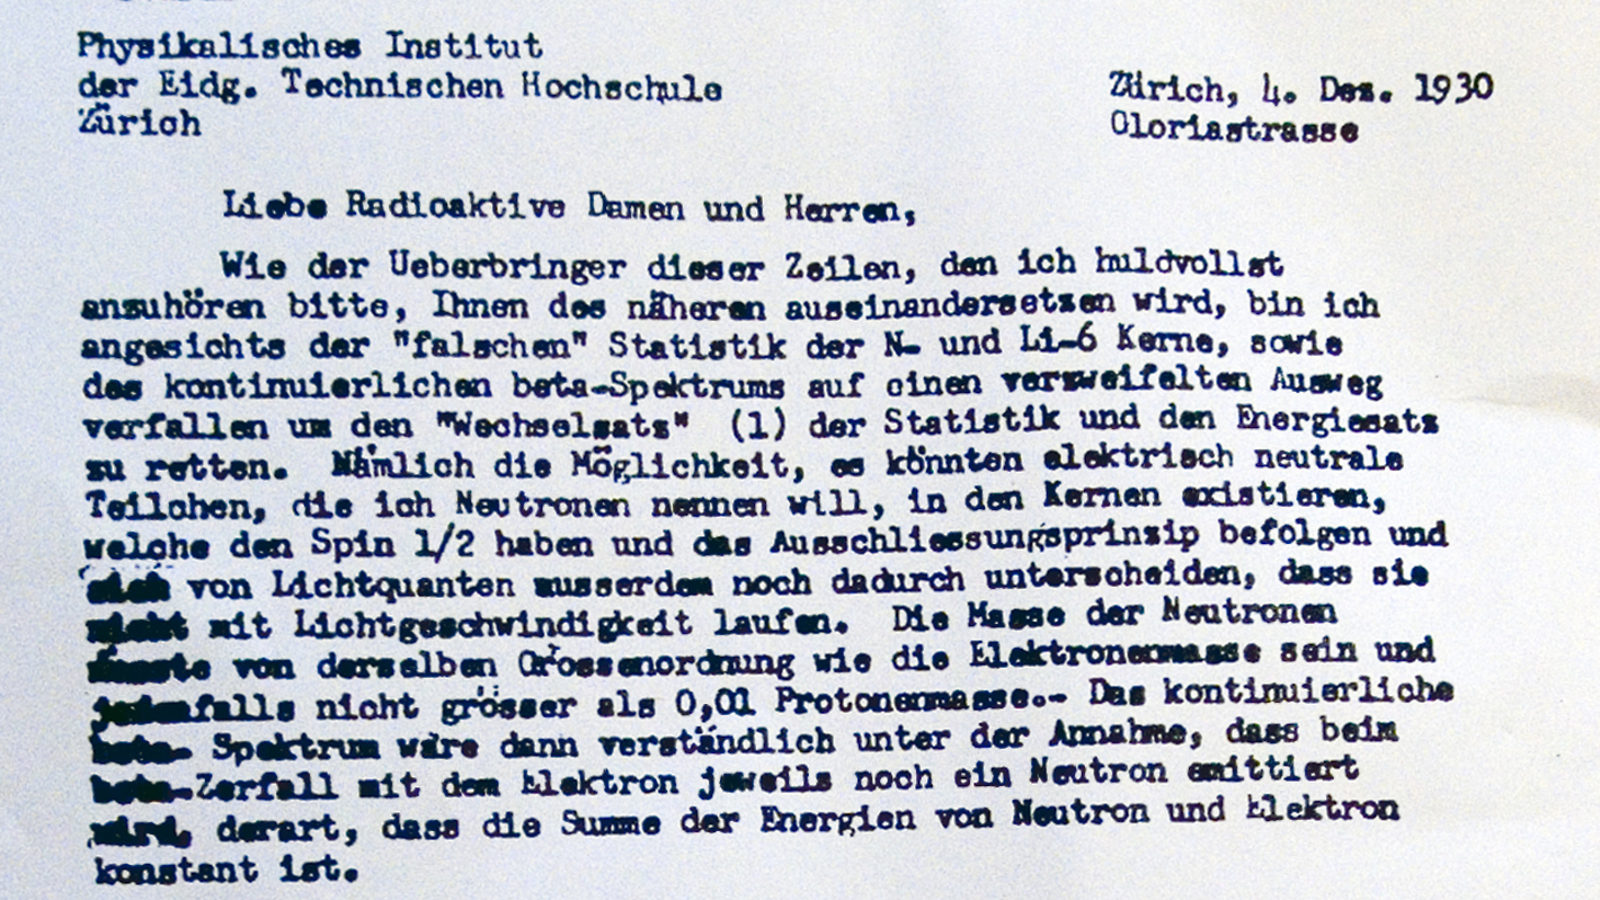
\includegraphics{theory/pauli_neutrino.jpg}
    \caption[Pauli's letter proposing the neutrino]{Pauli's open letter from December 1930, proposing the existence of the neutrino (he called it `neutron' at the time) to the community. Image credit: Pauli Letter Collection, CERN.}
    \labfig{pauli_letter}
\end{marginfigure}

Wolfgang Pauli reluctantly proposed the neutrino to explain the continuous $\beta$-spectrum of decaying uranium. When nuclear elements decay, they emit different particles. Different types of emission were dubbed $\alpha$-, $\beta$- and $\gamma$ radiation~\sidecite{Rutherford1899,Villard1900}; the first being helium-4 nuclei, the second electrons or protons, and lastly energetic photons. Contrary to $\alpha$- and $\gamma$-radiation, the spectrum of $\beta$-radiation turned out to be continuous, while one would expect discrete energy levels for the emitted particles.

In $\beta^-$-decay, the nucleus of an atom emits an electron when undergoing the nuclear transition $(A,Z)\rightarrow(A,Z+1) + e^-$. Here, $A$ is the mass number (the number of nucleons in the atom), and $Z$ is the atomic number (the number of protons in the nucleus)---a neutron-proton conversion occurs, as is known nowadays. In this scenario, the decay is a two body problem, involving the nucleus and an electron. When converting a neutron into a proton, the resulting binding energy of the atom is lower, and this energy needs to be accounted for. Also, the positive charge gained by the nucleus during the transition must be equalized somewhere.

Therefore, the emitted electron carries the quantized energy lost to the atom due to its transition to the final state. As was already known at that time, this tight distribution of energy is fixed by the difference in binding energy, so one would expect a narrow energy spectrum for the emitted electron, similar to $\alpha$- and $\gamma$-radiation. But the observed electron spectrum was continuous, hence the puzzlement of the community. Bohr proposed loosening the requirement of energy conservation---a suggestion Pauli was strongly opposed to\sidenote{He brought forth a though experiment of a closed box, within which $\beta$-decay happens. The weight of this box would change over time, a result he deemed paradoxical.}~\sidecite{Jensen2000}.

Pauli instead took refuge in what he considered a desperate solution, and suggested that the $\beta$-decay was in fact a three body problem, with a neutral particle carrying a variable fraction of the released energy~\sidecite{Bilenky2012}. This would explain the continuous electron spectrum. He also assumed that the hypothetical second particle interacted extremely rarely, which explains why it had not yet been observed.

The next advancement in the understanding of the neutrino was due to Enrico Fermi in 1934. By then, the picture of the atomic nucleus had been complemented by the neutron, discovered by James Chadwick two years earlier. Fermi developed the first theory of $\beta$-decay, analogous to the description of the emission of photons from excited nuclei~\cite{Fermi1934}. He assumed that the electron-neutrino pair is produced when a neutron within the nucleus transitions into a proton: $n \rightarrow p + e^- + \bar{\nu}$. The predictions from his theory were in fair agreement with observations, provided the neutrino mass was quite small~\cite{Fermi1934}.

\subsection{Neutrino Detections}
It took another 22 years until the neutrino was discovered experimentally. In the meantime, the nuclear bomb had been conceived, proposed, built, and dropped twice. The Savannah River Plant nuclear reactors were constructed as part of the nuclear arms race effort to develop more fission bombs, producing plutonium and tritium. On a more pacifistic note, Reines and Cowan used the hypothesized flux of neutrinos from the reactors to first experimentally detect a neutrino~\cite{Reines1956} (with a confirmation in~\sidecite{Cowan1956}).

The experiment was based on the inverse beta decay, in which the predicted neutrino (in fact, an electron antineutrino) reacts with a proton, converting it into a neutron and releasing a positron ($\bar{\nu_e} + p \rightarrow n + e^+$). The released positron then annihilates with a free electron within the target material (for this they used $\text{H}_2\text{O} + \text{CdCl}_2$). In this process, two \SI{511}{\kilo\eV} photons are released, emitted in opposite directions due to conservation of momentum. These photons are then detected by a liquid scintillator surrounding the target. The neutron diffuses through the target medium for a while until it is finally captured by the cadmium, emitting a delayed photon signal (see Fig.~\ref{fig:neutrino_discovery}).

\begin{figure}[htb]
    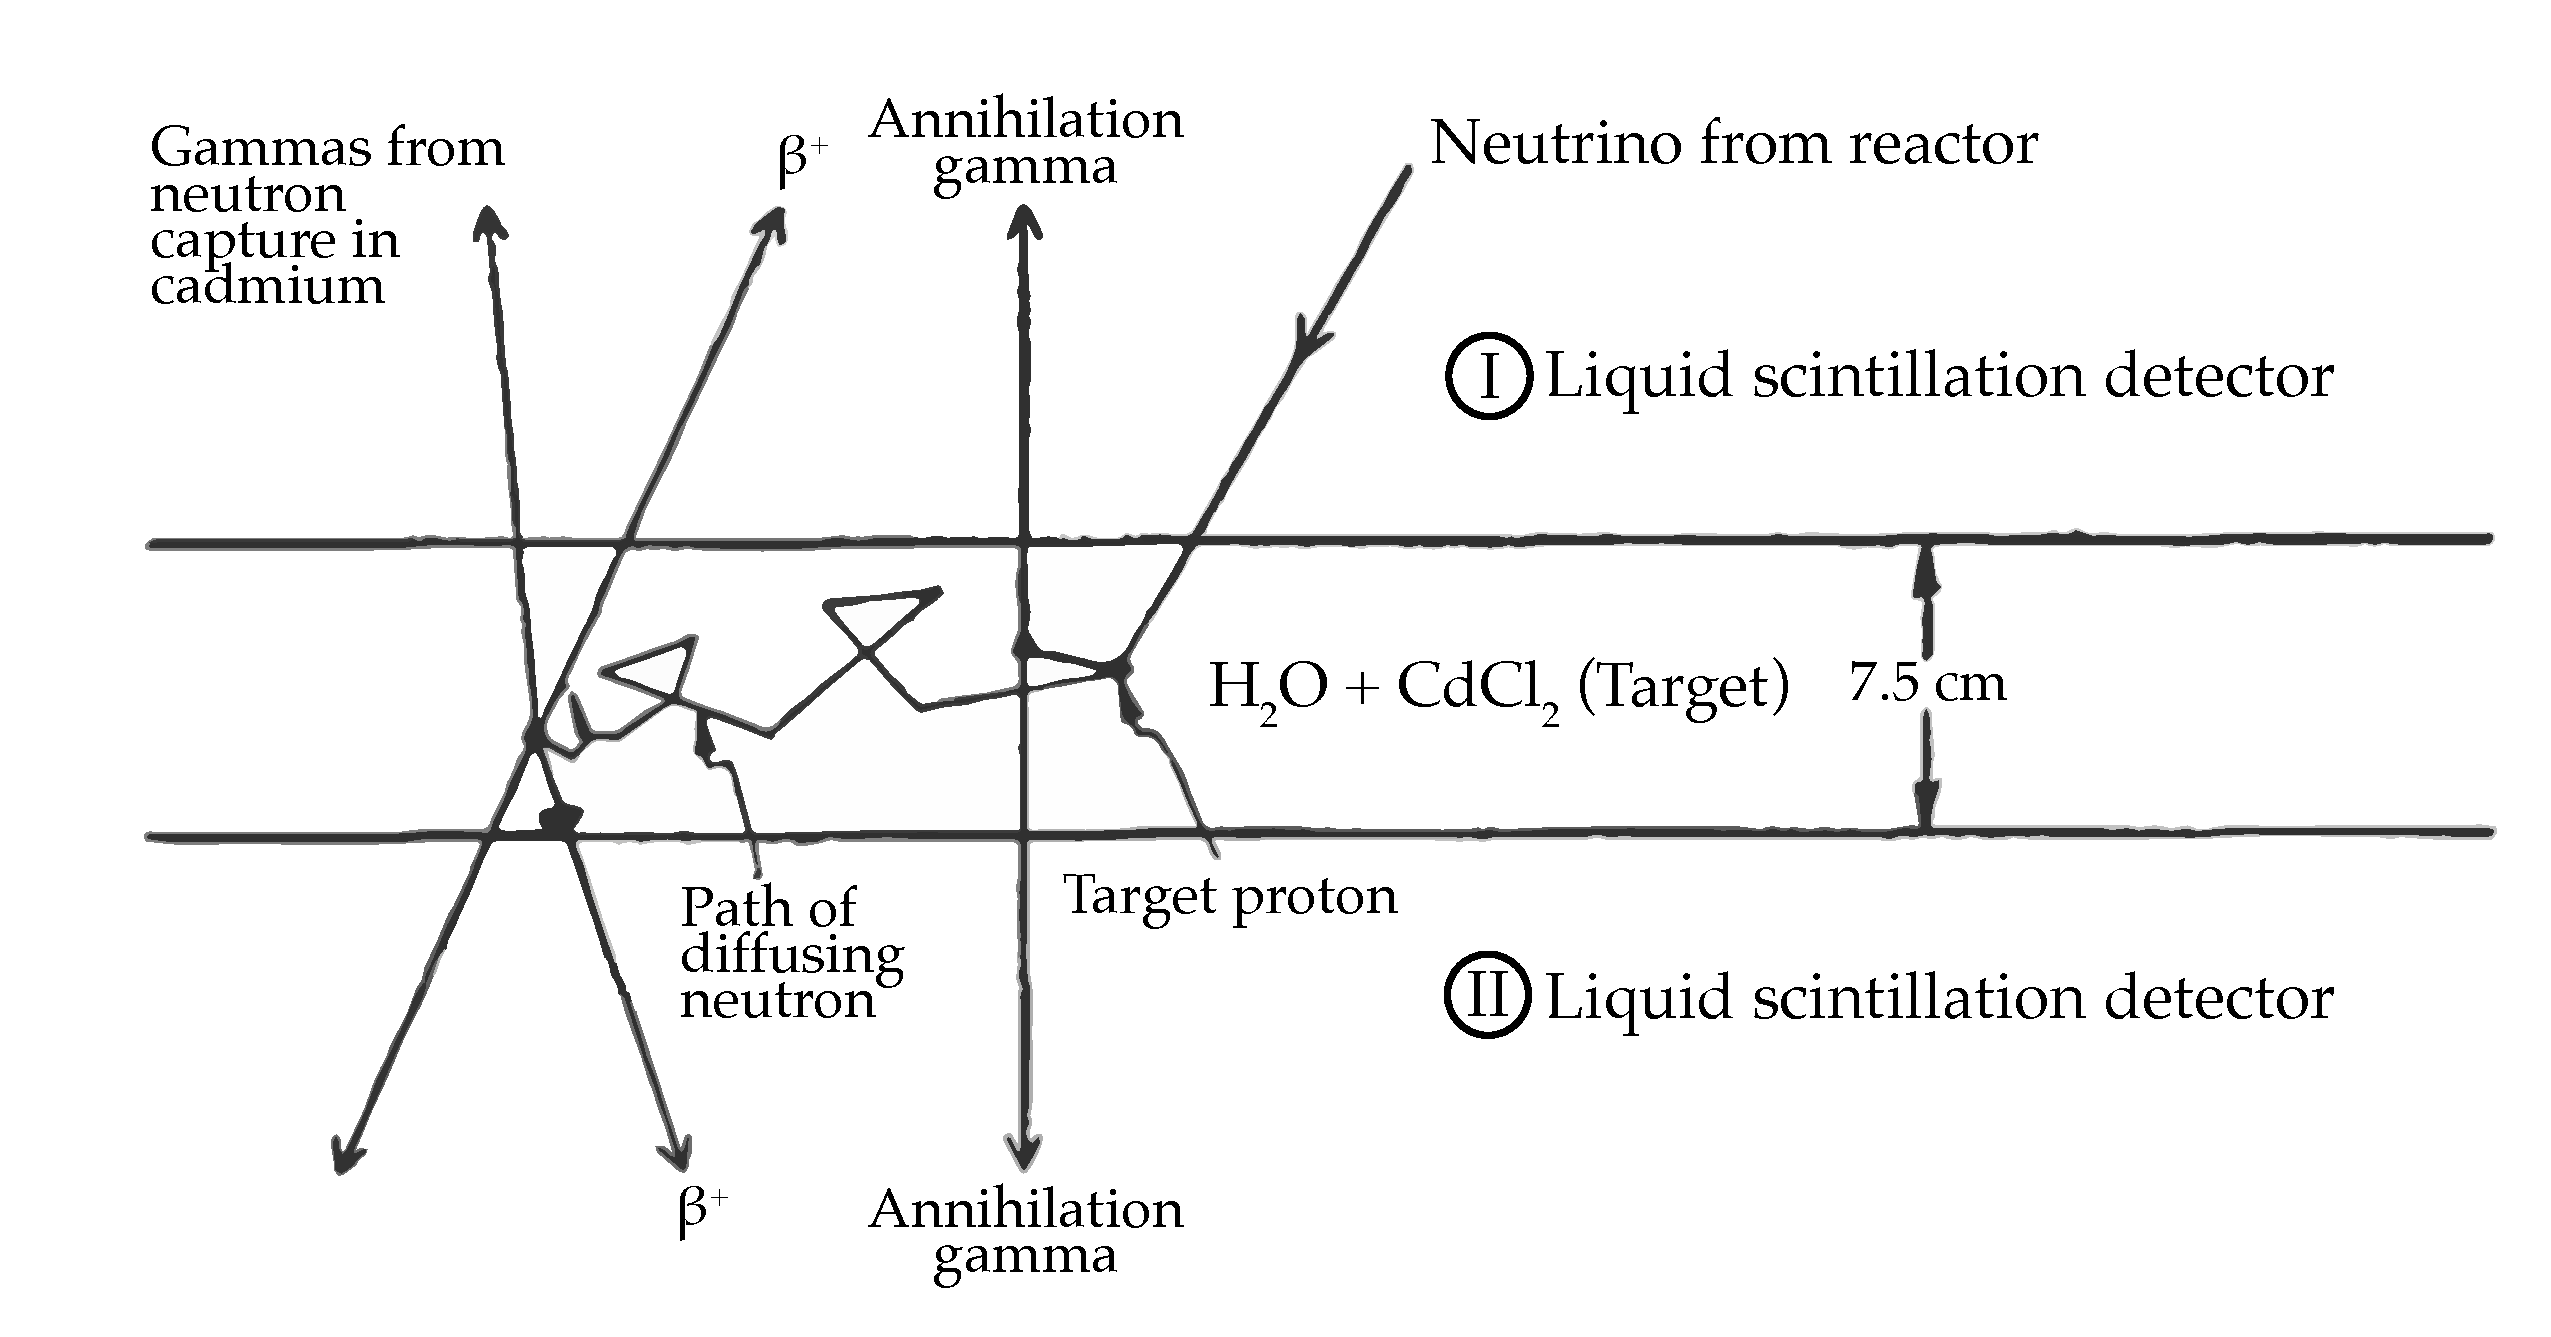
\includegraphics[width=0.8\textwidth]{theory/neutrino_discovery_principle.pdf}
    \caption[Neutrino discovery schematic]{Experimental setup for the discovery of the neutrino. Adapted from~\cite{Reines1956}.}
    \labfig{neutrino_discovery}
\end{figure}

The extremely low interaction rate, or, in other words, the small interaction cross-section of the neutrino, required large amounts of target material and liquid scintillator to detect this reaction~\cite{Giunti2007}. Ultimately, thanks to the unique event signature described above, Reins and Cowan succeeded, reporting a neutrino detection rate of $2.88^{+0.22}_{-0.22}$\,\si{\ct\per\hour}~\cite{Reines1956}.

\subsection{Discovery of the Muon Neutrino}
Another important step was the discovery of the muon neutrino: At the Brookhaven National Lab in the US, muons and kaons from an accelerator were used to prove the existence of this neutrino flavor. Prior to the experiment, it had already been pointed out by Lee and Yang that the experimental failure to detect the decay $\mu \rightarrow e \gamma$ strongly hinted at the existence of a muon neutrino. This decay is only allowed if there is no difference between $\nu_e$ and $\nu_\mu$~\sidecite{Ekspong1993}.

The goal of the Brookhaven experiment~\sidecite{Danby1962} was to directly detect the muon neutrino by producing $\pi^+$ through bombarding a Beryllium target with \SI{15}{\giga\eV} protons. $\pi^+$ primarily decay to $\mu^+ + \nu_\mu$, as the channel $\pi^+ \rightarrow e^+ + \nu_e$ is strongly suppressed, see~\cite{Bilenky2012}. In a subsequent decay channel, almost all $\mu^+$ decay, only allowing the muon neutrinos to pass. These were directed towards a neutrino detector, consisting of aluminum plates located in a spark chamber. The neutrinos would interact with the aluminum nuclei and produce charged leptons. If there was no difference between $\nu_\mu$ and $\nu_e$, one would expect detecting $e^-$ and $\mu^-$ in equal numbers. However, the experiment observed a significant number of muons (29) and detected only a few electrons (6). The electrons could be attributed to background noise, therefore the experiment proved the existence of the muon neutrino~\cite{Danby1962}.

\subsection{The Solar Neutrino Problem}

\begin{marginfigure}[-0.8cm]
    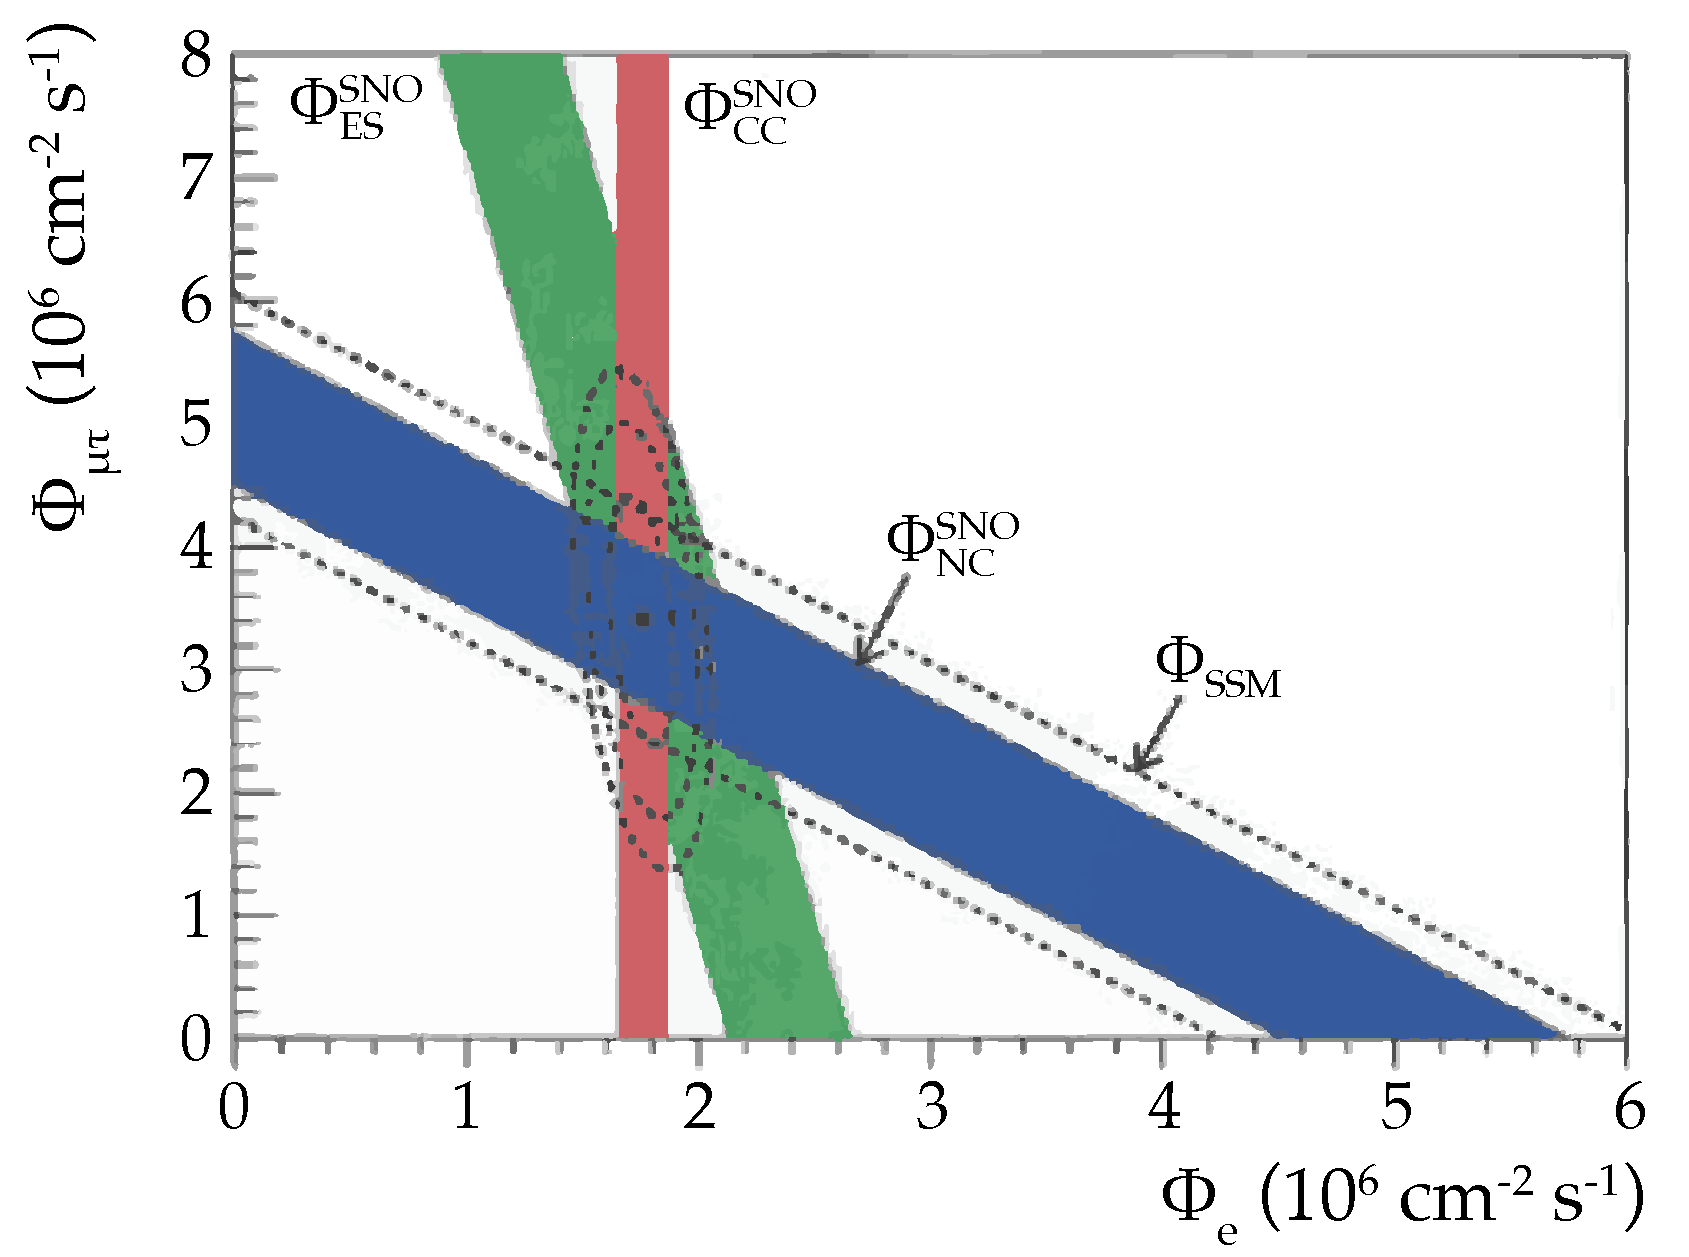
\includegraphics{theory/sno_flux.pdf}
    \caption[Solar neutrino flux measured by SNO]{The solar neutrino flux as measured by SNO\@. The x-axis shows the $\nu_e$ flux, while the y-axis shows the flux of solar $\nu_\mu$ and $\nu_\tau$. The intersection point shows the best-fit flux values for $\nu_e$ and $\nu_{\mu,\tau}$, with a resulting flavor ratio of $\sim1/3$ for all types. Adapted from~\cite{Ahmad2002}.}
    \labfig{sno_flux}
\end{marginfigure}

The neutrino was had been detected. This, combined with the prediction that the process of nuclear fission within the Sun should release neutrinos, triggered the hunt for solar neutrinos. The Sun creates neutrinos both via the $pp$ chain and the CNO cycle, in both processes converting four protons and two electrons into a $^4\text{He}$ nucleus and two electron neutrinos: $4p + 2e^- \rightarrow  ~^4\text{He} + 2\nu_e + \SI{26.7}{\mega\eV}$. The excess energy is then released via photons or neutrinos carrying kinetic energy~\cite{Giunti2007}.

Solar electron neutrinos were first detected in the 1960s in the Homestake experiment by Davis. He operated a tank located underground in the Homestake mine in South Dakota in the US, filled with \SI{380}{\meter\cubed} of tetrachloroethene. This allowed antineutrino capture via the inverse beta decay $\nu_e +~ ^{37}\text{Cl} \rightarrow ~ ^{37}\text{Ar} + e^-$, transmuting chlorine to argon. First results after 150 days of data taking resulted in an upper neutrino flux limit much lower than the theoretical expectations~\sidecite{Davis1968}. The experiment would run continuously from 1970 to 1994, detecting a neutrino flux that never exceeded \SI{50}{\percent} of the expected flux. The fact that the measured flux was consistently lower than the predicted one, despite various checks and improvements, became known as the solar neutrino problem~\sidecite{Bahcall1976}.

A solution to the solar neutrino problem was first proposed by Gribov and Pontecorvo in 1969~\sidecite{Gribov1969}: The missing electron neutrinos from the Sun could have oscillated into neutrinos of a different flavor while traveling to Earth. This proposed neutrino oscillation was observed by the Sudbury Neutrino Observatory (SNO) in 2002; while evidence for the oscillation of atmospheric neutrinos had already been brought forth four years earlier by the Super-Kamiokande detector~\sidecite{Fukuda1998}. The SNO detector was sensitive to two types of interactions: One channel in which only $\nu_e$ could participate, and one open to neutrinos of all flavors. It was determined that the flux of solar $\nu_e$ was $\frac{1}{3}$ of the total neutrino flux (consisting of $\nu_e$, $\nu_\mu$ and $\nu_\tau$\sidenote{The existence of the tau neutrino had been confirmed one year earlier by the Direct Observation of the Nu Tau (DONUT) experiment~\cite{Kodama2001}.}), see Fig.~\ref{fig:sno_flux}. This result was in full agreement with theoretical predictions for the solar neutrino flux, and directly showed that neutrinos do oscillate~\sidecite{Ahmad2002}.

These oscillations can be described by the $3\times3$ unitary transformation matrix known as the Pontecorvo-Maki-Nakagawa-Sakata (PMNS) matrix, that works analogous to the matrix describing the quark flavor mixing (Cabbibo-Kobayashi-Maskawa, or short CKM, matrix). The values of the matrix elements must be determined experimentally, as there is no underlying theory predicting them.

\subsection{Neutrino Mass}
By observing solar neutrino oscillations, the SNO experiment also established the fact that neutrinos have mass---contradicting the Standard Model model of particle physics. Only massive particles allow oscillation between flavor eigenstates and mass eigenstates~\sidecite{Fisher1999}. It therefore does not make sense to ask for the mass of e.g.\ an electron neutrino, as this flavor eigenstate is a superposition of different mass states. One can speak of the effective electron neutrino mass, though; this property is defined as

\begin{equation}\label{pmns}
    m_\nu = \sqrt{ \Sigma_i |U_{ei}|^2 m_i^2 },
\end{equation}

\begin{marginfigure}
    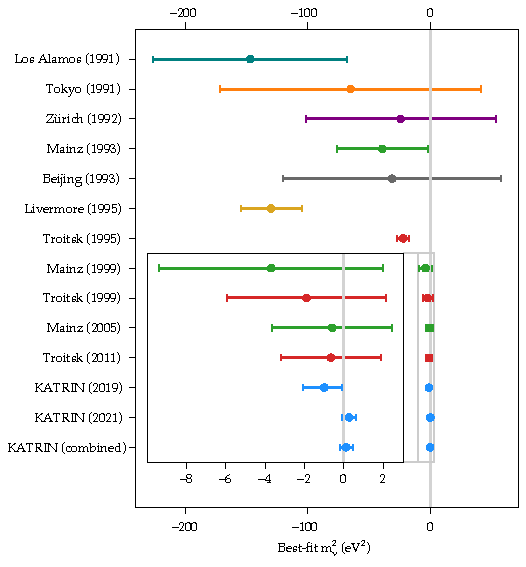
\includegraphics{theory/mass_history.pdf}
    \caption[Neutrino mass upper limit history]{The history of upper limits on the neutrino mass. From~\cite{Aker2022}.}
    \labfig{mass_history}
\end{marginfigure}

where $U$ is the PMNS matrix describing the neutrino state mixing, i.e.\ a collection of nine experimentally determined values. If one could take individual mass measurements of the electron neutrino, one would measure the mass $m_i$ with probability $|U_{ei}|^2$.

Neutrino oscillations are only sensitive to the squared mass differences between the three mass states, as there is no zero point in Eq.~\ref{pmns}. One way to measure the average proper neutrino mass is the close inspection of the beta-decay spectrum (see Section~\ref{neutrino_hypothesis}). The most recent in a long line of experiments to determine neutrino masses (see Fig.~\ref{fig:mass_history}) is the Karlsruhe Tritium Neutrino Experiment (KATRIN). It uses the beta decay of tritium. If the neutrino is massless, the energy spectrum of the emitted electron will extend up to the total energy released in the decay (\SI{18.6}{\eV}). On the other hand, if the neutrino mass is non-zero, the electron spectrum will always be short of that amount of energy. Note that in principle one could obtain all three neutrino masses from such an experiment if it weren't for current technological limitations. The latest upper limit from KATRIN on the effective electron antineutrino mass is $m_\nu < \SI{0.8}{\eV}$ at the \SI{90}{\percent} confidence level~\sidecite{Aker2022}.


\subsection{Current Understanding}\label{neutrinos_current}
The Standard Model of particle physics knows three flavors of neutrinos, which are superposition of three mass states~\sidecite{Barger2012}. Their mass is small, but exists. Neutrinos have neither electromagnetic, nor color charge, but possess a weak hypercharge. This weak hypercharge lets them partake in weak interactions, which are mediated by exchanging $W$ or $Z$ bosons. Fig.~\ref{fig:neutrino_interactions} details some possible neutrino interaction channels, all constituting deep inelastic scattering with the quarks contained in nucleons. This is the dominant interaction mode for high-energy neutrinos with energies at or above several \unit{\giga\eV} in a medium.

\begin{figure}[htb]
    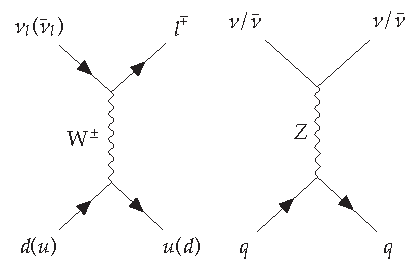
\includegraphics[width=0.55\textwidth]{theory/neutrino_interactions_feynman_short.pdf}
    \caption[Neutrino interactions]{Different neutrino interaction channels for deep inelastic scattering. Left: interaction of neutrinos (antineutrinos) with quarks by exchange of a $\text{W}^{\pm}$ boson. Right: interaction of neutrinos of all types by exchange of a Z boson. The interaction on the left is called Charged Current (CC) interaction, while the one on the left is dubbed Neutral Current (NC) interaction.}
    \labfig{neutrino_interactions}
\end{figure}

Interactions that involve electromagnetically charged $\text{W}^-$ bosons are called Charged Current (CC) interactions, while those involving neutral Z bosons are called Neutral Current (NC) interactions. For example, a neutron beta-decaying into a proton is a charged current interaction, as charge needs to be moved.

\begin{figure}[htb]
    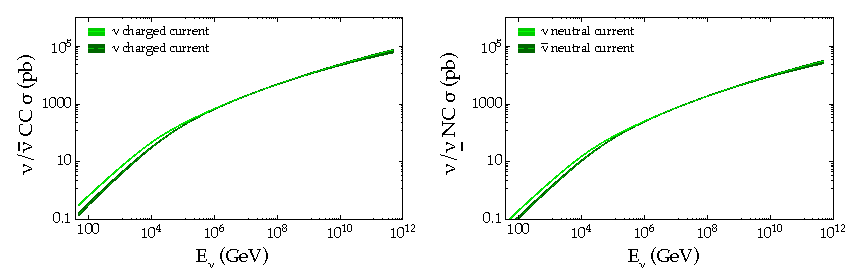
\includegraphics{theory/high_energy_nu_xsec.pdf}
    \caption[High-energy neutrino cross-section]{High-energy neutrino cross-section for interactions with matter equally composed of neutrons and protons. The unit on the y-axis are picobarn (\SI{e-40}{\m\squared}). The figure on the left shows charged-current interactions, while the one on the right displays neutral-current interactions, both for neutrinos and antineutrinos. Adapted from~\cite{CooperSarkar2011}.}
    \labfig{high_energy_nu_xsec}
\end{figure}

The cross-section for neutrinos with matter significantly increases with energy, as can be seen in Fig.~\ref{fig:high_energy_nu_xsec}. This is helpful for the detection of high-energy neutrinos, as this effect at least partially counterbalances the probable decrease in numbers of neutrinos produced in cosmic sources towards higher energies. On the other hand, neutrino detectors like IceCube are increasingly insensitive to neutrinos of the highest energies that sometimes have to traverse the Earth's core and get absorbed along the way.

\pagebreak

For a better understanding of neutrino astronomy, it is beneficial to broadly divide the subject into two main categories, as the processes and instruments involved are fairly different: low-energy and high-energy neutrino astronomy. As high-energy neutrino astronomy is intertwined with cosmic-ray astrophysics, a discussion of cosmic rays will be interspersed.

\section{Low-Energy Neutrino Astronomy}
Low-energy neutrinos, i.e.\ those carrying energies up to $\mathcal{O}(\unit{\mega\eV})$, are produced in stellar fusion processes and in supernovae. The primary stellar fusion process we can study is of course the Sun.

\subsection{Stellar Neutrinos}
\begin{marginfigure}
    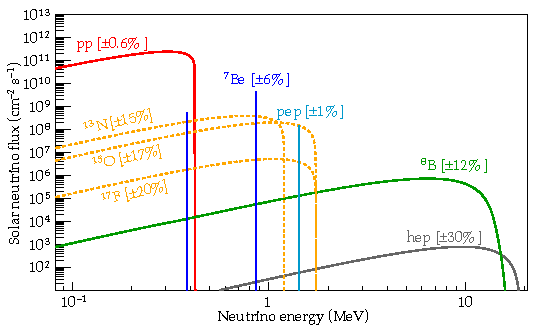
\includegraphics{theory/solar_neutrinos.pdf}
    \caption[Predicted solar neutrino flux]{Predicted solar neutrino flux. From~\cite{Agostini2018}.}
    \labfig{solar_neutrino_flux}
\end{marginfigure}

As briefly mentioned above, the solar neutrinos stem from two processes: The $pp$ chain and the CNO cycle. Within the $pp$ chain, neutrinos get produced by the proton-neutron conversion preceding the fusion of $p+n$ to $^2 \text{H}$. This conversion either happens via the $\beta^+$ decay $p \rightarrow n + e^+ + \nu_e$, resulting in a continuous neutrino spectrum (red curve in Fig.~\ref{fig:solar_neutrino_flux}), or via electron capture $e^- + p \rightarrow n + \nu_e$, which results in a line spectrum (leftmost blue line).

As one can see in Fig.~\ref{fig:solar_neutrino_flux}, the predicted solar neutrino spectrum is composed of different channels. Towards \unit{\mega\eV} energies, the solar neutrino flux is dominated by the decay of $^8\text{B}\rightarrow ~^8\text{Be} + e^+ + \nu_e$ (green curve) happening in one of the subsequent evolutions of the $pp$ chain. This particular process does not contribute much to the radiative energy output of the Sun, but it was the responsible mechanism for the solar neutrino flux, of which $\frac{2}{3}$ were missing, constituting the aforementioned solar neutrino puzzle.

Fig.~\ref{fig:solar_neutrino_flux} also shows that the predicted flux cuts off around \SI{\sim10}{\mega\eV}, so only low-energy neutrinos are expected from the Sun and similar stars.

\subsection{Supernovae}\label{sne}
Only with the first extragalactic neutrino source the era of neutrino astronomy truly began. This source was \emph{SN1987a}, an extremely close-by supernova in the Large Magellanic Cloud (LMC) that occurred in February 1987~\sidecite[-40pt]{Kunkel1987}.

Since Kepler's supernova almost 500 years ago---a Type Ia supernova (see below) that occurred in 1604 in the Milky Way---\emph{SN1987a} was the first supernova observable by the naked eye alone, sporting an impressive brightness of $3-4$ mag due to its proximity~\sidecite[-70pt]{Spurio2018}.\ \emph{SN1987a} was the core-collapse of \emph{Sanduleak-69202}, a blue supergiant, resulting in a Type IIP supernova\sidenote[][-70pt]{Though the rise instead of a plateau phase within its light curve gave it its own class, SN1987A-likes~\cite{Arcavi2017}.}~\sidecite[-38pt]{Utrobin2021}. After the optical detection of the source the neutrino detectors Kamiokande-II, Irvine-Michigan-Brookhaven (IMB) and the Baksan Neutrino Observatory (BNO) measured a burst of neutrinos predating the light from the supernova by 3 hours~\sidecite[-35pt]{Hirata1987,Bionta1987}, see also Fig.~\ref{fig:sn1987a_flux}.

In total, 25 neutrinos were detected by the three instruments (had IceCube already been operational in 1987, it should have detected \num{\sim13000} neutrinos~\sidecite{Halzen2017}). These rates were in agreement with theoretical models for core-collapse supernovae, assuming that \SI{99}{\percent} of the supernova energy is released in the form of neutrinos of all flavors.

\begin{marginfigure}
    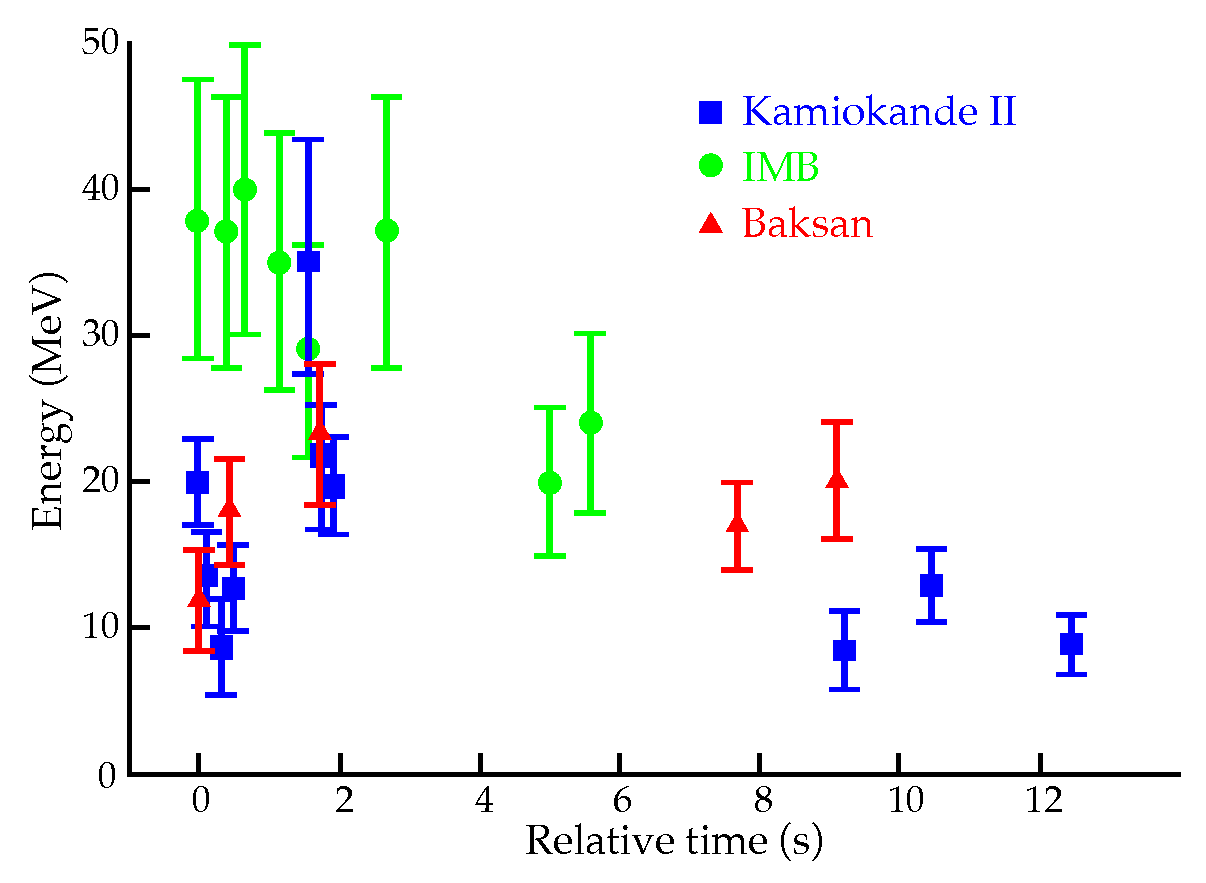
\includegraphics{theory/sn1987a_flux.pdf}
    \caption[Neutrinos from \emph{SN1987a}]{The neutrinos from \emph{SN1987a}, as measured by Kamiokande-II, IMB and BNO (Baksan). Figure\ adapted from~\cite{Grupen2005}.}
    \labfig{sn1987a_flux}
\end{marginfigure}

Historically, supernovae have been classified according to the presence of lines in their spectra. SNe of Type I lack hydrogen lines, in contrast to Type II SNe which do show hydrogen lines. Non-hydrogen SNe are further subdivided into SNe Ia that display both silicon and helium lines, SNe Ib that lack the silicon lines, and SNe Ic that contain neither silicon nor helium lines in their spectra.

\subsubsection{SNe Ia}\label{sne_ia}
SNe Ia constitute a class sui generis. The underlying physical scenario for their explosion is often assumed to be a white dwarf accreting matter from a companion star, the so-called Single Degenerate (SD) scenario. The accretion eventually causes the star's mass to exceed the Chandrasekhar limit of $\sim1.4~M_\odot$. At this point the gravitational force overcomes the electron degeneracy pressure, and the star begins to burn carbon due to the increased pressure. Soon after that, a runaway thermonuclear reaction starts, and the white dwarf blows up violently~\sidecite{Iben1984}.

A second possible scenario that has recently gained traction is the Double Degenerate (DD) scenario. In this model, the SN Ia is the result of two gravitationally bound white dwarfs (a binary system) shedding gravitational energy in the form of gravitational waves and thereby slowly closing in on each other. Ultimately, they merge and cause the supernova explosion~\cite{Iben1984}.

In either scenario (see~\sidecite{Maoz2014} for a review), the luminosity of the resulting explosion can be standardized using the Philips relation~\sidecite{Phillips1993}. This makes SNe Ia standard candles, excellent instruments to measure cosmological distances. As they are mainly powered by the decay $^{56}\text{Ni}~\rightarrow~^{56}\text{Co}~\rightarrow~^{56}\text{Fe}$, they are expected to produce low-energy neutrinos, but not in large quantities when compared to core-collapse SNe (see next Section~\ref{ccsne})~\sidecite{Alsabti2017}.

\subsubsection{Core-Collapse Supernovae}\label{ccsne}

\begin{marginfigure}
    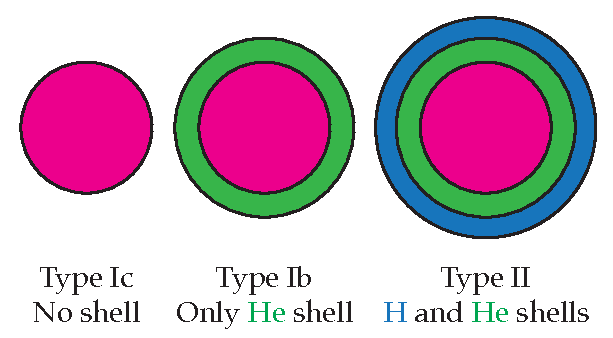
\includegraphics{theory/sn_shells.pdf}
    \caption[CCSN shells]{CCSN shells. The presence or absence of helium and hydrogen shells explains the differences in the respective spectra of CCSNe Type Ib, Ic and II. Because Ib and Ic Type SNe have lost parts of their outer shells, they are also referred to as Stripped-Envelope CCSNe. SNe IIb have almost lost their H shell, allowing them to quickly transform into a Type I SN.}
    \labfig{sn_shells}
\end{marginfigure}

In contrast to SNe Ia, all other types of SNe---no matter if their spectra show hydrogen lines or not---are Core-Collapse Supernovae (CCSNe), resulting from the gravitational collapse of massive stars.

The spectral differences between SNe of Type Ib, Ic and II can be explained by the presence or absence of the two outermost shells: hydrogen and helium (see Fig.~\ref{fig:sn_shells}). If both shells have already been blown away to a large distance from the star, the SN is of Type Ic, and neither H nor He lines are present in the spectrum. If only the helium shell remains, the type is Ib, and if both shells are still present, the collapse will result in a Type II supernova.

Because Ib and Ic supernovae have partly or entirely shed their outermost shells, they are referred to as Stripped-Envelope (SE) SNe. The outer layers are lost either due to strong solar winds, or due to the proximity of a companion star. SNe of Type IIb are also part of this class, as they initially display prominent hydrogen lines that fade over time until they disappear altogether. This behavior is most likely caused by the progenitor star having already lost all but a thin shell of its hydrogen~\sidecite{Sravan2020}.

To complete the picture, some other subclasses of Type II SNe are motivated either by the presence of narrow lines in their spectra (SNe IIn) or by a peculiar light curve evolution: SNe IIP show a plateau phase, while SNe IIL display a linear decay.

\subsubsection{Stellar Collapse}
Stars generate energy by first burning hydrogen. When a massive star has exhausted its hydrogen, fusion subsides and the gravitational pull compresses it further, until temperatures suitable for helium burning are reached. This process repeats for carbon, neon, oxygen and silicon. The silicon burning produces nickel, which ultimately decays to iron.

\begin{figure}[htb]
    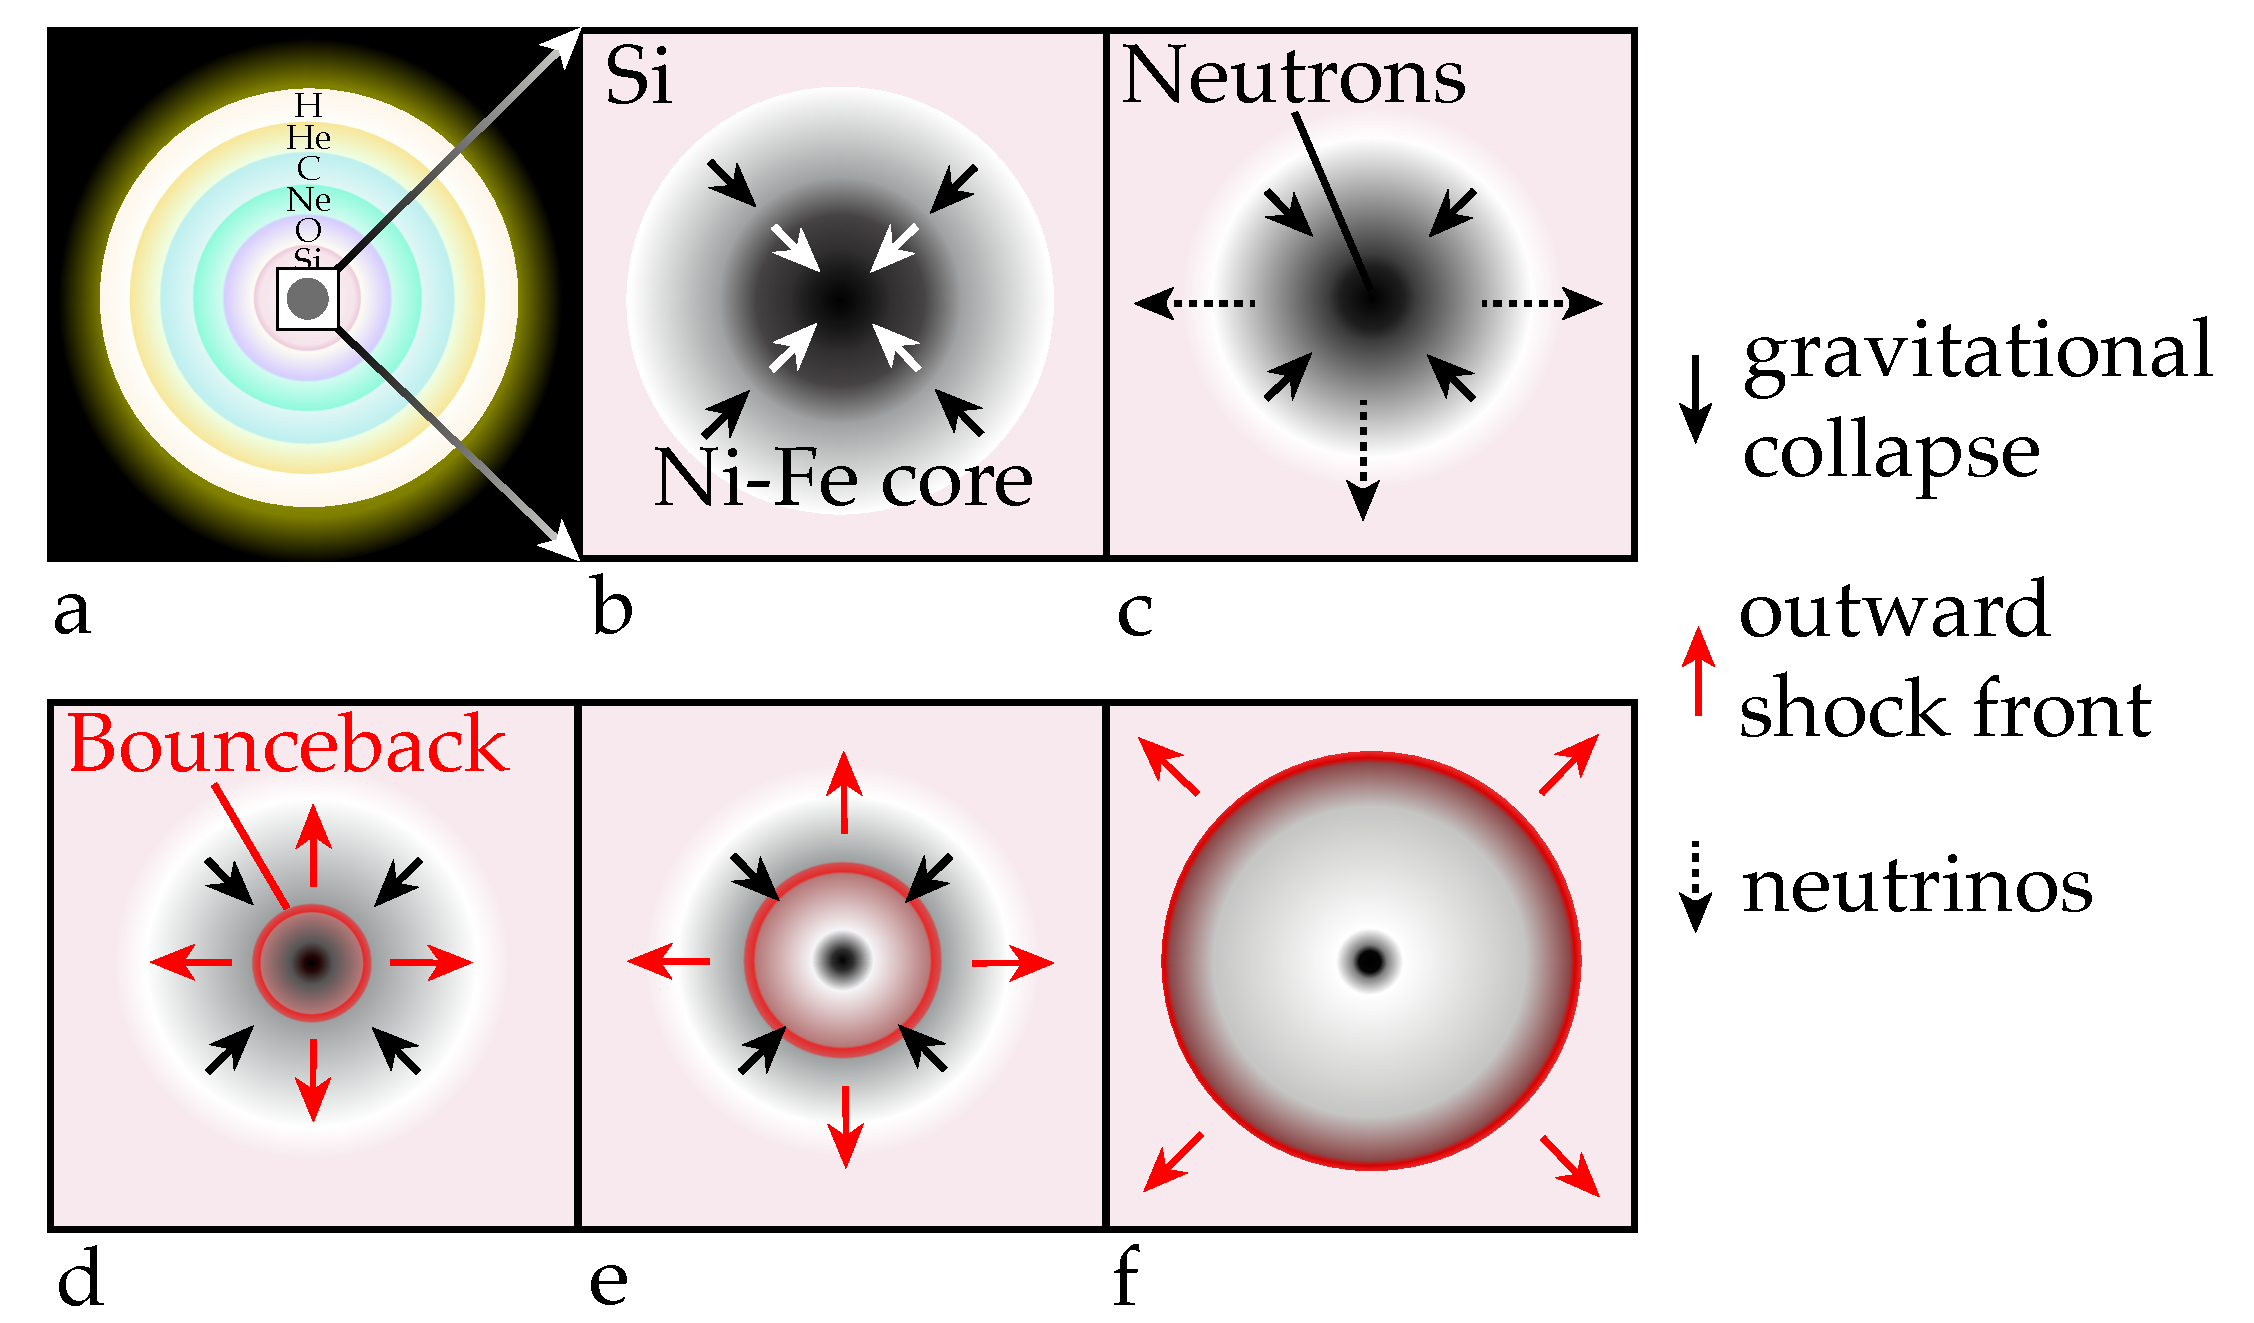
\includegraphics{theory/ccsn.pdf}
    \caption[Core-collapse supernova]{Schematic of a core-collapse supernova. Fusion stops in the core (b), causing it to collapse until neutron degeneracy prevents further collapse. A proto-neutron star forms in the center (c). The infalling material bounces back from the degeneracy border and forms a shock front rapidly moving outwards (d). The stalling shock is reinvigorated by the intense flux of neutrinos from the proto-neutron star (e) and expands further outwards (f). Adapted from \url{https://commons.wikimedia.org/wiki/File:Core_collapse_scenario.png} (which is most likely adapted from~\cite{Janka2012}).}
    \labfig{ccsn_schematic}
\end{figure}

A CCSN happens when a star with a mass between $8$ and $140~M_\odot$ has reached its final fusion stage---silicon burning---which ultimately produces iron. Iron has the highest binding energy of all elements. Therefore, fusing iron to heavier elements would release no energy, and the fusion chain stops. With the fusion in the core subsided, the radiation pressure that so far prevented the star from collapsing in on itself suddenly decreases, and the infalling material compresses the core of the star within a second. As soon as the core becomes incompressible due to neutron degeneracy pressure described by the Pauli exclusion principle, the infalling material bounces back from the incompressible core and blows out into space. The remaining neutron star at the center either survives, or the infalling material eventually causes it to overcome neutrino degeneracy pressure and collapse into a black hole~\cite{Alsabti2017}.~

The more massive the star, the higher the radiation pressure from fusion. This radiation pressure is what drives the shedding of outer layers, so it is assumed that the most-stripped events---SNe Ic---result from a collapse of the most massive stars, followed by SNe Ib and lastly `regular' Type II supernovae, which are powered by stars having largely retained their outer shells.

In the centers of these core-collapse supernovae, neutron stars with masses of $1.5-2~M_\odot$ are created. These need to release large amounts of gravitational binding energy during the short moment of their creation. Because the environment at the center of the CCSN is dense and optically thick, photons are unable to escape: They immediately produce electron-positron pairs, which are in turn quickly absorbed by the surrounding matter.

Instead, \SI{99}{\percent} of the binding energy is carried away by low-energy neutrinos (see panels (e) and (f) in Fig.~\ref{fig:ccsn_schematic}). The energy radiated by the nascent neutron star via neutrinos typically amounts to \SI{\sim1.5e53}{\erg}, distributed equally over all three neutrino families, with a typical energy carried per neutrino of $\mathcal{O}(\SI{10}{\mega\eV})$~\sidecite{Lunardini2017}.

The exact role neutrinos play in core collapses is still insufficiently understood, as one has to rely on data from \emph{SN1987a} only, supplemented by numerical simulations. Eventually, a CCSN within our galaxy might come to the rescue~\sidecite{Janka2017}.

\section{Cosmic Rays}\label{cosmic_rays}

Now, there might also be more energetic neutrinos from space. But as these are thought to be produced during the same processes as cosmic rays, high-energy neutrinos and cosmic rays are intricately linked. Therefore, one first needs a basic understanding of cosmic rays to understand high-energy neutrino production.

\begin{marginfigure}
    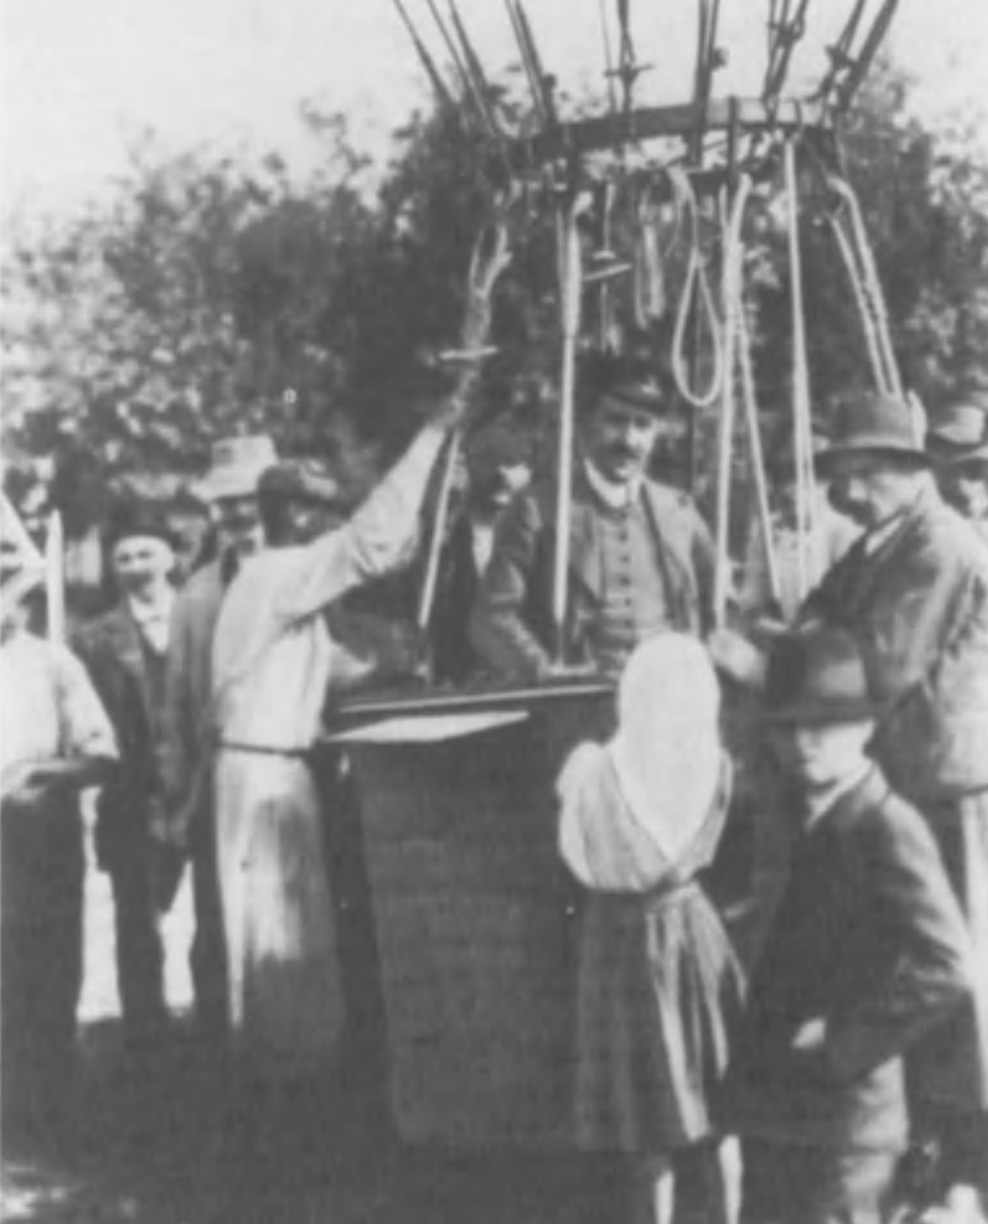
\includegraphics{theory/hess_balloon.png}
    \caption[Hess in his balloon]{Hess in his balloon after landing in Brandenburg, Germany in 1912, having just discovered cosmic rays. From~\cite{Steinmaurer1985}.}
    \labfig{hess_balloon}
\end{marginfigure}

\subsection{Discovery}

Cosmic rays were discovered in 1912 by Victor Hess. At the time, it had already been discovered that electroscopes---devices measuring electric charge and voltage---sometimes spontaneously discharged. This was attributed to particles ionizing the air in the vessel, making it conductive and therefore allowing it to discharge. This was corroborated by the fact that reduced air pressure would slow the speed of the discharge. Another hint was that when shielding the isolated vessel, the ionization would decrease. The source of these ionizing particles was unknown, though.

Hess measured the flux of ionizing radiation with three electrometers during several hot-air balloon journeys. In total, he carried out ten ascents in the years from 1911 to 1913. The first ascent over \SI{5}{\km} in August 1912 marked the discovery of cosmic rays, when he registered a 16-fold increase in ionization measured by the electrometers at that altitude. Hess consequently concluded that the ionizing radiation must be of extra-terrestrial origin~\sidecite{Steinmaurer1985}.

\subsection{Composition and Energy Spectrum}

More than a century later, we know that this ionizing radiation consists of massive particles, spanning a broad range of energies. They are mostly protons, but all stable charged particles and nuclei with lifetimes of $\mathcal{O}(\SI{e6}{\year})$ can be found; most prominently protons, electrons, helium, but also e.g.\ carbon, oxygen and iron~\sidecite{Workman2022}.

As can be seen in Fig.~\ref{fig:cr_spectrum}, the cosmic ray spectrum spans a wide range of energies, from a few \unit{\mega\eV} up to \unit{\zetta\eV}, with the high end of the energy spectrum constituting Ultra High-Energy Cosmic Rays (UHECR).

\begin{marginfigure}
    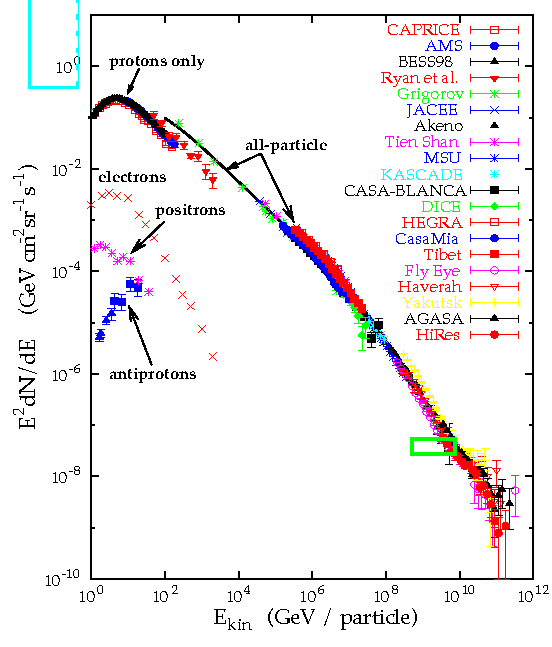
\includegraphics{theory/cr_spectrum.pdf}
    \caption[Cosmic ray spectrum]{Cosmic ray spectrum, as seen by a range of experiments. Adapted from~\cite{Hillas2006}.}
    \labfig{cr_spectrum}
\end{marginfigure}

The UHECR part of the energy spectrum is shown in Fig.~\ref{fig:uhecr_spectrum}. It can be described by a series of power laws with different spectral indices, i.e. $E^{-\gamma}$, with $\gamma$ being the spectral index. The UHECR spectrum shows several interesting features, dubbed the Knee, the anatomically challenging Second Knee, and the Ankle. These are the points where the spectral index changes, and which are possibly associated with a transition to a new source class, e.g.\ from galactic to extragalactic sources around the ankle (see~\sidecite{Taylor2016}). This is still an active field of research~\cite{Workman2022}.

If high-energy neutrinos are produced in the processes responsible for the creation of cosmic rays (see below), the neutrinos stemming from cosmic rays with energies higher than the ankle should be mainly produced by extragalactic sources~\sidecite{Halzen2006}.

\begin{figure}[htb]
    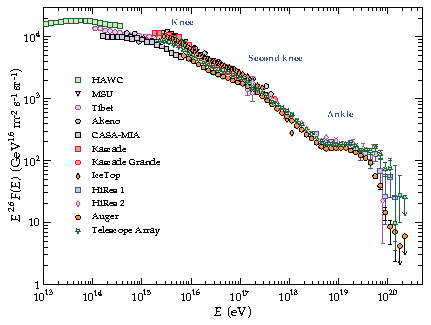
\includegraphics[width=0.8\textwidth]{theory/cr_uhecr_spectrum.pdf}
    \caption[UHECR spectrum]{Ultra high-energy cosmic ray spectrum. It shows energy per particle/nucleus vs.\ the flux (multiplied by $E^{2.6}$ to highlight the changes in spectral index). The data stems from various air-shower experiments. Adapted from~\cite{Workman2022}.}
    \labfig{uhecr_spectrum}
\end{figure}

Identifying the sources of UHECR remains a challenge. As the cosmic-ray particles are charged, they are deflected by magnetic fields encountered on their way to Earth, obscuring their origin. What is known though is that their extremely high energies necessitate extreme production environments.

\begin{marginfigure}
    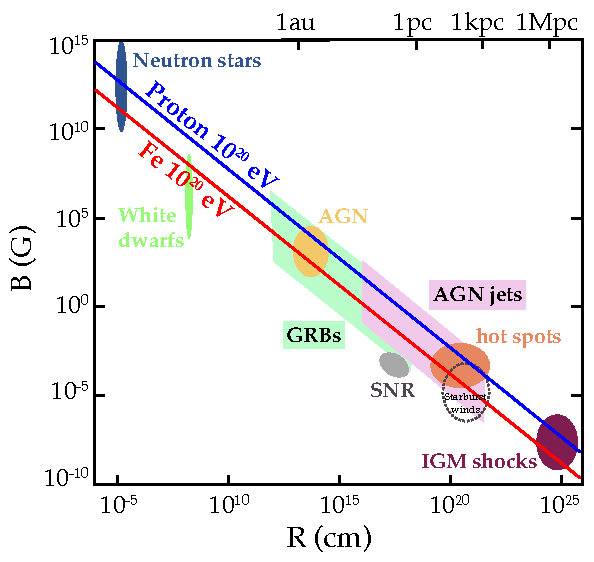
\includegraphics{theory/uhecr_hillas_criterion.pdf}
    \caption[Hillas source distribution]{Possible sources for \SI{e20}{\eV} cosmic rays as a function of source radius $R$ and the magnetic field strength $B$ of the source. Adapted from~\cite{Rieger2022}, the original `Hillas plot' can be found in~\cite{Hillas1984}.}
    \labfig{uhecr_hillas_criterion}
\end{marginfigure}

In the 1980s, Hillas proposed the requirement that the efficient acceleration of a charged particle needs an accelerator that is able to confine the particle during acceleration: This means that the source needs to be larger than the particle's Larmor radius~\sidecite{Rieger2022}, i.e.~the radius of the circle a charged particle travels on given an external magnetic field. This introduces a bound on the possible sources for UHECR cosmic ray sources:

\begin{equation}
    E \leq 10^{20} Z \bigg(\frac{B}{\SI{10}{\micro\gauss}}\bigg) \bigg(\frac{R}{\SI{10}{\kilo\parsec}} \bigg)~\unit{\eV},
\end{equation}

where $Z$ is the cosmic ray particle charge number, $B$ is the magnetic field strength of the source, and $R$ is the characteristic source dimension~\cite{Rieger2022}. Sources that match this criterion for the production of UHECR protons and iron nuclei with an energy of \SI{e20}{\eV} are shown in Fig.~\ref{fig:uhecr_hillas_criterion}. As one can see, a variety of extreme environments are possible sources of UHECR. As some of these also hot candidates for the production of high-energy neutrinos, it is instructive to look at the mechanisms involved.

\subsection{Diffusive Shock Acceleration}\label{dsa}
There are several acceleration mechanisms for UHECR. The most important of these processes, Diffusive Shock Acceleration (DSA), was introduced in the late 1970s. DSA is thought to occur in the presence of shocks that are present e.g.\ in core-collapse supernovae (see Section~\ref{sne}). Such shocks are formed when matter, for example in the form of a plasma, is moving with supersonic speed through a surrounding medium.

\begin{marginfigure}
    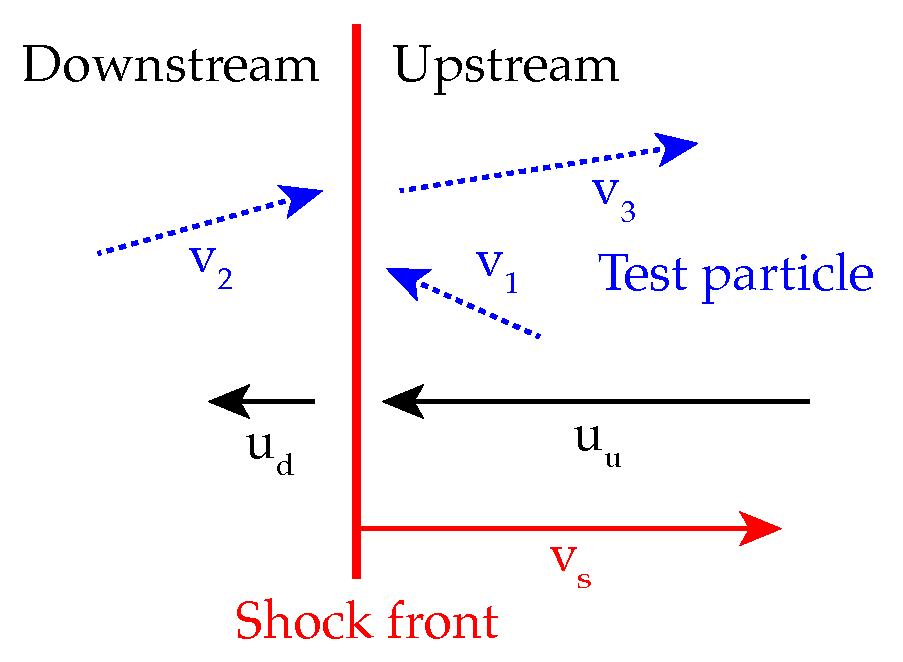
\includegraphics{theory/dsa.pdf}
    \caption[Diffusive shock acceleration]{Sketch illustrating diffusive shock acceleration. A shock front is moving with velocity $v_s$ with respect to an upstream medium. A test particle crosses the shock front twice, each time gaining energy. The length of the arrows are proportional to the velocity.}
    \labfig{dsa}
\end{marginfigure}

To understand DSA, one has to differentiate between an upstream region in front of the moving shock front, and a downstream region behind the shock front.\sidenote{The majority of this section is owed to~\cite{Longair2011}.} Consider a shock front moving with a velocity $\vec{v_s}$ through a medium as seen in the observer's rest frame (red line in Fig.~\ref{fig:dsa}). If we switch to the rest frame of the shock front, it encounters the upstream medium as flowing towards it with speed $\vec{u_u}=-\vec{v_s}$. Downstream, behind the shock, the velocity of material $u_d$ will be lower: Mass conservation requires that $\rho_u u_u = \rho_d u_d$. In astrophysical shocks containing a fully ionized plasma, the compression ratio $R=\rho_d/\rho_u$ can be as high as 4~\sidecite{Longair2011}. Because $R=u_u/u_d$, the velocity of material downstream (behind the shock front) $u_d$ will then only be $1/4 u_u$.

Now consider some test particles upstream, ahead of the shock front rushing towards them. In the rest frame of the upstream gas their velocity distribution will be isotropic. Assume that the diffusion on both sides of the shock front is mediated via collisionless processes. This means that momentum and energy transfers between particles are mediated elastically by magnetic irregularities in the plasma, and Coulomb scattering can be neglected.

When a test particle with initial velocity $v_1$ (blue arrow in Fig.~\ref{fig:dsa}) eventually crosses the shock front to the downstream region, it will see a plasma rushing towards it with speed $w=|u_u-u_d| = (1-0.25)~u_u$, which equals 3/4 of the shock front velocity $v_s$.

\begin{marginfigure}
    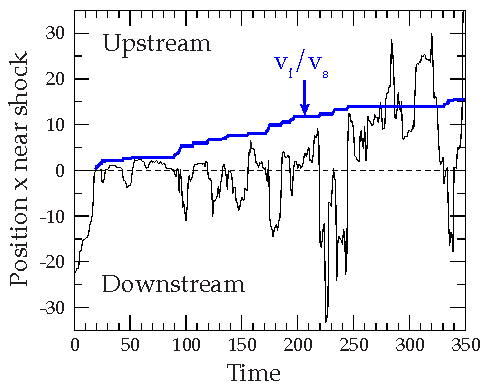
\includegraphics{theory/dsa_mc.pdf}
    \caption[DSA Monte Carlo]{Monte Carlo simulation of a test particle near the shock front. The particle position wildly varies (solid line), but its velocity $v_i$ (blue line) increases each time it crosses the shock front at $x=0$. Adapted from~\cite{Baring1997}}
    \labfig{dsa_mc}
\end{marginfigure}

In the downstream region, they will again be scattered collisionlessly, and receive a small net energy gain of $\big\langle\frac{\Delta E}{E}\big\rangle = \frac{2}{3}\frac{w}{c}$ (see below). This energy gain results in a higher velocity $v_2$. After some time, the particle might cross the shock front again, this time into the upstream region. From the now isotropized particle's frame, the upstream region will again rush in with $0.75~v_s$, and the process repeats, resulting in another gain in energy, and a higher $v_3$~\sidecite{Urosevic2019}, with an average round-trip energy gain of $\big\langle\frac{\Delta E}{E}\big\rangle = \frac{4}{3}\frac{w}{c}$. See Fig.~\ref{fig:dsa_mc} for a Monte Carlo simulation of a test particle crossing a shock front multiple times, accumulating a higher and higher velocity over time (blue line).

We still need to motivate the net energy gain per crossing of $\big\langle\frac{\Delta E}{E}\big\rangle = \frac{2}{3}\frac{w}{c}$. This can be explained as follows: First, one needs to switch to the test particle frame, i.e.\ perform a Lorentz transformation. The energy of the test particle will be:

\begin{equation}
    E' = \gamma_{w}(E+p_x w),
\end{equation}

where x is the coordinate perpendicular to the shock. The shock is non-relativistic ($w<<c$ and $\gamma_w\approx1$), but the test particle is, so $E\approx pc$ and $p_x \approx E/c \cos(\theta)$. From this it follows that

\begin{equation}
    \Delta E = E' - E = E+\frac{E}{c}w\cos{\theta}-E = pw\cos{\theta}
\end{equation}

and

\begin{equation}
    \frac{\Delta E}{E} = \frac{p}{w}\cos{\theta} = \frac{w}{c}\cos{\theta}.
    \label{eqn:delta_e_over_e}
\end{equation}

The probability of the test particle angle $\theta$ to lie between $\theta$ and $\theta + \text{d}\theta$ is proportional to $\sin{\theta}\text{d}\theta$, and the test particle approach rate is proportional to $v_x = \frac{p_x}{m} = \frac{E/c\cos{\theta}}{E/c^2} = c \cos{\theta}$. The probability of the test particle crossing the shock front is therefore proportional to $\sin{\theta} \cos{\theta} \text{d}\theta$. The integral from 0 to $\frac{\pi}{2}$ is 0.5, so we need to multiply by 2 to normalize the cumulative probability to 1:

\begin{equation}
    p(\theta) = 2\sin{\theta}\cos{\theta} \text{d}\theta
\end{equation}

By integrating $p(\theta)$ and using Eq.~\ref{eqn:delta_e_over_e}, we can calculate the average energy gain of each shock crossing:

\begin{equation}
    \bigg\langle \frac{\Delta E}{E} \bigg\rangle = \int_0^{\pi/2} \frac{\Delta E}{E} p(\theta) = \frac{w}{c} \int_0^{\pi/2} 2 \sin{\theta} \cos^2{\theta}  \text{d}\theta = \frac{2}{3}\frac{w}{c}
\end{equation}

After another crossing, the test particle will gain another average energy increase of $\frac{2}{3}\frac{w}{c}$, resulting in an average energy gain of $\frac{4}{3}\frac{w}{c}$ per round trip~\cite{Longair2011}.

During each crossing, a particle with initial energy $E_0$ will gain an energy fraction $\beta$, resulting in energy $E=\beta E_0$. If $P$ denotes the probability that a particle stays within the accelerating region, the number of particles after $k$ crossings can be written as $N=N_0 P^k $, and they will have energies $E=E_0\beta^k$.

If one solves both equations for $k$ and sets them equal, one obtains
\begin{equation}
    \frac{\ln (N/N_0)}{\ln (E/E_0)} = \frac{\ln P}{\ln \beta}.
\end{equation}

By rearranging we get

\begin{equation}
    \frac{N}{N_0} = \bigg(\frac{E}{E_0}\bigg)^{\ln P / \ln \beta}
\end{equation}

To obtain the differential energy spectrum, we differentiate with respect to $E$ and get

\begin{equation}
    \label{eqn:diff_e_spec}
    N(E)~\text{d} E = C\times E^{(\ln P/\ln\beta)-1}~\text{d} E
\end{equation}

The result is a power law with index $\frac{\ln P}{\ln \beta}$, which is indeed what was already stipulated by experimental data.

We already know that $\big\langle\frac{\Delta E}{E}\big\rangle = \frac{4}{3}\frac{w}{c}$ per round trip. With this, $\beta = \frac{E}{E_0} = 1 + \frac{4}{3}\frac{w}{c}$. What is missing is an expression for $P$. To obtain this, we need to estimate the rate at which particles drop out of the system or are `swept away'. As argued by~\cite{Longair2011} (and originally presented by~\sidecite{Bell1978}), the average number of particles crossing the shock is $\frac{1}{4} n c$, with $n$ being the particle number density. This is true in both directions up- and downstream. The difference though is that downstream particles are `advected' away from the shock further downstream and out of the system, as they are isotropic in that frame. The dropout rate is $n w=\frac{1}{4}nv_s$. From this it follows that the fraction of particles lost (per unit time) is $\frac{1}{4} n v_s/\frac{1}{4}nc = v_s/c$. The survival probability $P$ is thus $P=(1-v_s/c)$.

With that, we can compute
\begin{equation}
    \ln P = \ln \big( 1-\frac{v_s}{c}\big) \simeq -\frac{v_s}{c}
\end{equation}
and
\begin{equation}
    \ln \beta = \ln \bigl( 1+\frac{4}{3}\frac{w}{c} \bigr)  \simeq \frac{4}{3}\frac{w}{c} = \frac{v_s}{c}.
\end{equation}
This gives us $\frac{\ln P}{\ln \beta} \simeq -1$. Inserting this into Eq.~\ref{eqn:diff_e_spec} yields
\begin{equation}
    N(E)~\text{d} E \propto E^{-2}~\text{d} E.
\end{equation}

Therefore, the resulting differential energy spectrum has a spectral index of 2, a value that somewhat differs from the experimentally found spectral index of 2.7 up to the knee. This can be explained by the fact there are several assumptions at play here: The shock is assumed to be non-relativistic, situated in an ideal gas and with a constant escape probability. Inefficiencies in the shock, and the inclusion of shock-amplified magnetic fields can both harden the spectral index~\cite{Spurio2018}.

\subsection{Interaction and Neutrino Production}\label{cr_interactions}
As discussed above, the observed cosmic ray spectrum is readily explained by astrophysical shocks, as these account for the power-law structure of the energy distribution.

The particles accelerated within shocks might now interact with either hadrons and photons in their vicinity or on their way to Earth. For simplicity, this section focuses on the interaction of cosmic-ray protons, but it applies to heavier nuclei as well.

\begin{description}
    \item[$pp-$interactions] When cosmic-ray protons encounter gas, either at the source location or while crossing the universe, they can interact with this gas, here assumed to consist of protons only for simplicity. The resulting $pp$-interactions produce lots of unstable hadrons, which decay. Those decays are dominated by pion production. Ignoring all secondary hadrons $X$ (which can also decay via pions), possible decay channels of these pions are:

          \begin{eqnarray}
              \pi^\pm + X &\contour{black}{$\rightarrow$}& \mu^\pm + \nu_\mu (\bar{\nu}_\mu)~~~ \contour{black}{$\rightarrow$} ~~~ e^\pm + \nu_e(\bar{\nu}_e) + \bar{\nu}_\mu(\nu_\mu)\text{,}\\
              \pi^0 + X &\contour{black}{$\rightarrow$}& 2\gamma.
          \end{eqnarray}
          As can be seen, $\pi^\pm$ decay into muons and a muon (anti-) neutrino. Those muons will decay into electrons (positrons), electron \mbox{(anti-)}~neutrinos and muon (anti-) neutrinos. The decay of the neutral $\pi^0$ does not generate neutrinos. For pion decays, an average neutrino flavor content of $\nu_e$:$\nu_\mu$:$\nu_\tau = 1:2:0$ is expected. Neutrino oscillations on the way to Earth wash out this initial difference, with an expected final flavor content of $1:1:1$~\cite{Workman2022}.
          \\
          \\
          The energy of the pion decay products is expected to trace the initial proton energy spectrum. If the proton interaction rate is fairly independent of their energy, they will then lose a fraction of their energy. This energy will then be converted into the production of pions, and subsequently muons. With this, the resulting neutrino spectrum is expected to have a similar shape as the initial cosmic ray spectrum~\sidecite{Fiorillo2023}.
          \\
          \\


    \item[$p\gamma-$interactions]
          Cosmic-ray protons can also interact with radiation fields. The cross-section for these interactions is large near the $\Delta^+$ resonance. The dominant $\Delta^+$ decay modes also contain pions:
          \begin{eqnarray}
              \Delta^+ ~~ &\contour{black}{$\rightarrow$}& n + \pi^+ \\
              \Delta^+ ~~ &\contour{black}{$\rightarrow$}& p + \pi^0
          \end{eqnarray}
          The pions will again decay according to the channels already discussed for $pp$-interactions. The secondary neutrons might decay via beta decay, and produce electron antineutrinos. Here, the shape of the neutrino spectrum not only depends on the proton spectrum, but also the photon spectrum. Therefore, it is not expected to trace the shape of the initial cosmic-ray spectrum~\sidecite{Fiorillo2021}.
\end{description}


\section{High-Energy Neutrino Astronomy}\label{he_neutrino_astronomy}

As shown above, high-energy cosmic ray particles can produce high-energy neutrinos in $pp$- or $p\gamma$-interactions. These high-energy neutrinos have energies in the \unit{\mega\eV} range and above. But what are possible source classes for these? There will be some overlap with the low-energy neutrino events, as some of those---like e.g. supernovae---are also probable sources of high-energy neutrinos.

\subsection{Interacting Supernovae}\label{interacting_sne}
As already detailed in Section~\ref{sne}, core-collapse supernovae are thought to produce copious amounts of \unit{\mega\eV}-neutrinos. Interestingly, certain types of CCSNe are thought not only to produce such comparably low-energy neutrinos, but also \unit{\giga\eV} to \unit{\tera\eV} neutrinos. Optical observations have stipulated that supernova progenitors often violently eject material into the circumstellar region in the years or centuries prior to their explosion~\sidecite{Ofek2014}. When the supernova happens, ejecta are driven into this circumstellar material (CSM).

SNe of Type IIn are a subclass first stipulated by Schlegel~\sidecite{Schlegel1990}: The Balmer emission features of early IIn spectra, most prominently the $H_\alpha$ region, show narrow lines on top of a broad component~\sidecite{Taddia2013}. The broad component is caused by the supernova itself, but the narrow lines result from interaction of the SN blast-wave with the CSM. This process photo-ionizes the CSM, which results in narrow hydrogen lines.

Such a system might be promising for the production of high-energy neutrinos, as highlighted in~\sidecite{Kurahashi2022}. When the SN ejecta, expanding with velocities of \SIrange{3000}{10000}{\km\per\s}, hit the CSM, a shock wave starts to propagate through the CSM. Particle acceleration within the shock is predicted to happen at the moment of shock breakout. This is the time when the optical depth of the shock drops below $\approx c/v$, with $v$ being the shock velocity. As soon as the radiation can escape, the shock is no longer radiation-mediated, and protons can be accelerated to high energies via diffusive shock acceleration (see Section~\ref{dsa})~\sidecite{Waxman2017}. This emission seizes after the shock decelerates or reaches the outer edge of the CSM.

These accelerated protons are expected to generate high-energy neutrinos, either by $pp$- or $p\gamma$-interactions (see Section~\ref{cr_interactions}). The resulting neutrinos' energies might range from \unit{\giga\eV} to hundreds of \unit{\tera\eV}, reaching their maximum flux shortly after shock breakout~\sidecite{Petropoulou2017,Murase2018}.

The signature of such an event is a high-energy neutrino detected close to the optical peak of a supernova that shows signs of CSM interaction, i.e.\ the hydrogen lines in the spectrum have a narrow component.

\subsection{Gamma-ray Bursts}\label{grb}
Gamma-ray bursts (GRBs) were discovered by accident by the \textit{Vela} satellites designed to monitor nuclear detonations as part of a partial test ban treaty between the US and the USSR in the 1960s. 16 bursts of high-energy photon events recorded by those satellites were published in 1973. This kicked off a flurry of research, as a terrestrial or solar origin of these gamma-ray bursts could be excluded based on light travel time differences allowing a rough triangulation of the signals~\sidecite{Klebesadel1973}.

The gamma-ray light curves of these very bright and brief events last from a few milliseconds to tens, sometimes hundreds of seconds~\sidecite{Vedrenne2009}. As more and more GRBs were registered, a bimodal population was recognized: Short GRBs (sGRBs), with an average duration of \SI{\sim0.3}{\s}, and long GRBs (lGRBs) that typically last \SIrange{10}{20}{\s}.

\begin{description}
    \item[Short GRBs] The most prevalent interpretation of these two populations is that short GRBs stem from the merger of two compact objects, e.g.~neutron stars. This was hypothesized for a long time, and found spectacular confirmation with the association of the short gamma-ray burst \textit{GRB170817A} detected \SI{1.7}{\s} after a gravitational wave signal was registered from the same region (\textit{GW170817}), most likely stemming from the merger of two neutron stars~\sidecite[-20pt]{Abbott2017}.

    \item[Long GRBs] Meanwhile, long GRBs are hypothesized to be the signatures of jets launched by CCSNe~\sidecite{Galama1998}. The existence of such jets has been proposed already in the 1970s; see e.g.~\sidecite{Leblanc1970}. If these jets manage to punch through the stellar envelope and the surrounding CSM, one can detect them as long GRBs. Virtually all CCSNe that have been associated with a prior long GRB were Broad-Line Ic (Ic-BL)~\sidecite{Pian2017}, i.e.\ collapses of highly stripped, massive stars with large ejecta velocities.
\end{description}

Both short and long GRBs have been proposed as potential sources of high-energy neutrinos. For short GRBs, neutrinos are only attributable to a source if a GRB afterglow is detected, i.e.\ longer-lasting X-ray, optical and radio emission~\sidecite{Waxman1997}. The event signature as accessible by IceCube and ZTF (see next two chapters) would be a prompt high-energy neutrino coincident with the gamma-ray signal, accompanied by optical emission quickly fading over the subsequent days.

\begin{figure*}[htb]
    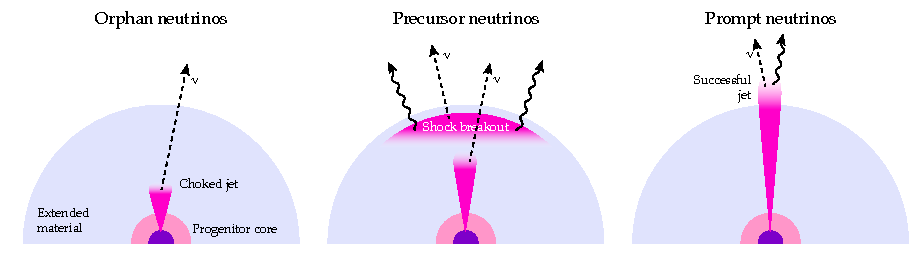
\includegraphics[width=1.5\textwidth]{theory/grb_model.pdf}
    \caption[High-energy neutrinos from GRBs]{Concordance scenario for neutrinos from failed, semi-failed and successful jets launched by CCSNe.\ Left: The jet fails to punch through the environment, resulting in orphan neutrinos from the jet without any photons, as no GRB is produced.\ Middle: Here, the jet fails too, but triggers a shock breakout, resulting in a second wave of neutrinos, accompanied by a low-luminosity gamma-ray signal (low-luminosity GRB).\ Right: The jet launches successfully, generating prompt neutrinos accompanied by gamma-rays (long GRB). Adapted from~\cite{Senno2016}.}
    \labfig{grb_model}
\end{figure*}

Long GRBs on the other hand are also predicted to produce high-energy neutrinos~\sidecite{Meszaros2001}. One needs to distinguish three different scenarios, as illustrated in Fig.~\ref{fig:grb_model}:
\begin{description}
    \item[Choked jet (left panel)] If the jet launched by the stellar collapse fails to penetrate the stellar and CSM environment and chokes, no light would is visible, only orphan high-energy neutrinos from the choked jet emerge, without an electromagnetic counterpart.
    \item[Choked jet with shock breakout (middle)] If the choked jet manages to trigger a shock breakout (see Section~\ref{interacting_sne}), both the neutrinos from the choked jet (precursor neutrinos) and delayed high-energy neutrinos accompanied by a low-luminosity GRB and afterglow emission from the shock breakout are visible.
    \item[Successful jet (right)] If the jet successfully launches, a long GRB accompanied by high-energy neutrinos is expected within minutes after the stellar collapse.
\end{description}

In all cases, further evolution will lead to an emerging supernova---most likely of Type Ic-BL---which will be detectable at the location of the neutrino in optical bands in the following weeks~\sidecite[-20pt]{Senno2016}.

\subsection{Active Galactic Nuclei}\label{agn}
Another extreme environment are active galactic nuclei (AGN). At the center of most galaxies lies a supermassive black hole (SMBH). If the region around the SMBH is active, the system is considered an AGN. The key features of AGN explain what `active' means: AGN are highly luminous, with bolometric luminosities up to \SI{e48}{\erg\per\s}. They vary on rapid timescales, which allows to infer that the emitting regions must be small (to not violate causality). Also, their luminosity function (the number of AGN per luminosity bin) evolves strongly with redshift. Lastly, AGN emit throughout the electromagnetic spectrum~\sidecite{Padovani2017a}.

The history of AGN research began in the 1940s, when Grote Reber detected strong radio sources on the sky, among them Cygnus A, now known to be an AGN. Around the same time, Carl Seyfert discovered a type of galaxy with luminous nuclei~\sidecite{Seyfert1943}. In 1963 Maarten Schmidt discovered a point-like object (3C 273) with a redshift of 0.158, using the P200 on Mount Palomar (see Chapter~\ref{ztf}). The large redshift ruled out that the source was a regular star. Rather, it was located in the nucleus of a galaxy with the same redshift. The remarkably large luminosity he inferred from that was about 100 times brighter than comparable galaxies~\sidecite{Schmidt1963}.

Today we assume that most galaxies contain a SMBH at their center. If the accretion rate, i.e.\ the rate at which the SMBH accumulates mass, is high, the galaxy appears active. We also assume that the myriad of different types of active galaxies (blazars, Seyfert I and II galaxies, radio-loud galaxies, etc.) are all appearances of intrinsically similar objects: They are merely a function of the viewing angle at which we look at the AGN system, plus the presence or absence of a jet launched by the system (and the accretion rate of the SMBH).

\begin{figure}[htb]
    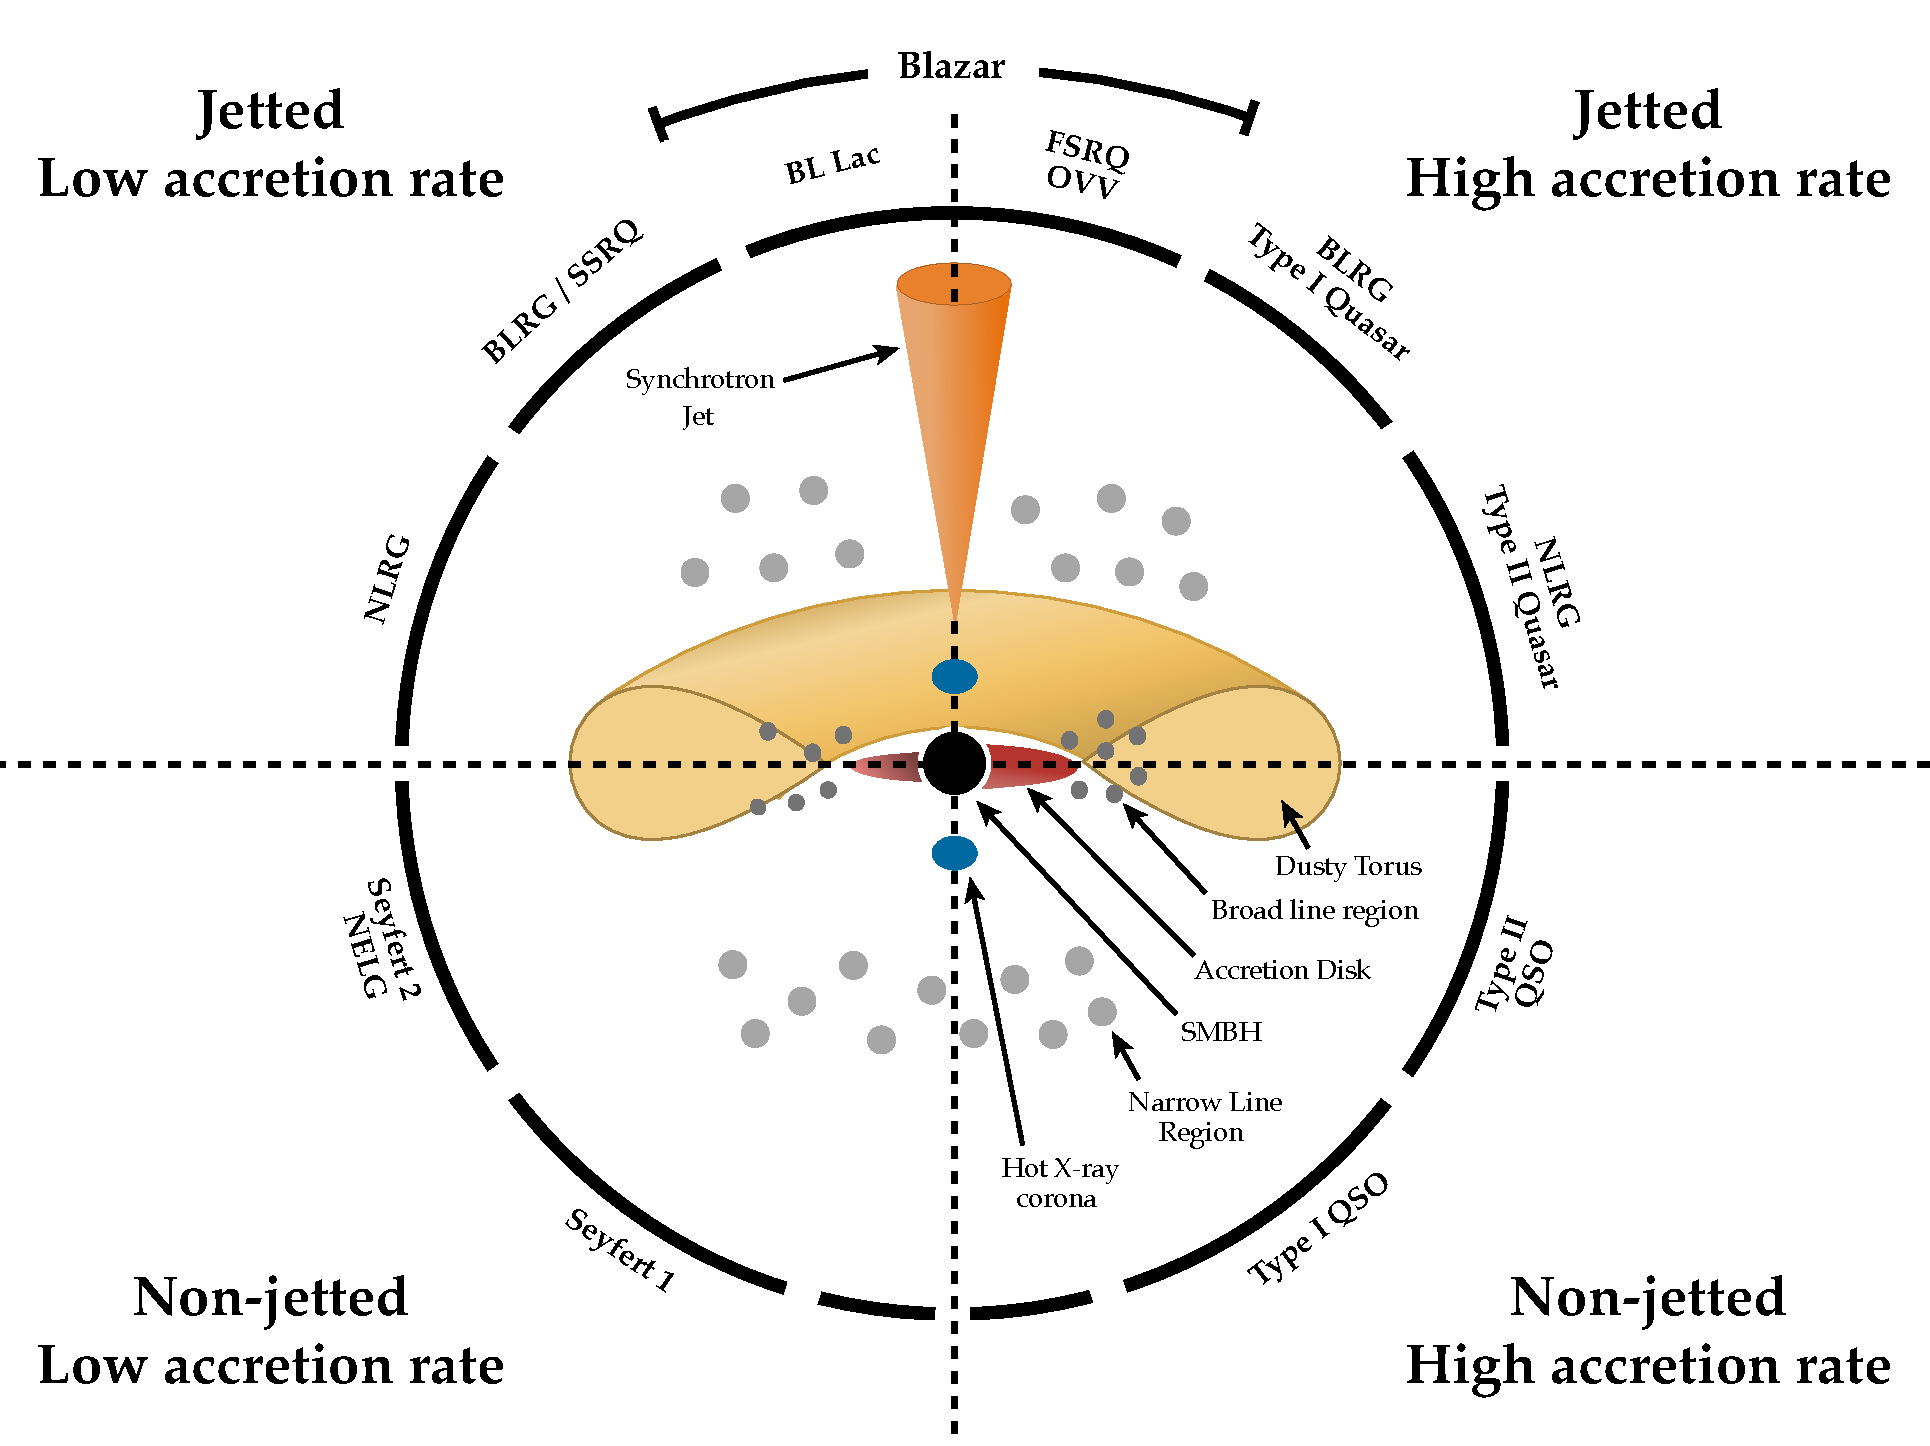
\includegraphics[width=0.9\textwidth]{theory/agn_unification.pdf}
    \caption[AGN unification scheme]{AGN unification scheme. Depending on the viewing angle towards the AGN system, different source classes emerge. Following the argumentation of~\cite{Padovani2017}, the upper (lower) segment label radio loud (radio quiet) was changed to jetted (non-jetted). Adapted from~\cite{Thorne2022}.}
    \labfig{agn_unification}
\end{figure}

As can be seen in Fig.~\ref{fig:agn_unification}, these systems are thought to contain a SMBH at the center. The black hole is fed by a surrounding accretion disk of hot material, which in turn is enshrouded in a dusty torus.

Often, energetic jets of relativistic material are launched from the system, perpendicular to the accretion disk. When one looks directly into the jet, the system appears as blazar (top of~\ref{fig:agn_unification}). If one moves away from the jet direction, the AGN will in general appear as Type I AGN, displaying broad emission lines stemming from the so-called Broad-Line Region (BLR), lying at a distance of \SIrange{0.01}{1}{\parsec} to the SMBH. The BLR consists of gas clouds, and the Doppler-induced line-broadening suggests high velocities, resulting from the fact that the material is deep within the gravitational well of the SMBH.

\begin{marginfigure}
    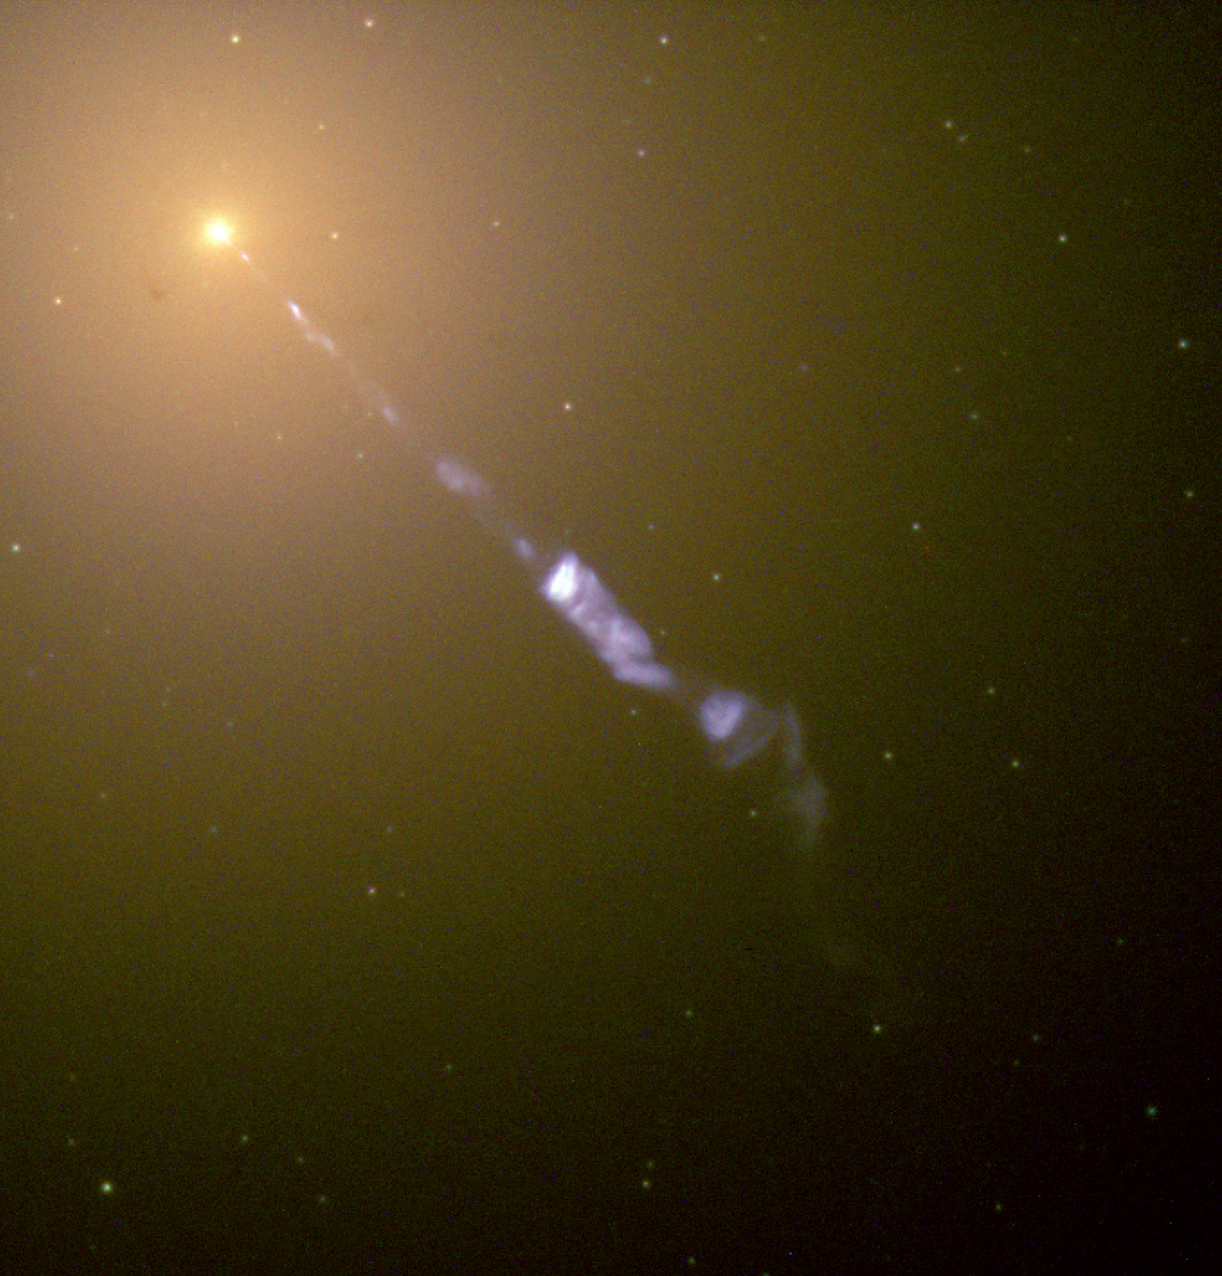
\includegraphics{theory/m87.jpg}
    \caption[\textit{M87} jet]{Hubble Space Telescope composite image of the jet launched by the AGN in \textit{M87}, \SI{17}{\mega\parsec} away. The large size of the SMBH in \textit{M87} made it the first target of the Event Horizon Telescope, resulting in the first direct image of a black hole ever taken~\cite{Akiyama2019}. Image credit: NASA/Hubble Heritage Team.}
    \labfig{m87_jet}
\end{marginfigure}

Moving yet further away from the jet, one gradually enters the regime of the Type II AGN: The BLR close to the core gets hidden behind the dust torus, and only the  Narrow-Line Region (NLR) is still visible, as it is more distant from the core (\SIrange{e2}{e4}{\parsec}). Here too, gas heated by the core radiates, but the gas density is lower compared to the BLR, and from the line-broadening one can infer much lower velocities of \SI{\sim500}{\kilo\m\per\s}~\sidecite{Beckmann2012}.

If a jet is present, the AGN strongly emits in radio wavelengths. This is caused by the synchrotron emission of highly relativistic electrons. These AGN were labeled `radio loud', in contrast to `radio quiet' AGN without a jet.

AGN have been proposed as sources of high-energy neutrinos as early as the 1970s~\sidecite{Eichler1979}. The most promising site of high-energy neutrino production is the relativistic jet. In some cases such jets can be visually detected, like the prominent jet visible in \textit{M87} (see Fig~\ref{fig:m87_jet}). Jets are thought to be highly collimated, extremely energetic plasma structures launched from the accretion disk. Only a minority of \SIrange{10}{20}{\percent} of observed AGN show evidence of such jets~\sidecite{Padovani2010}. The intrinsic fraction of jetted AGN is considerably lower, with an estimate of \SIrange{0.1}{0.2}{\percent}.

When the electrons and protons contained in the jet plasma are clumped together in relativistically moving `blobs' and are spinning in magnetic fields, they emit synchrotron radiation. This is the usual explanation for the first hump in a typical blazar spectral energy distribution (SED)~\sidecite{Combes2021}.

\begin{marginfigure}
    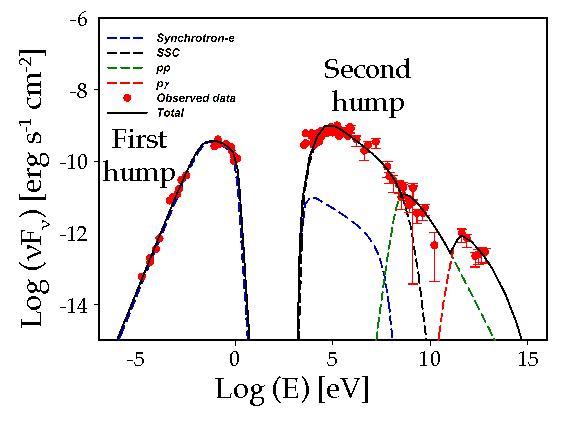
\includegraphics{theory/agn_two_humps.pdf}
    \caption[Typical AGN spectrum]{Typical AGN spectrum, showing two humps. Adapted from~\cite{Khiali2015}.}
    \labfig{agn_typical_sed}
\end{marginfigure}

The explanation for the second hump is still debated. One scenario is that the synchrotron photons themselves form a target field for their `parent' electrons and protons. The electrons and protons can interact with these photons via inverse Compton Scattering (CS), transferring energy to the photons. This process is called Synchrotron Self-Compton (SSC)~\cite{Spurio2018}, giving rise to the second hump. This was dubbed the Leptonic Model, and due to the absence of accelerated hadrons like protons, it does not predict the presence of high-energy neutrinos.

An alternative model to explain the second hump is the Hadronic Model. Here, in addition to leptons, the jet also contains a sizable fraction of hadrons~\sidecite{Reimer2012}. So not only the leptonic processes take place (synchrotron radiation, inverse Compton scattering), but also the protons generate synchrotron radiation. Additionally, the hadrons can interact with target photons in the vicinity, producing charged and neutral pions. These decay as detailed in Section~\ref{cr_interactions}, producing high-energy neutrinos in the process. Therefore, the detection of high-energy neutrinos from blazars is considered a smoking gun signature for hadronic acceleration processes~\sidecite{Gao2018}.

As the AGN's optical brightness is driven by the synchrotron emission, it only traces the photon target field density for potential hadronic interactions, but not the proton luminosity itself.

\subsection{Tidal Disruption Events}
The last class of potential high-energy neutrino sources discussed here are Tidal Disruption Events (TDEs). A TDE marks the end of a very unlucky star. When a star happens to approach the SMBH at the galactic center too closely, the resulting gravitational forces might overcome the star's self-gravity, tidally disrupting and destroying the star in the process~\sidecite{Rees1988}. Roughly half the mass of the star is accreted around the black hole, and the bright electromagnetic flare created by this can shine for months. Nevertheless, the exact mechanisms at play causing this emission are still widely discussed~\sidecite{Gezari2021}.

\begin{marginfigure}
    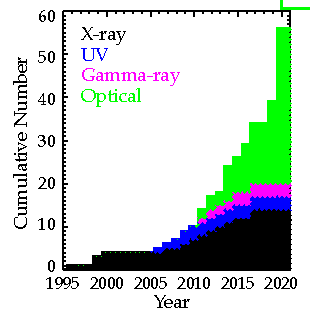
\includegraphics{theory/tde_cumulative.pdf}
    \caption[TDE detections]{Cumulative number of TDE detections, with the color encoding the discovery wavelength. The relative increase in the detection rate is driven by ZTF\@. Adopted from~\cite{Gezari2021}.}
    \labfig{tde_cumulative}
\end{marginfigure}

TDEs have already been predicted in the 1970s~\sidecite{Hills1975}, and the first few of them were discovered in the 1990s and early 2000s in X-ray wavelengths. Optically detected TDEs arrived in the last decade~\sidecite{Velzen2011}, with steadily rising numbers in the last years, mainly driven by optical all-sky survey telescopes like the Zwicky Transient Facility (ZTF, see Chapter~\ref{ztf}). Fig.~\ref{fig:tde_cumulative} shows the number of detected TDEs since 1995. As of 2022, roughly 100 TDEs have been discovered in total, with more than 30 detected during the 2.6 years of ZTF Phase I alone~\sidecite{Hammerstein2022}.

TDEs normally emit a continuous spectrum that can be well-approximated by a blackbody (see e.g.~\sidecite{Gezari2015} for a spectrum of \textit{PS1-10jh}, the prototypical optical/UV TDE). Peculiarly, there seems to be a somewhat bimodal distribution of blackbody temperatures: One optical/UV population, and a second population peaking in the X-ray, better described by blackbodies of higher temperature~\cite{Gezari2021}.

As the accretion disk hypothesized  to form from the infalling material after the disruption will most likely be very hot, it is unclear what the cause of the optical/UV emission is. Furthermore, the blackbody radii inferred from the optical/UV emission exceed the size of the freshly formed accretion disk by $1-2$ orders of magnitude.

To date, multiple models have been brought forward to motivate the optical/UV emission, such as semi-relativistic outflows or winds, or diffusive shock acceleration stemming from the tidal stream intersecting itself~\cite{Gezari2021}.

\begin{figure}[htbp]
    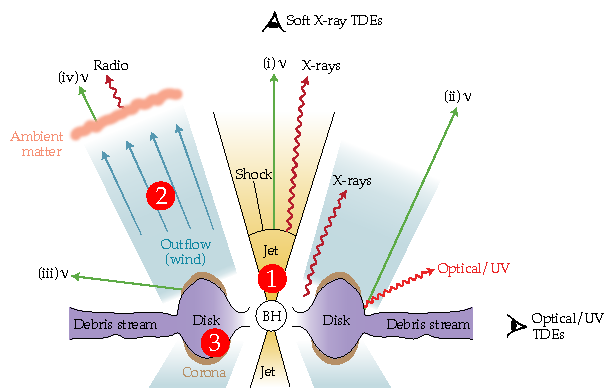
\includegraphics[width=0.9\textwidth]{theory/tde_unification.pdf}
    \caption[TDE Unification]{TDE unification model. The peak wavelength visible is a function of the viewing angle. Seen from above, the X-rays are dominating, while viewed edge-on, the TDE appears in the optical/UV\@. Possible sites of high-energy neutrino production are shown as numbered red circles. Adopted from~\cite{Hayasaki2021}.}
    \labfig{tde_unification}
\end{figure}

If the material from the disrupted star is circularized rapidly, one interesting approach to unify the two populations is a viewing angle dependent model, akin to the unified AGN model presented in Section~\ref{agn}.

In this model, which is shown in Fig.~\ref{fig:tde_unification}, TDEs appear X-ray bright when one looks into the direction of a shocked jet perpendicular to the accretion disk. Optical/UV TDEs are systems viewed more edge-on, where X-rays are obscured, and emission stems mainly from X-rays reprocessed in the outer disk or in outflows~\sidecite{Hayasaki2021}. Intermediate viewing angles will produce a mixture of both signals.

About \SI{1}{\percent} of TDEs are expected to launch relativistic jets, like e.g.\ the recently discovered \textit{AT2022cmc}~\sidecite{Andreoni2022}. Such jets, denoted as (1) in Fig.~\ref{fig:tde_unification}, as well as the possible winds/outflows (2) or a potentially present disk corona (3), have all been proposed as production sites of high-energy neutrinos, shown as green lines (see e.g.~\sidecite{Murase2020} for the non-jet production sites, and~\sidecite{Liu2020} for a jet scenario).

The timescales involved in the neutrino production are poorly constrained, as the systems are not very well understood yet. It is to be expected though that neutrino production would not predate the TDE and optical emission from the event.

\section{Established Counterparts and Limits}

\begin{figure}[htb]
    \centering
    \begin{subfigure}[b]{0.52\textwidth}
        \centering
        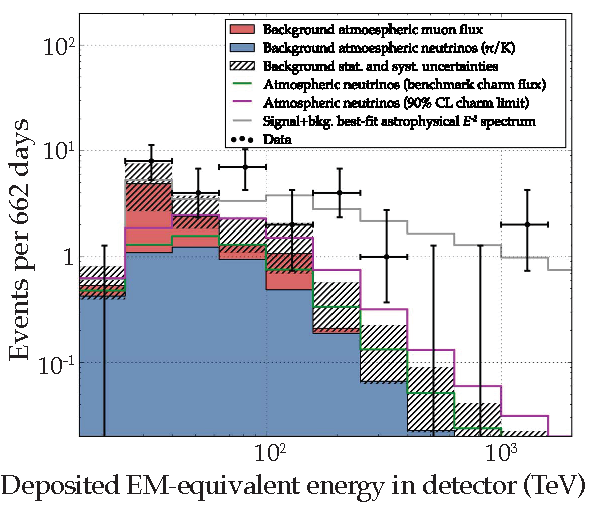
\includegraphics[width=1\textwidth]{theory/ic_first_spectrum.pdf}
    \end{subfigure}
    \begin{subfigure}[b]{0.47\textwidth}
        \centering
        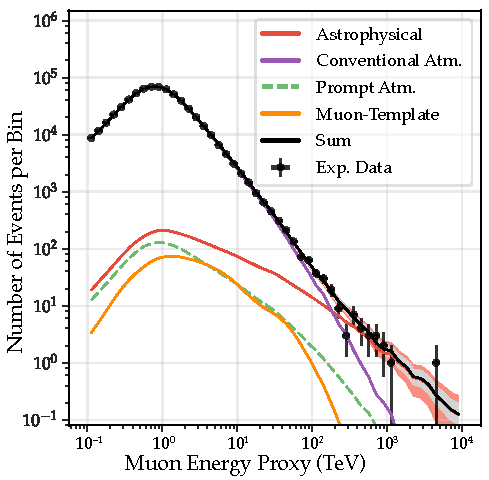
\includegraphics[width=1\textwidth]{theory/ic_last_spectrum.pdf}
    \end{subfigure}
    \caption[Astrophysical neutrino spectrum]{Left: Energy spectrum of the first astrophysical neutrinos, as detected by IceCube in 2013. The black points are the neutrinos measured, binned in energy deposited in the detector (a lower bound on the neutrino energy). The expected background rate of atmospheric muons (neutrinos) is shown in red (blue), and the gray line shows the best-fit astrophysical spectrum ($E^{-2}$ plus background).\ Right: Latest measurement of astrophysical neutrinos from a selection of track-like events (see Section~\ref{reconstruction}), including 9 years of IceCube data. Also here, the binned measurements are shown in black. Adapted from~\cite{Aartsen2013,Abbasi2022b}.}
    \labfig{ic_first_spectrum}
\end{figure}

In 2013, IceCube, a cubic-kilometer scale Cherenkov detector located within the Antarctic ice at the South Pole (see next Chapter~\ref{ic} for details) first detected two likely astrophysical \unit{\peta\eV} neutrinos at a significance of \SI{2.8}{\sigma}~\sidecite{Aartsen2013b}. Later that year, IceCube published more data, detecting high-energy astrophysical neutrinos at a confidence level of \SI{4}{\sigma}~\sidecite{Aartsen2013}.

Fig.~\ref{fig:ic_first_spectrum} shows the first energy spectrum of high-energy neutrinos published by IceCube (left), as well as a more recent measurement from 9 years of IceCube data (right). At energies of roughly \SI{100}{\tera\eV}, the atmospheric background begins to recede, revealing a flux of astrophysical neutrinos that follows a power-law spectrum with a spectral index $\gamma\approx2.4$~\sidecite{Abbasi2022b}.

The flux is largely distributed isotropically over the sky, which stipulates an extra-galactic origin for the majority of high-energy neutrinos. The majority of this flux is still unaccounted for. Nevertheless, there are some prominent source candidates found since 2013. These, as well as upper limits on other hypothesized source populations, will be discussed next.

\subsection{AGN Counterparts and Limits}

\subsubsection{Blazar \emph{TXS 0506+056}}
In 2017, IceCube identified the blazar \emph{TXS 0506+056}, at the time flaring in gamma rays, as the probable source of high-energy neutrino \emph{IC170922A}~\sidecite{IC17922A,Aartsen2018}. The neutrino had an estimated energy of \SI{290}{\tera\eV}, and a best-fit sky location separating it \SI{0.1}{\degree} from the blazar, see left plot in Fig.~\ref{fig:txs}.

The blazar had a redshift of $z=0.337$~\sidecite{Paiano2018}, and a search for additional excess neutrinos from its sky location in 9.5 years of IceCube data found another episode of a \SI{3.5}{\sigma} excess of \num{\sim13.5} neutrinos between September 2014 and March 2015, originating from the direction of \emph{TXS 0506+056}. However, during this period no significant gamma-ray flare was detected from \emph{TXS 0506+056}~\sidecite{Aartsen2018a}.

\emph{TXS 0506+056} (in its gamma-ray flaring state) has been shown to be able to produce a flux of high-energy neutrinos compatible with the IceCube detection~\sidecite{Gao2018}. An exemplary SED is shown in the right plot of Fig.~\ref{fig:txs}. Here, a `classical' hadronic scenario that would attribute the second hump entirely to decaying pions, was discarded to not overshoot the X-ray flux. Instead, the second hump was interpreted as a combination of leptonic and hadronic processes, with the former being the major contributor and the latter as strong as the X-ray bounds allowed.

\begin{figure}[htb]
    \centering
    \begin{subfigure}[b]{0.47\textwidth}
        \centering
        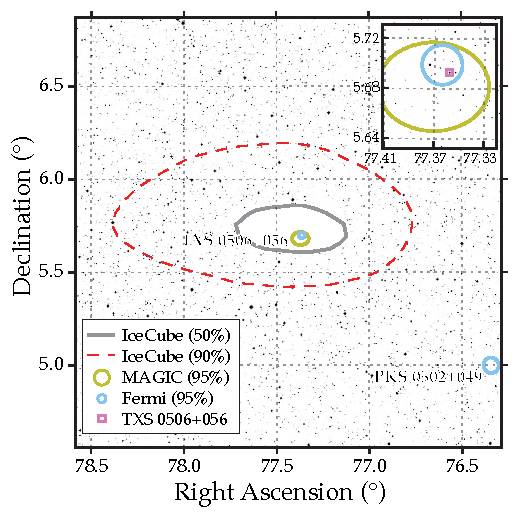
\includegraphics[width=1\textwidth]{theory/txs_localization.pdf}
    \end{subfigure}
    \begin{subfigure}[b]{0.52\textwidth}
        \centering
        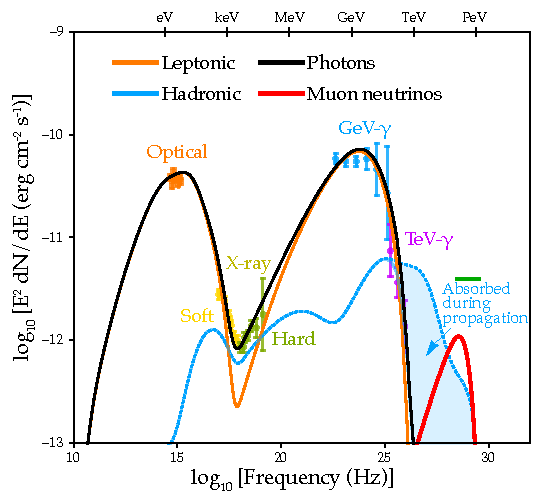
\includegraphics[width=1\textwidth]{theory/txs_modeling.pdf}
    \end{subfigure}
    \caption[\textit{TXS 0506+056}: Localization and SED]{Left: Localization of the flaring blazar \emph{TXS 0506+056}, found in coincidence with high-energy neutrino \emph{IC170922A}. The \SI{50}{\percent} (\SI{90}{\percent}) localization contours of the neutrino location are shown in grey (dashed red).\ Right: Hybrid lepto-hadronic emission model to explain the SED, including the detected high-energy neutrino. The leptonic component is shown as orange line, while the hadronic component is shown in blue. The resulting combined photon spectrum is displayed in black, and the muon neutrino spectrum in red. Adopted from~\cite{Aartsen2018, Gao2018}.}
    \labfig{txs}
\end{figure}

This lepto-hadronic model predicted a \SI{14}{\percent} probability of detecting a neutrino from the source without violating the bounds imposed by observations~\cite{Gao2018}. If one takes into account the large Eddington Bias~\sidecite{Strotjohann2019} expected for a single neutrino detection, this is still plausible. A consequence of this bias is that the neutrino flux of a single detection source could be systematically overestimated if that source is part of a large population emitting just below the IceCube detection limit, with occasional statistical overfluctuations.

However, producing the 2014--2015 neutrino flare without violating the gamma-ray limits proved to be a much harder challenge. No lepto-hadronic model\sidenote{To keep consistency with modeling the gamma-ray flaring state.} able to produce more than 2--5 neutrino events during the time period could be found~\sidecite{Rodrigues2019} without violating the observational constraints. It remains a challenge to reconcile both periods: The neutrino flux from the 2014--2015 period without a simultaneous gamma-ray flare on the one hand, and the single neutrino from 2017 accompanied by a gamma-ray flare on the other hand.

\subsubsection{Type II AGN \emph{NGC 1068}}
The second AGN-neutrino association was \emph{NGC 1068}. This active galaxy is located relatively nearby, with a distance of \SI{\sim14}{\mega\parsec}~\sidecite{Abbasi2022}. It was classified as Type II AGN, i.e.\ an AGN without signs of a jet and viewed relatively edge-on, with dust obscuring the SMBH and the BLR (see Section~\ref{agn})~\sidecite{Rosas2022}. It has an exceptionally high rate of star formation~\sidecite{Eichmann2016}, and hosts outflows~\sidecite{Cecil1990}. Due to these features, it had already been proposed as a production site of high-energy neutrinos in the 1970s~\sidecite{Silberberg1979}.

In 2022, an archival study comprising IceCube data from 2011 to 2020 found an excess of $79^{+22}_{-20}$ neutrinos with \unit{\tera\eV} energies from the location of \emph{NGC 1068}. This results in a neutrino luminosity between 1.5 and \SI{15}{\tera\eV} of $L_\nu = 2.9^{+1.1}_{-1.1}\times 10^{42}\,$\unit{\erg\per\s}, exceeding the equivalent gamma-ray luminosity between \SI{100}{\mega\eV} and \SI{100}{\giga\eV} by a factor of 18~\sidecite{Abbasi2022}.

\textit{NGC 1068} and \textit{TXS 0506+056} each contribute \SI{\sim1}{\percent} of the overall diffuse flux of astrophysical neutrinos measured by IceCube in their respective energy range. So far, it remains unclear if the diffuse flux is mainly composed of bright and nearby sources akin to \emph{NGC 1068}, a large population of faint sources with high redshifts ($z \geq 1$), or a mixture of both. Given the big difference in distance between \emph{NGC 1068} and \emph{TXS 0506+056}---the latter is about 100 times further away---and the differences in their respective spectra, it seems plausible to assume at least two distinct AGN source populations~\cite{Abbasi2022}.

\subsubsection{Gamma-ray Blazar Limits}
However, there are several constraints on the contribution from AGN\@. A stacking analysis from 2019 investigated 1301 gamma-ray blazars from 3FHL~\sidecite{Ajello2017}, the third catalog of hard gamma-ray sources issued by the \textit{Fermi} Large Area Telescope (LAT)~\sidecite{Atwood2009}. After stacking and searching for spatial correlations between through-going high-energy muon tracks from the northern hemisphere, no excess of neutrinos was detected~\sidecite{Huber2019}. Assuming a spectral source index of $\gamma=2$, an upper limit on the contribution of blazars to the high-energy neutrino flux between \SI{119}{\tera\eV} and \SI{4.9}{\peta\eV} was found: Not more than \SI{17}{\percent} of the diffuse flux can be attributed to these sources~\sidecite{Huber2019}.

\subsubsection{MeV Blazar Limits}
The contribution of MeV blazars was also tested. 137 blazars from the \textit{Fermi} Low Energy Catalog (1FLE)~\sidecite{Principe2018}, detected below \SI{100}{\mega\eV}, were stacked. The result was compatible with a non-detection. The upper limit derived from this---assuming a spectral index tracing the diffuse neutrino spectral index $\gamma=2.37$ and evaluated in an energy range between 30 and \SI{100}{\mega\eV}---was \SI{\sim1}{\percent} of the IceCube $\nu_\mu+\bar{\nu_\mu}$ flux~\sidecite{Abbasi_2022}.

\subsubsection{Jetted AGN Limits}

The correlation between high-energy alert neutrinos above \SI{200}{\tera\eV} with jetted (radio bright) AGN was also tested. The 3388 jetted AGN were selected from the Radio Fundamental Catalog\sidenote{\url{https://astrogeo.org/rfc}} by requiring X-band (\SIrange{8}{12}{\giga\Hz}) flux densities above 0.15 \unit{\jansky}. These were correlated with 56 published IceCube events with directional uncertainties below \SI{10}{\square\deg}. With these selections, a significant correlation was found, with a p-value of \SI{0.2}{\percent}~\sidecite{Plavin2020}.

However, a more recent study correlating this set of jetted AGN with the IceCube diffuse flux data comprising 10 years of muon tracks found no correlation~\sidecite{Abbasi2023a}. The unbinned maximum-likelihood-ratio method the study employed gave no significant correlation between the neutrinos and the jetted AGN, resulting in an upper limit on the overall contribution to the \unit{\tera\eV}--\unit{\peta\eV} neutrino flux of \SI{30}{\percent}.

Furthermore, a recent study correlating blazars in the southern hemisphere (as the earth's core gets opaque for neutrinos of the highest energies) from the Roma-BZCat Data Release 5 blazar catalog (5BZCat~\sidecite{Massaro2016}) with the 7-year all-sky map from IceCube found a correlation between blazars and high-energy neutrinos with a significance of $4.6~\sigma$. However, a follow-up study by IceCube was able to replicate the result, but when employing a 10-year neutrino all-sky map, the correlation vanished~\sidecite{Bellenghi2023}. This rather hints at a statistical fluctuation responsible for the 7-year map correlation.

\subsubsection{Non-jetted AGN Contribution}

The picture changes significantly when looking at non-jetted AGN: A recent study found a \SI{2.6}{\sigma} excess when correlating an infrared-selected subpopulation of non-jetted AGN with the astrophysical neutrino flux~\sidecite{Abbasi2022c}. The accretion disk luminosity of the AGN was estimated with their soft X-ray flux, and the source neutrino flux was weighted by that. The AGN population was selected based on the AGN radio emission and their infrared colors, and a \SI{2.6}{\sigma} excess (post trial) was obtained for this infrared-selected sample of 32,249 AGN.

\begin{marginfigure}
    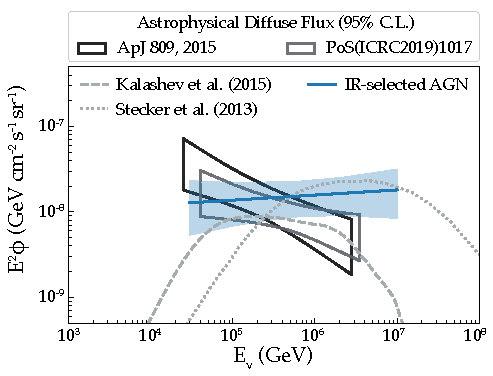
\includegraphics{theory/agn_ir.pdf}
    \caption[Non-jetted AGN]{Contribution of non-jetted AGN to the diffuse IceCube neutrino flux. The best-fit power law muon neutrino flux is shown in blue, corrected for completeness. Adapted from~\cite{Abbasi2022c}.}
    \labfig{agn_ir_contrib}
\end{marginfigure}

If this excess is interpreted as constituting a physical signal, it contributes $10^{+5}_{-4} ~\%$ of the diffuse flux at \SI{100}{\tera\eV}, see Fig.~\ref{fig:agn_ir_contrib}. Correcting for completeness, \SIrange{27}{100}{\percent} of the observed \SI{100}{\tera\eV} neutrinos could stem from particle acceleration within the accretion disks or coronae of AGN~\cite{Abbasi2022c}.

\subsection{GRB Limits}
GRB limits can be drawn from a search for a correlation between 807 GRBs detected during a period of three years with IceCube high-energy neutrinos during that time. The search was constrained to prompt emission (see Section~\ref{grb}) from GRBs, excluding precursor events or GRB afterglows. This was achieved by looking for cascade events in the detector (see Section~\ref{reconstruction}), which are created by neutrinos of all flavors. The neutrinos were required to be detected within the photon emission time as reported by the gamma-ray satellite for each GRB, the so-called prompt window. These prompt windows usually range from a few tens of seconds to a few minutes. Short windows are favorable for coincident searches, as the tight time-constraint strongly suppresses background events. Six events were found to be time-correlated with neutrinos, but also consistent with background. If they are interpreted as genuine signal events, GRBs contribute less than \SI{1}{\percent} to the diffuse neutrino flux~\sidecite[-33pt]{Aartsen2016a}.

An additional search extended the time window considered in order to search for a correlation between a subset of GRBs contained in \texttt{GRBweb}\sidenote{\url{https://user-web.icecube.wisc.edu/~grbweb_public/}} and over 7 years of IceCube data. Also with this expanded time window of \SI{1000}{\s} sensitive to parts of the GRB afterglow, no time correlation could be found, with an upper limit on the contribution to the diffuse flux of \SI{24}{\percent}~\sidecite{grb_ul}.

\subsection{Supernova Limits}
In 2023, a study~\sidecite{Necker2023} was published correlating $1040$ core-collapse SNe with 7 years worth of IceCube neutrino events. The SN data was obtained from the Weizmann Interactive Supernova Data Repository \texttt{WiseREP}\sidenote{\url{https://wiserep.org/}}~\sidecite{Yaron2012} and the Open Supernova Catalog~\sidecite{Guillochon2017}.

The study looked at correlations between individual supernovae, as well as the stacked full sample. Both methods yielded results that were compatible with the null hypothesis. In the study the SN neutrino energy spectrum was assumed to have a spectral index $\gamma=2.5$. Within the neutrino energy range of 1 to \SI{100}{\tera\eV}, the different types of SNe cannot contribute more than the following: SN IIP: \SI{59.9}{\percent}, SN IIn: \SI{33.9}{\percent} and stripped-envelope SNe (Ibc and IIb, see Section~\ref{sne}): \SI{14.6}{\percent}, assuming a choked-jet emission model~\cite{Necker2023}.

The first two classes were tested with a set of emission time windows, ranging between 100 and 1000 days after the first detection, while the stripped-envelope SNe were tested for choked-jet emission, in which the neutrinos would predate the optical emission (see Section~\ref{grb}). In this case, the time window started 20 days prior to, and ended with the first optical detection.\ Neither SNe IIn nor choked jet neutrino emission in stripped-envelope SNe can dominate the diffuse IceCube neutrino flux, while SNe IIP could still be dominant~\cite{Necker2023}.

\subsection{TDE Limits}
Lastly, there is a limit from stacking TDEs. A search comprising 13 non-jetted and 3 jetted TDEs, correlating with 9.5 years of IceCube muon neutrino data, found no significant excess. Under the assumption of constant TDE neutrino luminosity, upper limits for their contribution to the diffuse were derived. These constrain jetted TDEs to less than \SI{\sim1}{\percent}, and non-jetted TDEs to less than \SI{26}{\percent} of the diffuse flux detected by IceCube~\sidecite{Stein2019}.

\section{Conclusion}
The neutrino has been proposed, discovered and studied intensively. The detection of solar neutrinos, supernova neutrinos and finally the detection of a flux of high-energy neutrinos has firmly established the field of neutrino astronomy.

Nevertheless, the origin of the majority of the cosmic high-energy neutrino flux remains unclear. As can be seen in Fig.~\ref{fig:flux_ul}, no dominant source class has yet been established, though there are strong hints that non-jetted AGN contribute significantly to the diffuse neutrino flux. It is very much possible that the diffuse flux is composed of multiple source classes, each subdominant. The most stringent limits existing are those on prompt GRB emission and jetted TDEs, given their low rate density.

\begin{figure}[htb]
    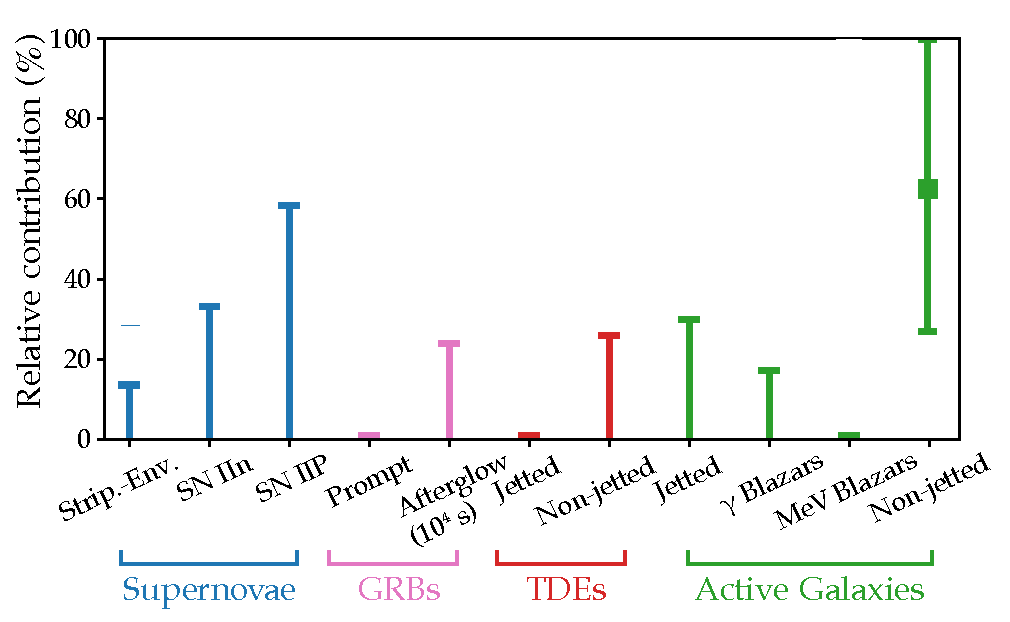
\includegraphics[width=1\textwidth]{theory/ul.pdf}
    \caption[Contribution to HE neutrino flux]{Potential source contributions to the diffuse IceCube high-energy neutrino flux. The values shown are mainly taken from~\cite{Guepin2022}, with some updates by the author. All numbers are discussed in the main text. Stripped-envelope SNe are denoted `Strip.-Env.' and a choked-jet emission model is assumed for these. Note that the unclear connection between the electromagnetic and expected neutrino flux, as well as uncertainties regarding the exact shape of the neutrino spectrum add significant uncertainties to these estimates. Adapted from a figure by Foteini Oikonomou.}
    \labfig{flux_ul}
\end{figure}

The absence of significant clustering of neutrinos, i.e.~the paucity of point sources in the data, disfavors the hypothesis that rare and luminous objects are responsible for the majority of the flux~\sidecite{Guepin2022}. It is entirely possible that the bulk flux stems from numerous faint objects, which could render establishing a dominant source class a challenging task.

\begin{marginfigure}
    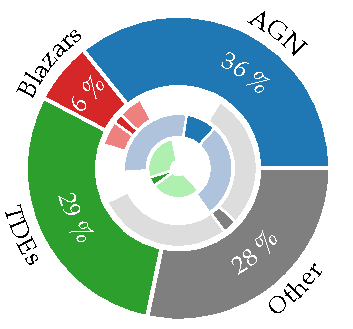
\includegraphics{theory/pie_chart.pdf}
    \caption[Neutrino flux contribution pie chart]{Pie chart of the contribution of known neutrino source classes as well as `other', comprising all source classes without association (main circle). The inner charts show the minimum (dark) and maximum (light) contributions within the \SI{90}{\percent} credible regions. Adapted from~\cite{Bartos2021}.}
    \labfig{pie_chart}
\end{marginfigure}

The flux could be fairly equally shared by AGN, TDEs and other sources, including blazars, as~\sidecite{Bartos2021} stipulate. The authors of that study estimated the contributions from source classes that have a known association (blazars: \emph{TXS 0506+056}, AGN: \emph{NGC 1068} and TDEs: \emph{AT2019dsg}) versus all other classes. They included statistical detection uncertainties accounting for the varying neutrino luminosity within source classes, as well as the redshift evolution of the number density and uncertainties of the detection process. The individual contributions are shown in Fig.~\ref{fig:pie_chart}, with the flux shared fairly equally between AGN, TDEs and other events, plus a noteworthy subdominant contribution by blazars.

Programs trying to establish a connection between individual high-energy neutrinos and sources within their localization are one good instrument in the available toolbox to solve the origin question at least partially. Such programs have the advantage of being time sensitive and allowing for follow-up observations necessary to classify ambiguous transients, contrary to archival studies. Chapter~\ref{fupipeline} will present one such program, a dedicated optical follow-up to high-energy IceCube neutrinos.

But first one needs to now how these two instruments work. The next two chapters will introduce the neutrino observatory IceCube (see Chapter~\ref{ic}) used in this study, as well as the optical facility (ZTF, see Chapter~\ref{ztf}).
\setchapterimage[7cm]{ic/ic_icecube_crop.jpg}
\chapter{The IceCube Detector}\label{ic}
\labch{IceCube}
One\marginnote{The IceCube Detector. Image credit: IceCube/NSF.} of the two most relevant instruments for this thesis is the IceCube Detector, a neutrino detector located at the geographic South Pole. It is the successor to the Antarctic Muon And Neutrino Detector Array (AMANDA) at the same location~\sidecite{Andres1999, Andres2000}.
\begin{marginfigure}
    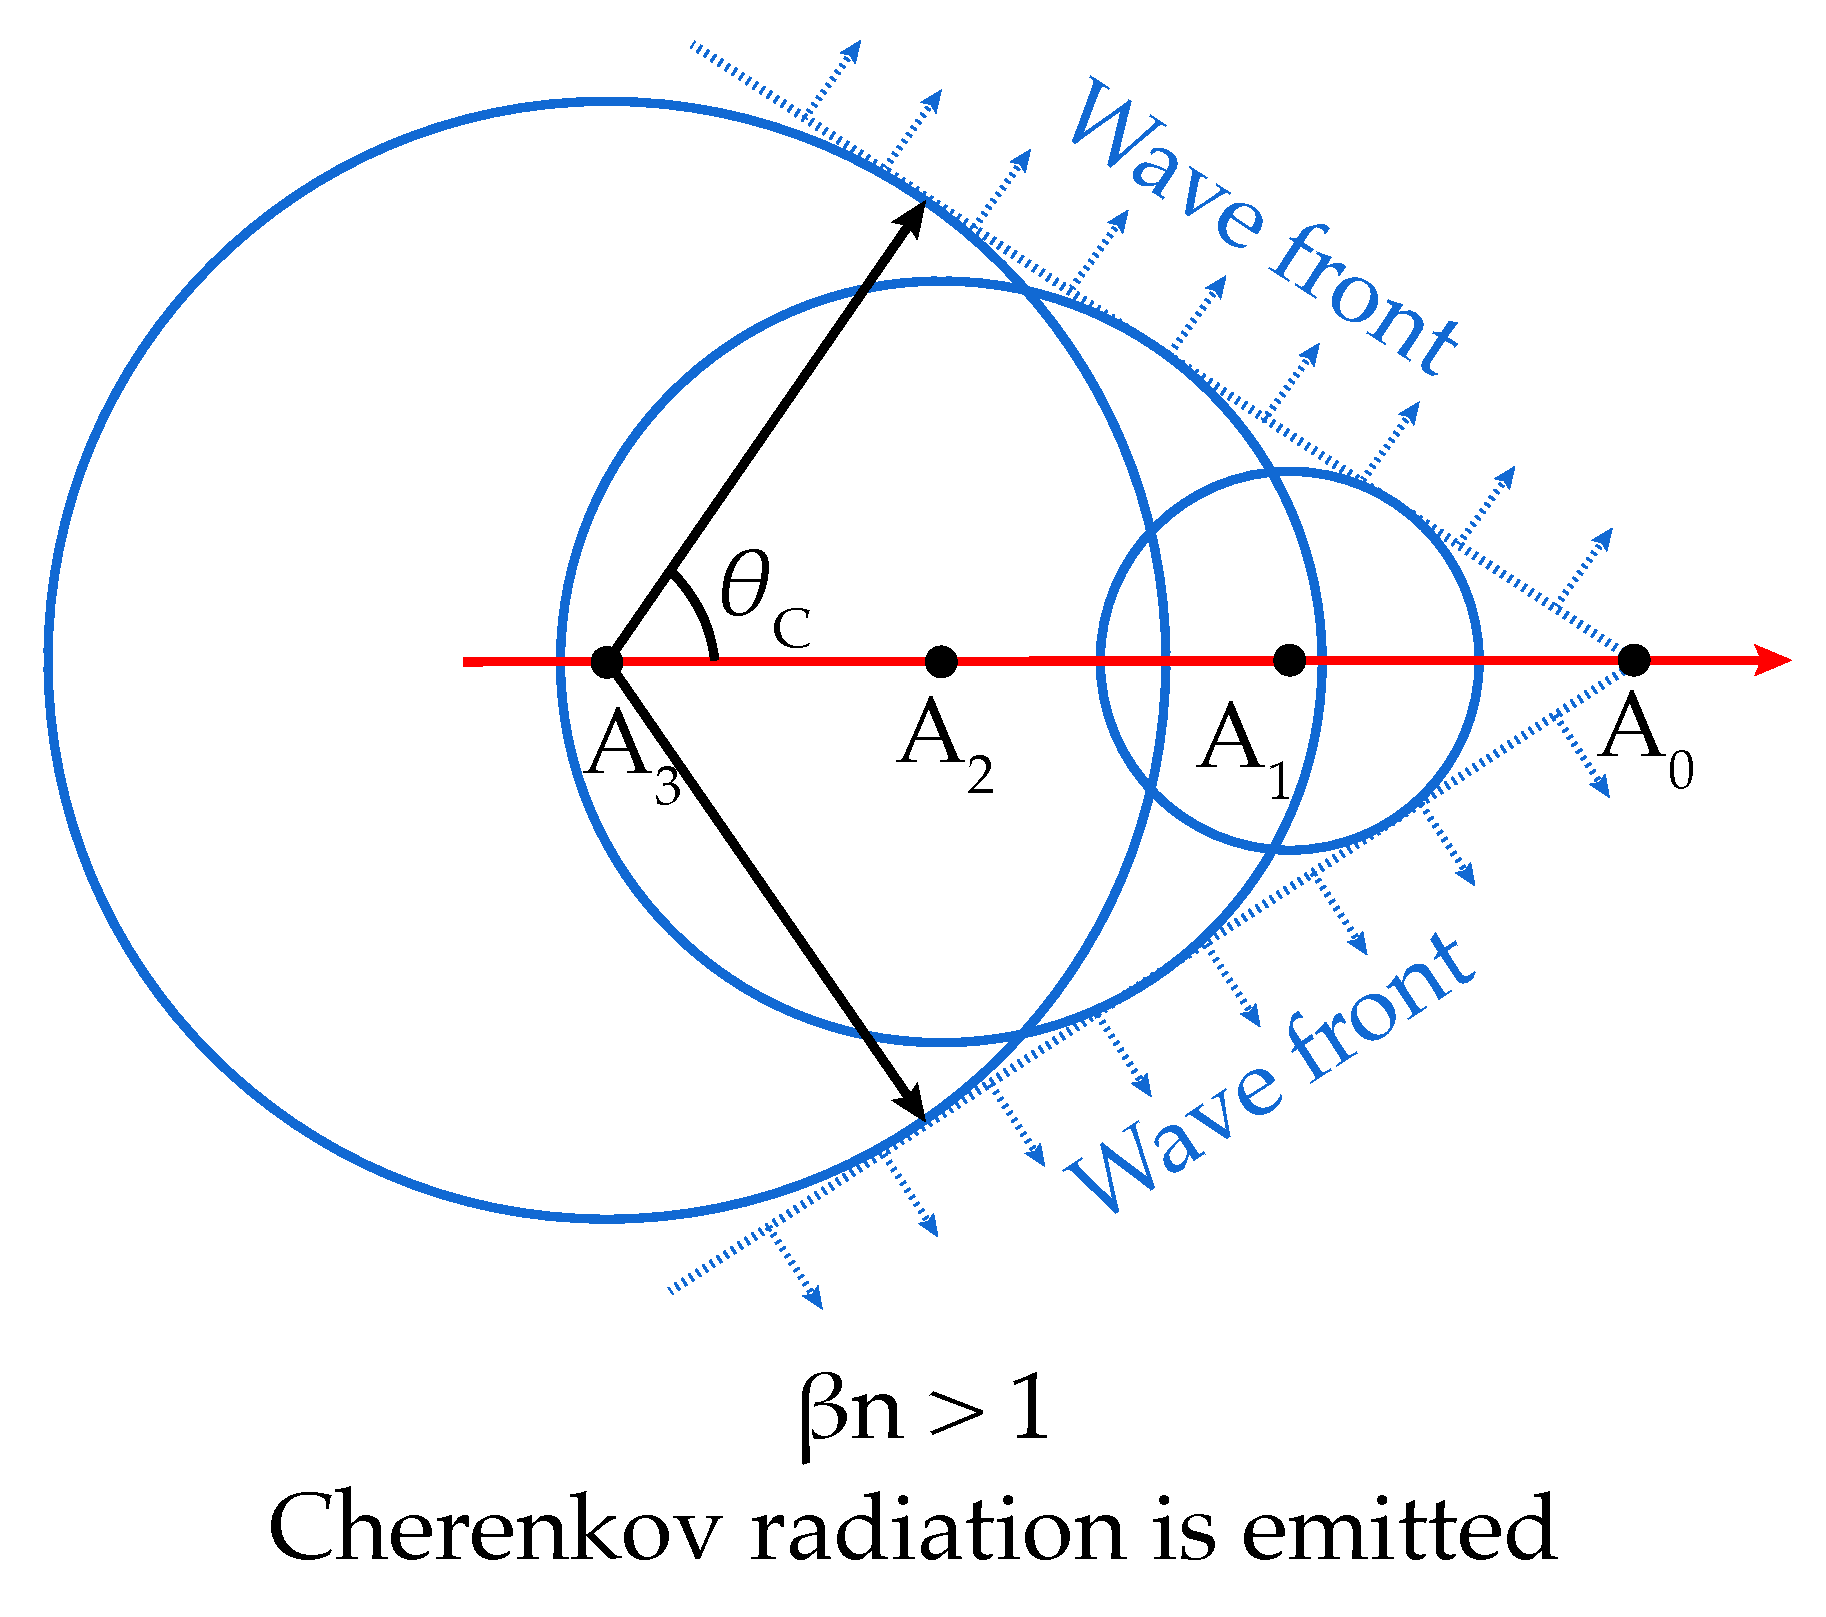
\includegraphics{ic/ic_cherenkov1.pdf}
    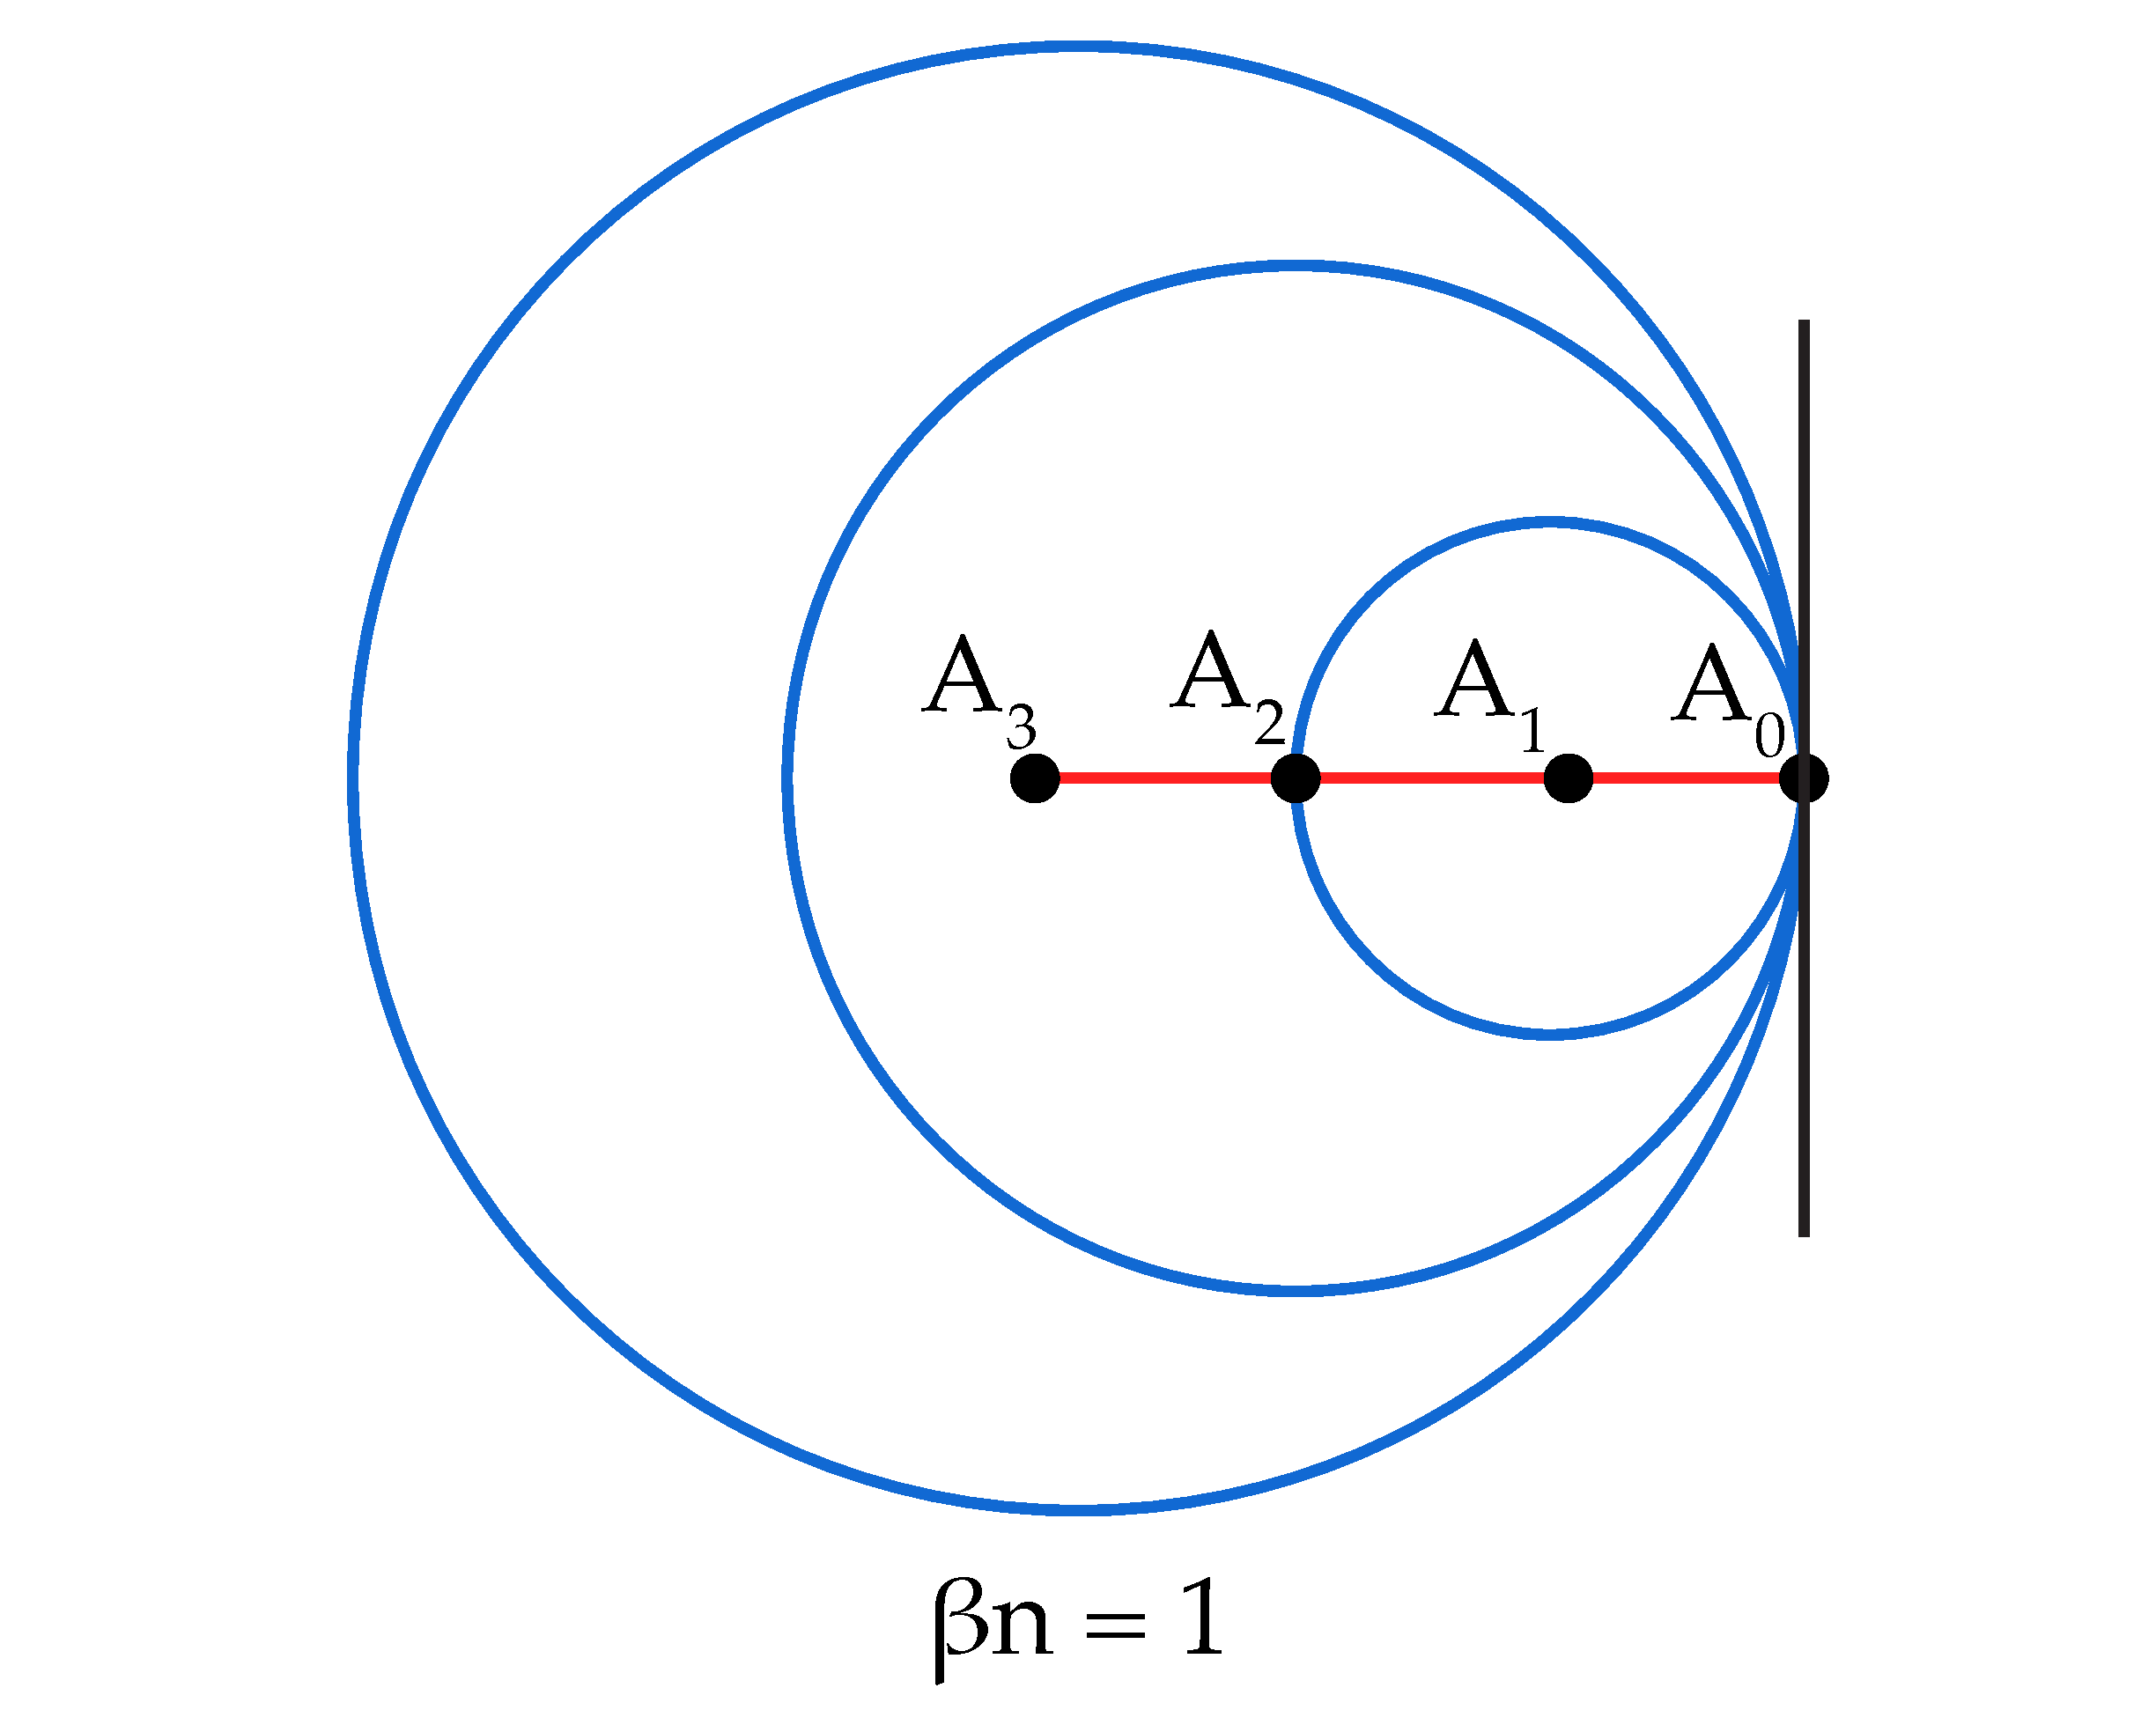
\includegraphics{ic/ic_cherenkov2.pdf}
    \caption[Cherenkov radiation]{The principle of Cherenkov radiation. In the upper figure Cherenkov radiation is emitted at the Cherenkov angle $\theta_\text{C}$, as the radiation emitted at different points in time forms a mutual, cone-shaped wavefront. In the figure on the bottom, all radiation is cancelled out by destructive interference (all circles are subsets of the first on the left, as the particle is not moving faster than light in the medium). Adapted from~\cite{LAnnunziata2020}.}
    \labfig{cherenkov}
\end{marginfigure}
The basic operational principle of IceCube (and already of AMANDA) is the detection of Cherenkov light within the Antarctic ice. When charged secondary particles created by neutrino interactions travel through the ice with an energy high enough, their speed can exceed the phase velocity of light in ice and they emit Cherenkov radiation. The detector consists of 5160 individual Digital Optical Modules (DOMs), buried deep in the ice and sensitive to the Cherenkov radiation.

\section{Cherenkov Radiation}\label{cherenkov_radiation}

Cherenkov radiation was first detected in 1934 by Soviet scientist Pavel Cherenkov~\sidecite{Cherenkov1934}. It occurs when charged particles travel within a medium with a velocity exceeding the speed of light in that very medium. The refractive index in a medium is defined as $n=\frac{c_0}{c_m}$, where $c_0$ is the speed of light in vacuum and $c_m$ is the phase velocity of light in that medium. Note that the phase velocity of light in a medium can exceed $c_0$, so $n<1$ is possible.

When charged particles cross an electrically neutral dielectric medium, atoms along the particle's path are briefly polarized. When they relax back to the ground state, the atoms emit electromagnetic radiation.

For non-relativistic particles, this radiation destructively interferes with itself, canceling out all signals (see the bottom panel of Fig.~\ref{fig:cherenkov}). But if the particle is traveling faster than the speed of light within the medium $c_m$, this destructive interference does not happen. Rather, a cone-shaped wavefront gets created (see top panel of Fig.~\ref{fig:cherenkov}). This wavefront constitutes Cherenkov radiation. If the particle has speed $v=\beta c_0$, the angle $\theta$ between the particle trajectory and the direction of the Cherenkov radiation can be calculated as~\sidecite{LAnnunziata2020}

\begin{equation}
    \cos{\theta} = \frac{\beta}{n}.
\end{equation}

If the medium is ice, to first order the refractive index $n$ is $\approx1.31$.\sidenote{This is of course rather crude. The $n$ of Antarctic glacial ice depends e.g.\ on depth; a fact we will come back to later when discussing directional reconstruction of high-energy IceCube neutrinos.} A secondary muon traveling through the ice at $0.999\,c_0$ will therefore emit Cherenkov light at an angle of $\theta = \cos^{-1}{\big(\frac{0.999}{1.31}\big)} \approx \SI{40}{\degree}$.
\begin{marginfigure}
    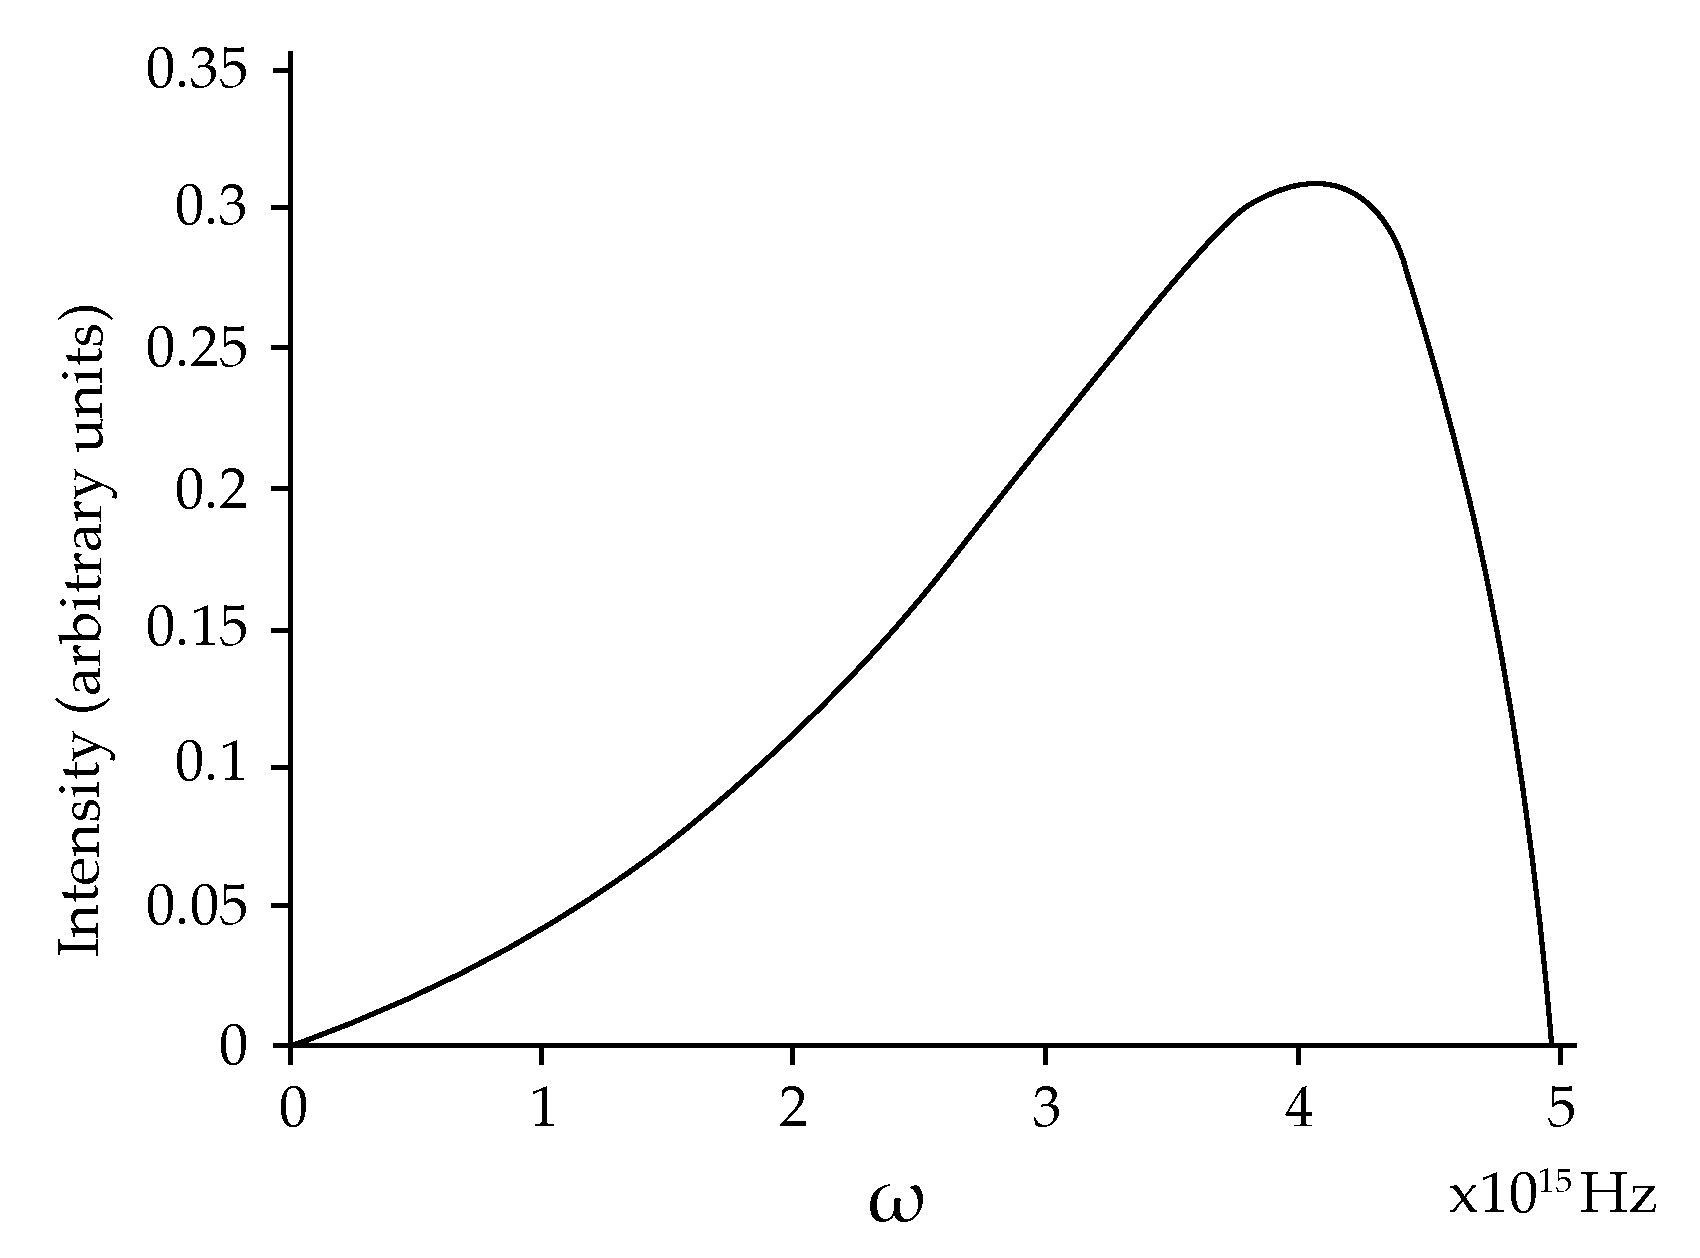
\includegraphics{ic/ic_cherenkov_spectrum.pdf}
    \caption[Cherenkov spectrum]{Cherenkov spectrum for a particle with $v=0.8 \,c_0$ in water. The intensity peaks at $\SI{4e15}{\Hz}$, corresponding to a wavelength of \SI{75}{\nm}, lying at the high-frequency end of the UV spectrum. Adapted from~\cite{Fulop1992}.}
    \labfig{cherenkov_spectrum}
\end{marginfigure}
Cherenkov radiation has a smooth spectrum, with a relative intensity roughly proportional to the frequency. Note that the refractive index of a medium also depends on the frequency, dropping below 1 in the X-ray. From this it follows that Cherenkov radiation appears blue to the human eye (the high-frequency part dominates) and its intensity peaks in the Ultra Violet (UV), before it sharply drops off in the X-ray regime~\sidecite{Fulop1992}, see Fig.~\ref{fig:cherenkov_spectrum}.

\section{Instrumentation}

IceCube detects neutrinos by observing the optical and UV part of their secondary particle Cherenkov spectrum (see Section~\ref{cherenkov_radiation} above). To understand how this is done, one first needs to look at the working principe of a Photomultiplier Tube (PMT), the basic instrument within the DOMs.

\subsection{Photomultiplier Tubes}
A PMT is a device used to detect very faint light signals by amplifying them. They consist of vacuum tubes and were successfully realized for the first time in the 1930s~\sidecite{Iams1935}.

\begin{figure}[h!]
    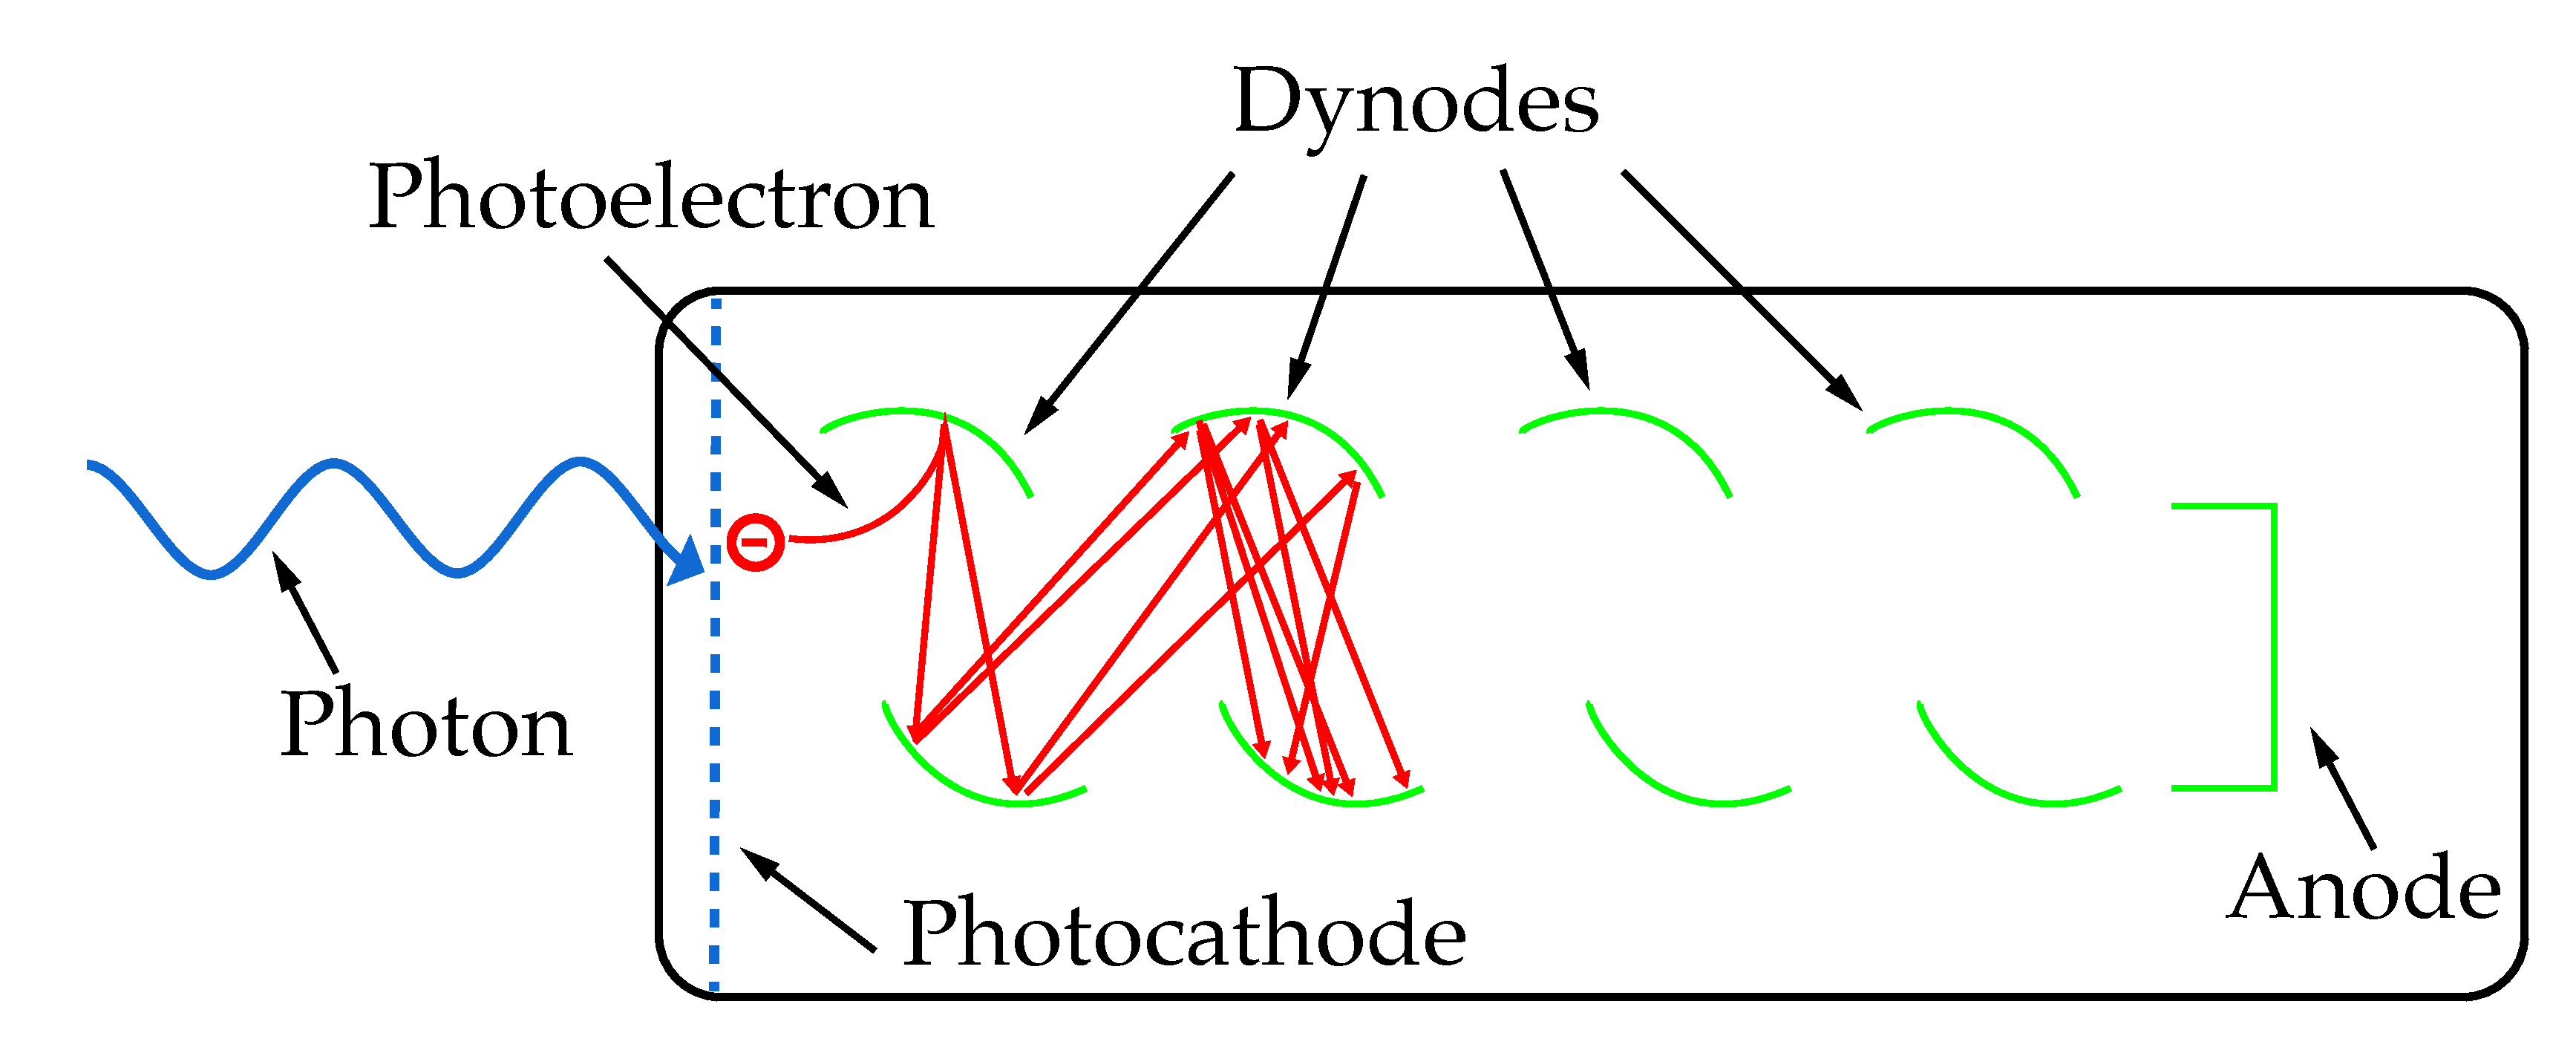
\includegraphics{ic/ic_pmt_annotated.pdf}
    \caption[PMT schematic]{A photomultiplier tube. Adapted from~\cite{Bednarski2014}.}
    \labfig{pmt}
\end{figure}

As one can see in Fig.~\ref{fig:pmt}, there are three principal components: a \textit{cathode}, several dynodes and an \textit{anode}. When photons hit the cathode, they can release electrons via the photoelectric effect~\sidecite{Einstein1905}. These photoelectrons are then accelerated (towards the right side in Fig.~\ref{fig:pmt}) by an electric field within the tube. This field is generated by applying a high voltage between the cathode and the anode.

To amplify the signal, a number of dynodes are placed between cathode and anode. These are additional electrodes with subsequently higher voltages. When the photoelectron hits the first dynode, a number of secondary electrons are generated, which are then accelerated towards the next dynode by the electric field. This process repeats for every dynode, generating an electron avalanche exponentially amplifying the original single photoelectron signal. The number of secondary electrons hitting the anode is proportional to the number of incident photons, resulting in a linear detector response (as long as the detector stays below its saturation limit)~\sidecite{Wright2017}.

IceCube uses PMTs made by Hamamatsu Photonics (R7081--02), sensitive to photons between 300 and \SI{650}{\nm}. They have a quantum efficiency (QE) at \SI{390}{\nm} of \SI{25}{\percent}, are operated with a voltage of \SI{1500}{\V} and have a gain (electron multiplication factor) of \num{e7}. The photon-sensitive surface area is typically \SI{530}{\cm\squared}~\sidecite{Abbasi2010}.

\subsection{The Digital Optical Module}\label{DOM}
\begin{marginfigure}
    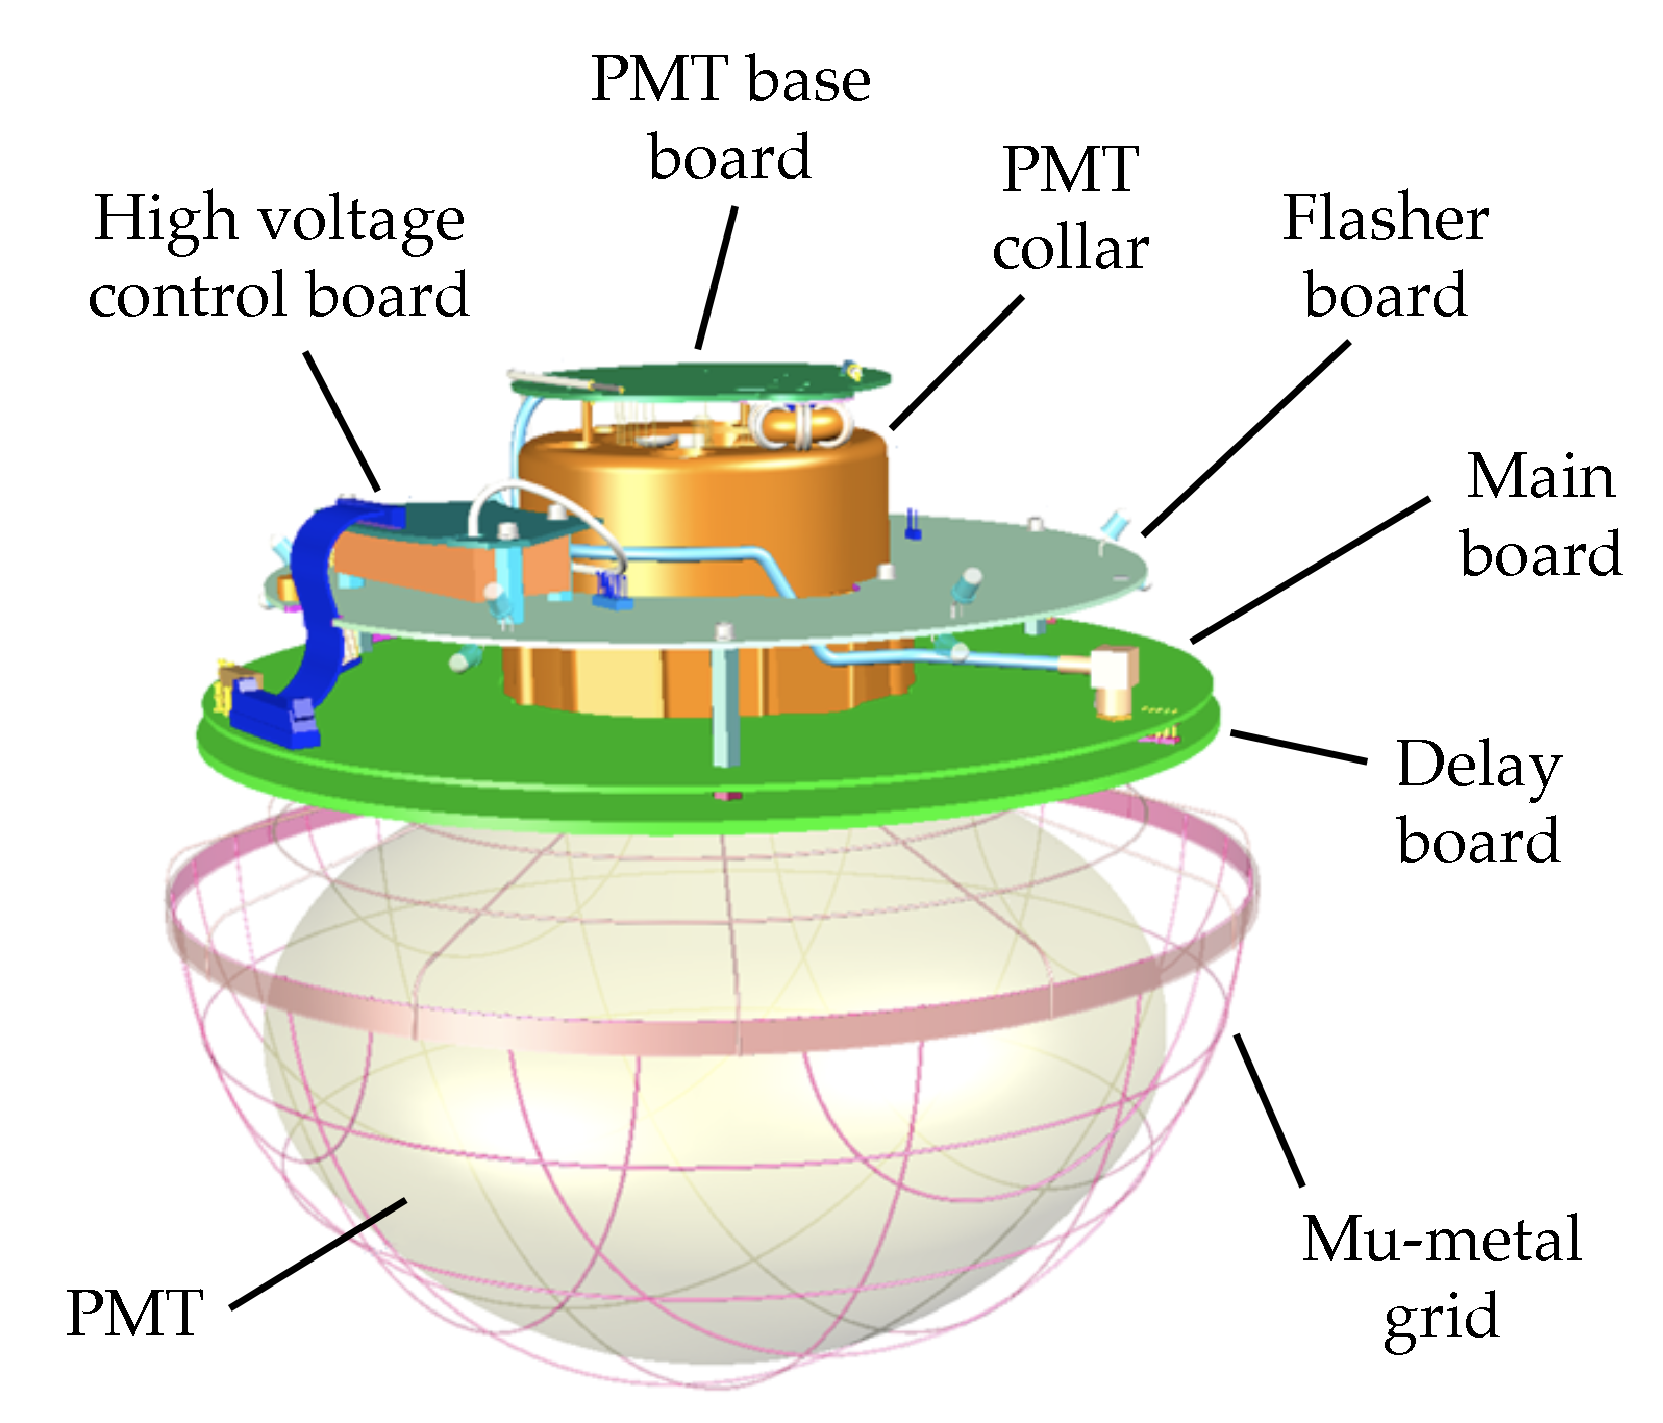
\includegraphics{ic/ic_DOM.pdf}
    \caption[IceCube digital optical module]{The IceCube DOM seen from the side. The detecting side of the PMT is facing downwards, with the main board and the PMT base board on top. From~\cite{Aartsen2017}.}
    \labfig{ic_dom}
\end{marginfigure}

The individual IceCube PMTs for detecting the Cherenkov radiation are enclosed in the DOMs. Each DOM consists of a pressure-resistant glass sphere, several controller boards and the PMT, facing downward (see Fig.~\ref{fig:ic_dom}). The glass sphere can withstand long-term pressure of \SI{250}{\bar}. The optical transmission of the spheres was measured to be \SI{93}{\percent} at \SI{400}{\nm}, decreasing to \SI{10}{\percent} at \SI{315}{\nm}.

The circular main board hosts data acquisition and control systems, as well as units for communication and a power converter. Another board interfaces with the PMT, while additional boards delay the PMT signals and generate the high voltage current powering the PMT. Additionally, there is a so-called \textit{Flasher Board} that controls Light-Emitting Diodes (LEDs). These are used to generate light flashes which can be received by neighboring DOMs for calibration purposes~\sidecite{Aartsen2017}.

\begin{marginfigure}
    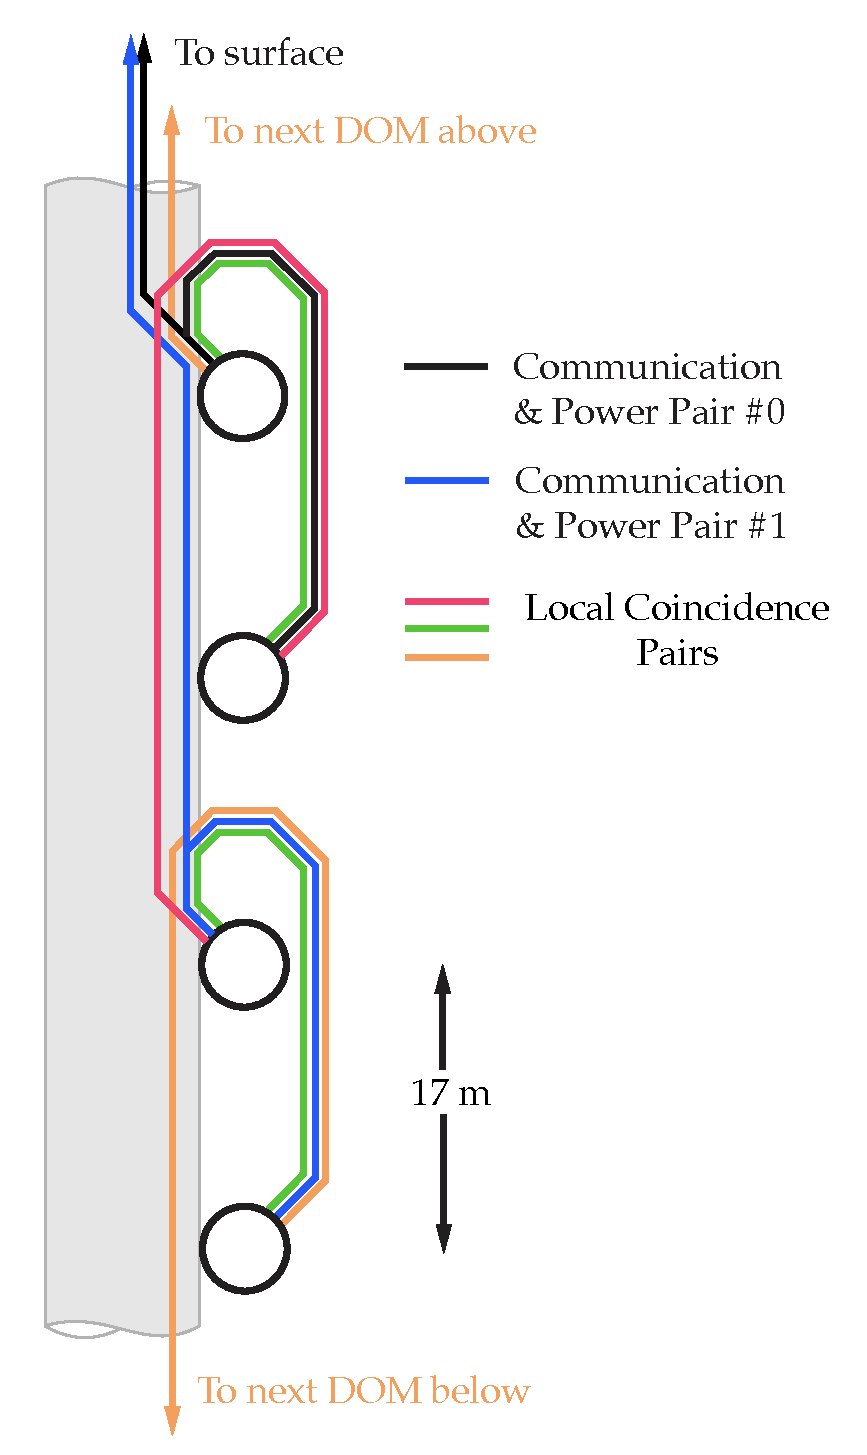
\includegraphics{ic/ic_DOM_connections.pdf}
    \caption[IceCube DOM connections]{Connection scheme for four IceCube DOMs along one string. Pairs of DOMs share one twisted-pair cable. Also, each DOM is directly connected to its direct neighbors above and below. Adapted from~\cite{Aartsen2017}.}
    \labfig{ic_dom_connections}
\end{marginfigure}

Because of data storage restrictions, the DOMs only record and digitize the photon signal after several trigger criteria have been met. The digitized voltage over time detected by the PMTs is called a waveform, and combined with a timestamp it comprises the basic datum in IceCube, a hit.

To fully record the waveform after a hit, the signal needs to be stored in a buffer. This is realized with the delay board, which routes the analog PMT signal through a \SI{10}{\m} long, serpentine copper trace to delay it by \SI{75}{\ns}.

When a hit is detected, the DOM sends a tag signal to the neighbor and next-to-nearest neighbor DOMs. When no neighbors detect a hit, the isolated hit only contains the timestamp, the amplitude and charge information extracted from the waveform. When at least two neighboring DOMs also detect a hit within \SI{0.25}{\micro\s}, a Local Coincidence (LC) is triggered. If the signal passes a threshold of 0.25 photoelectrons, the recorded waveforms are digitized and appended to the hits tagged as LC~\cite{Aartsen2017}.

The digitization of the PMT waveform is done with the Analog Transient Waveform Digitizer (ATWD), a custom-built Application Specific Integrated Circuit (ASIC). Usually lying dormant, the ATWDs start to capture the delayed waveform when the PMT discriminator initiates it. The captured waveforms are only digitized in case a hit (i.e.\ local coincidence) is registered~\cite{Aartsen2017}.

The DOMs are connected to the IceCube Laboratory (ICL) with twisted-pair copper cables. The power for the DOM is also transmitted with this cable. Two DOMs share one twisted-pair cable, and each DOM is also directly connected to its two neighbors on the same string. Fig.~\ref{fig:ic_dom_connections} shows the connection layout.

The Flasher Board houses 12 LEDs operating at \SI{\sim400}{\nm} wavelength. These are used to verify the DOM timing response, to measure the DOM in-ice position, to determine the optical properties of the ice, and to verify the reconstruction algorithms~\cite{Aartsen2017}.

\subsection{Detector Layout}
In total, approximately 5800 DOM units were built and tested, 300 failing tests and the rest being delivered to the South Pole. The vast majority of these were ultimately deployed (5160 in total). The final detector layout (since the last drilling campaign 2010/2011, see below) consists of 86 strings. The DOMs were deployed along those strings, like pearls on a necklace. Each string contains 60 DOMs, with an average horizontal spacing between strings of \SI{125}{\meter}~\cite{Aartsen2017}.

\begin{figure}
    \includegraphics[width=1.\textwidth]{ic/ic_side_view_font.pdf}
    \caption[IceCube side-on]{Side view of the IceCube detector, showing the instrumented array deep in the Antarctic glacial ice. In the center on top is the IceCube Laboratory, were data processing takes place. From~\cite{Ahlers2018a}.}
    \labfig{ic_sideon}
\end{figure}
\begin{marginfigure}
    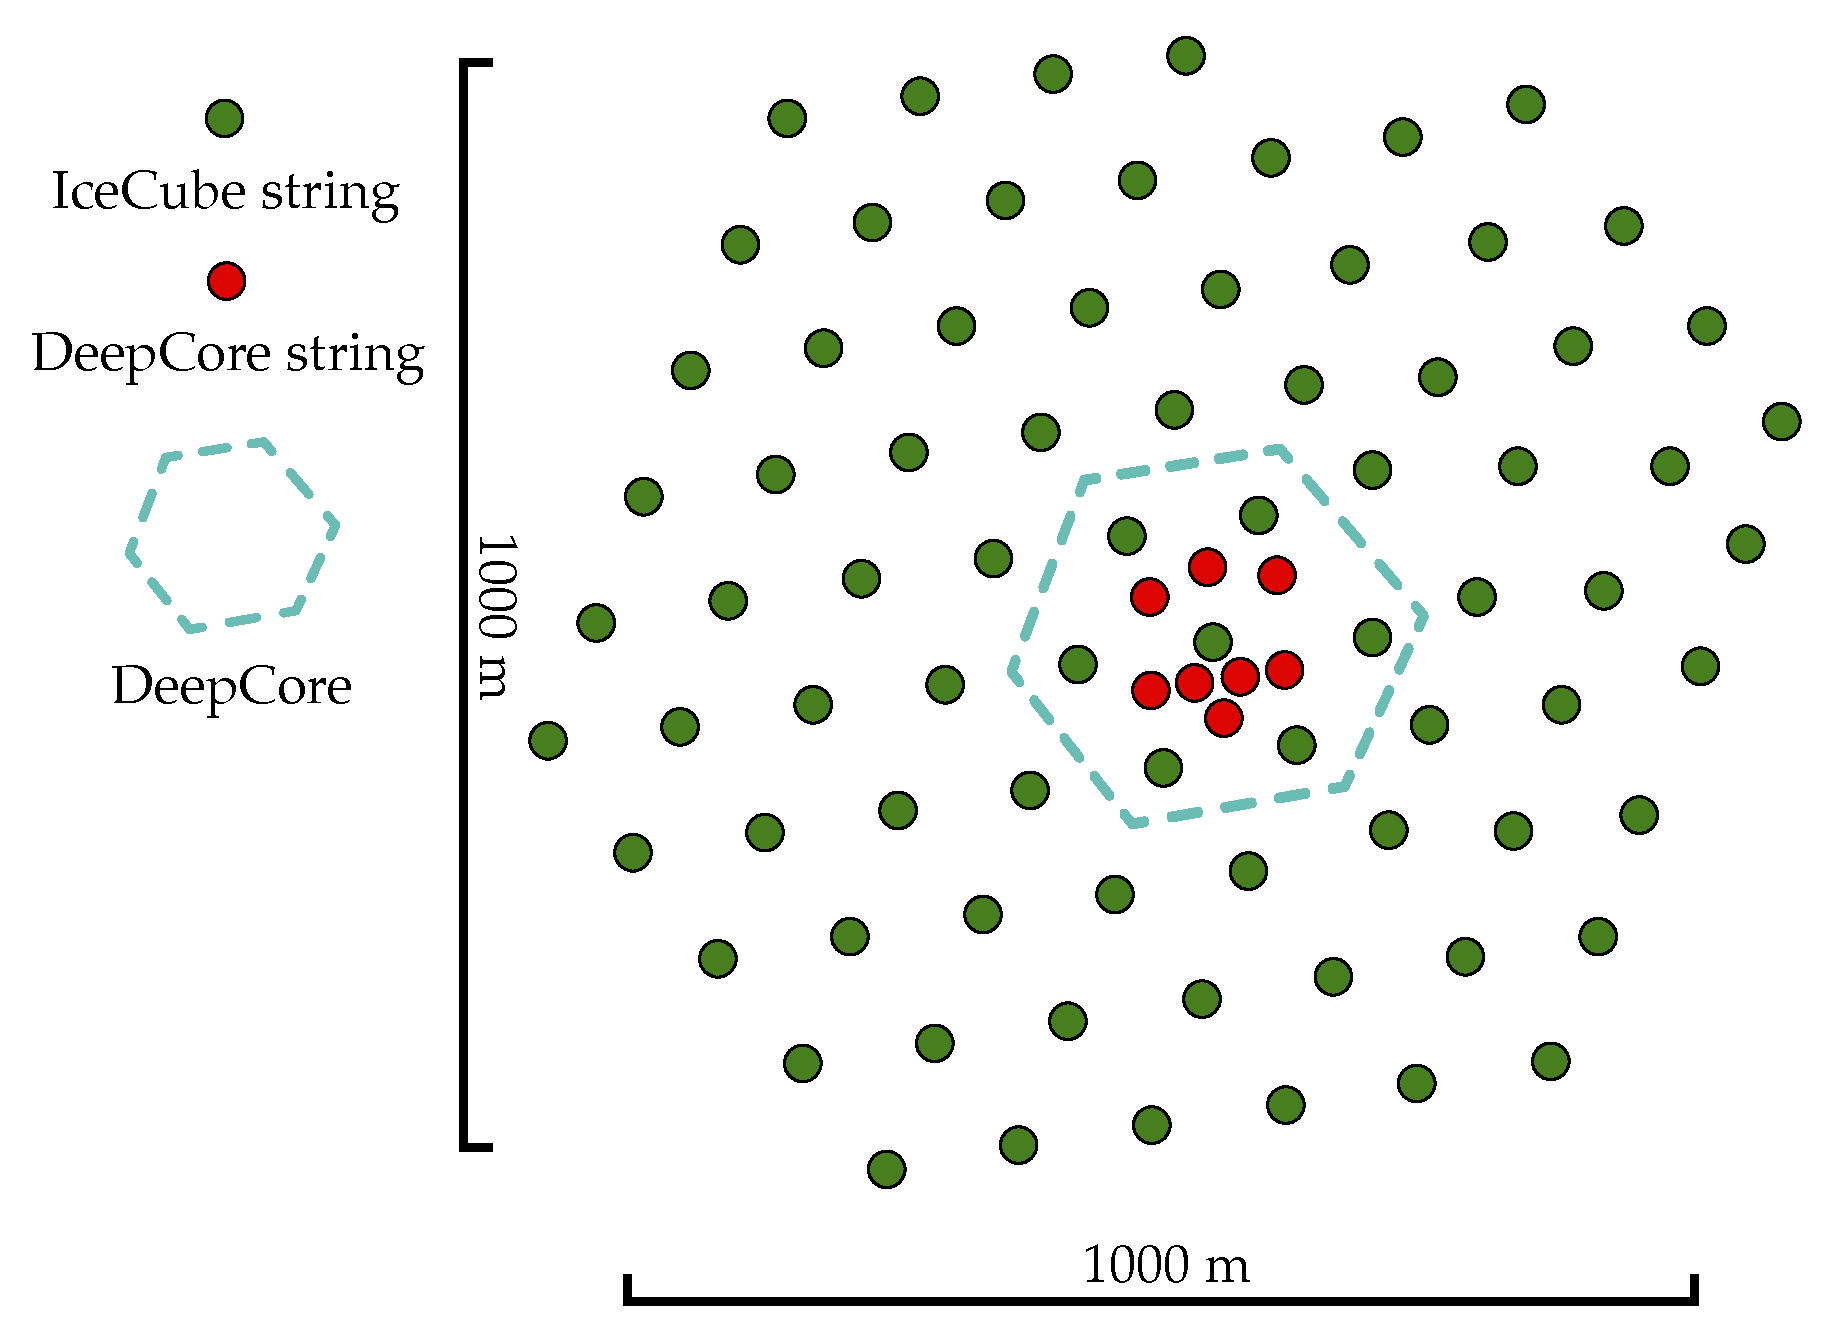
\includegraphics{ic/ic_top_view.pdf}
    \caption[IceCube top-down view]{Top-down view of the IceCube detector, spanning \SI{1}{\square\km} on the surface. From~\cite{Ahlers2018a}.}
    \labfig{ic_top_down}
\end{marginfigure}

The instrumented part of the strings starts at \SI{1450}{\m} below surface, with one DOM every \SI{17}{\m} to a depth of \SI{2450}{\m}, just above the bedrock at a depth of \SI{2820}{\m}. In Fig.~\ref{fig:ic_sideon} the layout of the in-ice array can be seen. The strings follow a roughly hexagonal layout (see Fig.~\ref{fig:ic_top_down}), with a side length of \SI{1}{\km\squared}. The total instrumented volume of glacial ice is thus \SI{1}{\km\cubed}~\cite{Aartsen2017}. Of the 5160 deployed DOMs, 92 are dead as of March 2023, a loss of \SI{1.7}{\percent}\sidenote{This is better than the predicted failure percentage, which was projected to be \SI{2}{\percent} by 2023~\cite{Aartsen2017}.}.

One can see in Fig.~\ref{fig:ic_top_down} that there is a region in the center of the detector which is more densely instrumented: The strings are closer to each other, and also the spacing between DOMs on these strings is reduced from \SI{17}{\m} to \SIrange{7}{10}{\m}. This part of the detector is DeepCore, designed to have a lower energy threshold of \SI{10}{\GeV}, a significant improvement over the \SI{100}{\GeV} for the rest of the detector. The DOMs within DeepCore are also modified for this goal, as they are equipped with PMTs that have a \SI{35}{\percent} higher QE compared to the `normal' DOMs~\cite{Aartsen2017}.


\subsection{Deployment}
As one can imagine, embedding the DOMs within the ice was a non-trivial task. It required drilling 86 boreholes with a diameter\sidenote{The hole diameter was larger than the DOM diameter (\SI{35}{\cm}) to account for partial refreezing of the bore hole.} of roughly \SI{60}{\cm} and a length of \SI{2500}{\m}. This was achieved over several drilling campaigns with the Enhanced Hot Water Drill (EHWD) specifically built for this task. This drill had a total power of \SI{5}{\mega\W} and was able to drill with a maximum speed of \SI{2.2}{\meter\per\minute}. With these performance characteristics, one hole was drilled every \SI{48}{\hour} on average\sidenote{Drill operation happened around the clock.}~\cite{Aartsen2017}. It took 7 drilling seasons to deploy the final IceCube86 setup, from the Antarctic summers 2004/2005 to 2010/2011. Fig.~\ref{fig:ic_drill} shows the tower operations site directly above the bore hole~\sidecite{Benson2014}.

The water for drilling the holes was heated to \SI{88}{\celsius} with 35 water heaters working in parallel, each providing \SI{125}{\kilo\W} power. The average amount of fuel used per drill hole was \SI{27000}{\liter}~\cite{Benson2014}.

\begin{figure}[]
    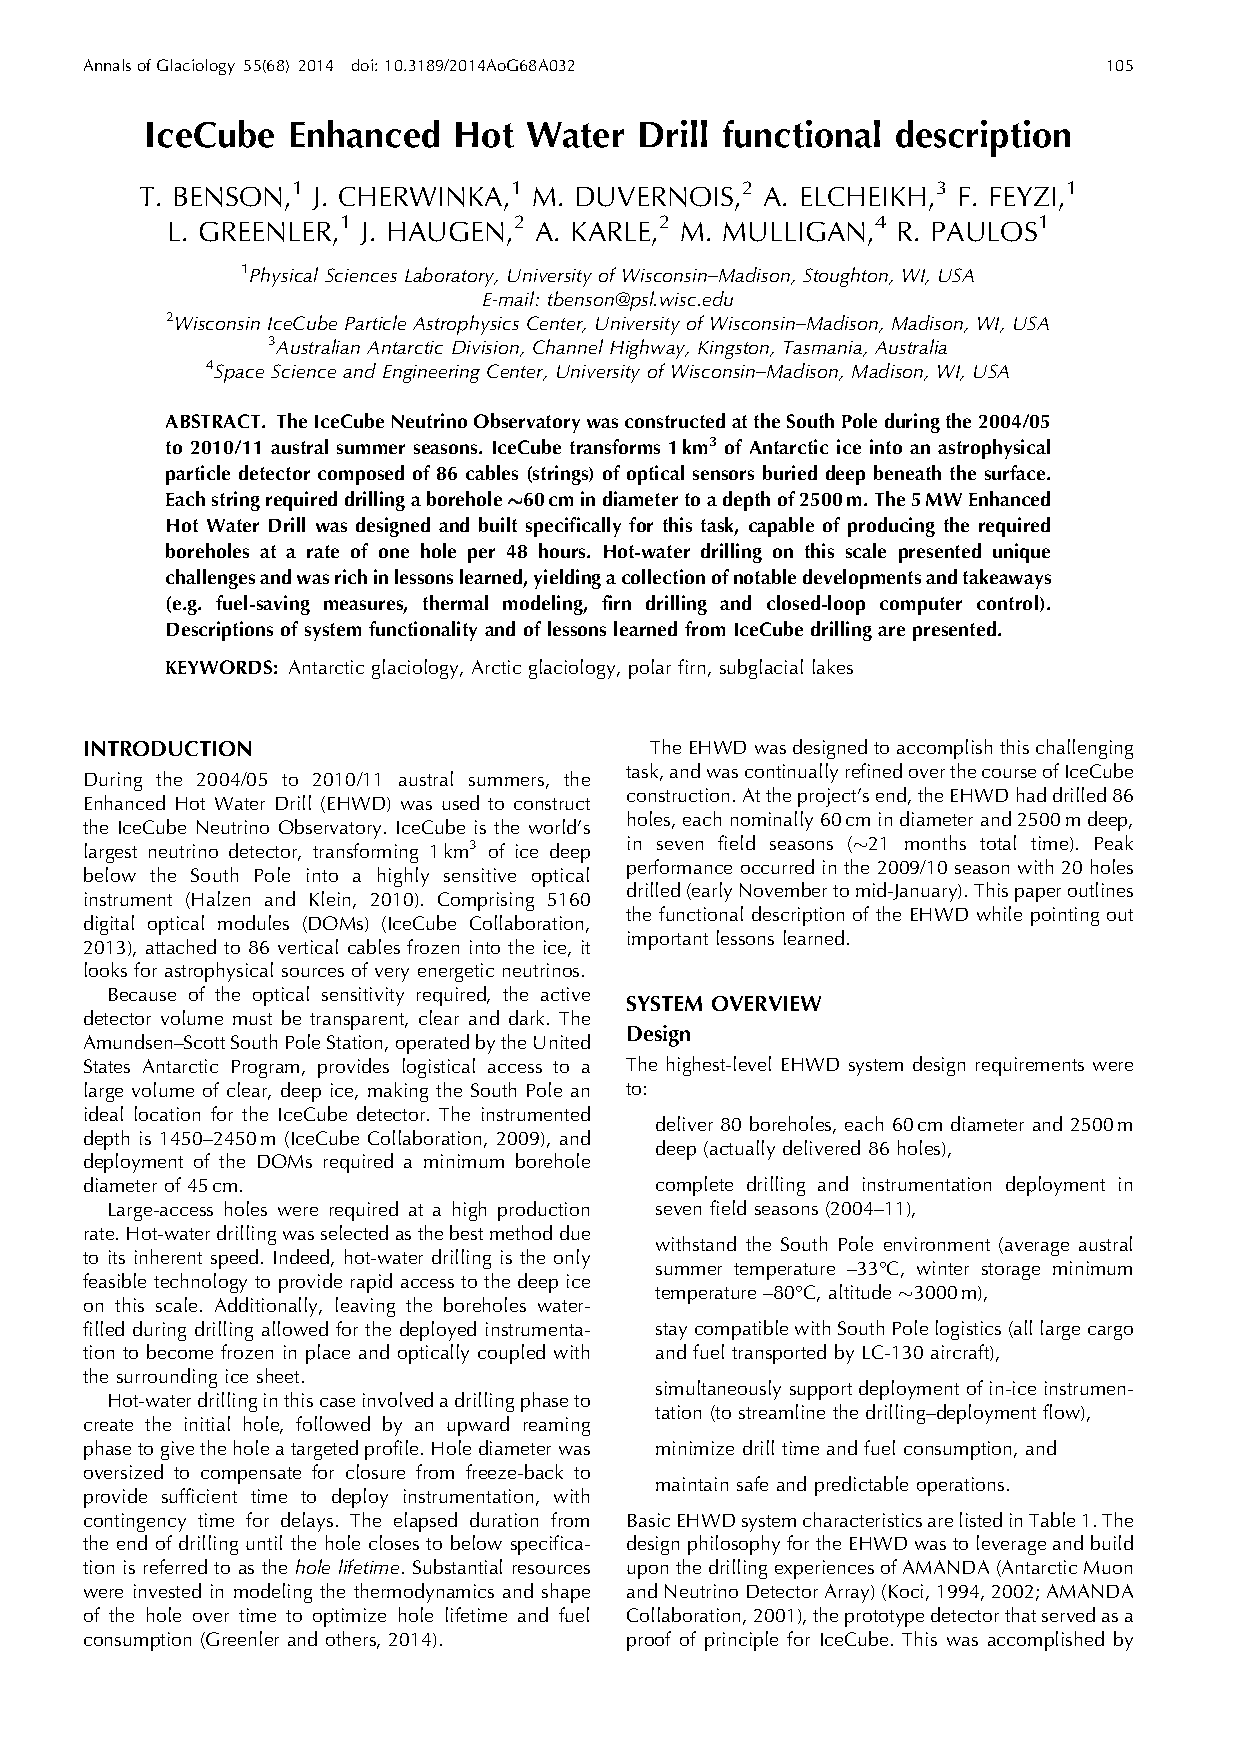
\includegraphics{ic/ic_drill.pdf}
    \caption[IceCube enhanced hot water drill]{The hole drilling part of the IceCube Enhanded Hot Water Drill, excluding the hot, pressurized water supply. One can see the tower operations site (TOS) above the hole and the hoses providing hot water and returning cooled water from the bore hole to the generators in a closed loop. From~\cite{Benson2014}.}
    \labfig{ic_drill}
\end{figure}

\subsection{The IceTop Surface Array}

\begin{marginfigure}
    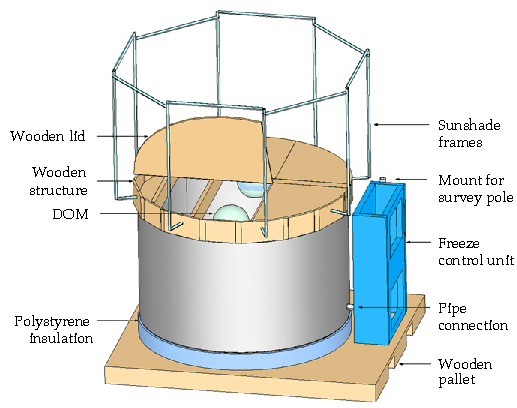
\includegraphics{ic/ic_icetop.pdf}
    \caption[IceTop detector]{IceTop surface Cherenkov detector tank. From~\cite{Abbasi2013}.}
    \labfig{ic_icetop}
\end{marginfigure}

In addition to the in-ice detector, IceCube has a surface air shower detector for cosmic-ray physics\sidenote{See Section~\ref{cosmic_rays}.}, named IceTop. It was designed to study the cosmic-ray mass composition by correlating the energy it measures on the surface with the energy deposited by muons in the ice as measured by the in-ice detector~\sidecite{Abbasi2013}. The energy sensitivity range of IceTop is \SI{300}{\tera\eV} to \SI{1}{\exa\eV}~\sidecite{Aartsen2013a}.

The IceTop surface array consists of $2\times81$ ice-filled Cherenkov tanks. These are placed in pairs on the same hexagonal grid as the DOM strings for the in-ice array. Each tank is equipped with two standard IceCube DOMs (see Section~\ref{DOM})~\cite{Abbasi2013} which are operated at two different gain levels to increase the dynamic range.

Results from 3 years of IceTop data show good agreement between models describing the transition from galactic to extragalactic cosmic rays at energies above the knee. In these, the spectrum of lighter elements softens earlier towards higher energies compared to heavier elements. This is indeed reflected in the data~\sidecite{Aartsen2019}.

Furthermore, IceTop can be used to increase the purity of a sample of astrophysical neutrinos by using it to veto muon events that mostly stem from cosmic-ray induced air showers, as opposed to muons created by neutrino interactions~\sidecite{Amin2021} (more details on background rejection will follow in Section~\ref{background}).

\subsection{Data Acquisition}\label{data_acquisition}
As noted above, only for locally coincident hits in multiple detectors the full waveforms are digitized by the DOMs. These are then sent to the IceCube Laboratory on the surface via the twisted-pair cable datalink, were all DOM data is ingested into the data acquisition system (DAQ). Hits throughout the detector are investigated by the system to establish common causility by temporal and sometimes spatial patterns. All hits for which common causality can be established form an event. The rate of these events varies seasonally with the atmospheric muon flux, with a median event rate of \SI{2.7}{\kilo\Hz} and a total data rate of \SI{1}{\tera\byte\per\day} (roughly \SI{100}{\mega\bit\per\second})~\cite{Aartsen2017}.

Satellite bandwidth is limited and costly. Therefore, further on-site software triggers reduce the data rate to \SI{15}{\percent} of the initial rate. These events are then transmitted via satellite to the IceCube data center at the University of Wisconsin-Madison for further analysis. The full event stream is also written to redundant disks, which are transferred twice per year to Madison.

\subsection{Time Synchronization}
Precise timing information is crucial to reconstruct an event (see Section~\ref{reconstruction}). For this reason, all DOMs need to be synced to a common clock. This is achieved by syncing the whole system to a Symmetricom ET6000 GPS receiver. The synchronization of individual DOMs is performed once per second, while data transfer is paused during the process\sidenote{The calibration sequence takes $\lesssim$\SI{1.3}{\milli\second}}~\sidecite{Abbasi2009}.

IceCube ensures temporal synchronizity with an algorithm called Reciprocal Active Pulsing (\texttt{RAPcal}): A bipolar pulse is initiated on the surface and sent to the DOM. The sender saves the local time when it sends the pulse and starts a timer. Upon reception down the string, the DOM also saves its current local time, saves the received pulse waveform, starts a timer, responds with a bipolar pulse of its own and stops the timer. Upon reception, the surface station stops its timer and requests the received pulse waveform and all timing information from the DOM.

With these six pieces of information --- the two transmit timestamps, the two receive timestamps and both waveforms --- a transformation from the GPS-synchronized surface to local DOM time domain and vice versa can be calculated, with a precision of \SIrange{1}{2}{\ns}~\cite{Abbasi2009}.

\section{Angular Reconstruction}\label{reconstruction}

The goal of IceCube reconstruction is twofold: Reconstructing the deposited neutrino energy, and reconstructing the neutrino arrival direction. With this in mind, one can sort the events seen by the detector broadly into two categories: Well localized track events with poorly reconstructed energy, and cascade events with well-determined energy, but very imprecise origin.

\subsection{Event Types}\label{ic_event_types}

\begin{marginfigure}
    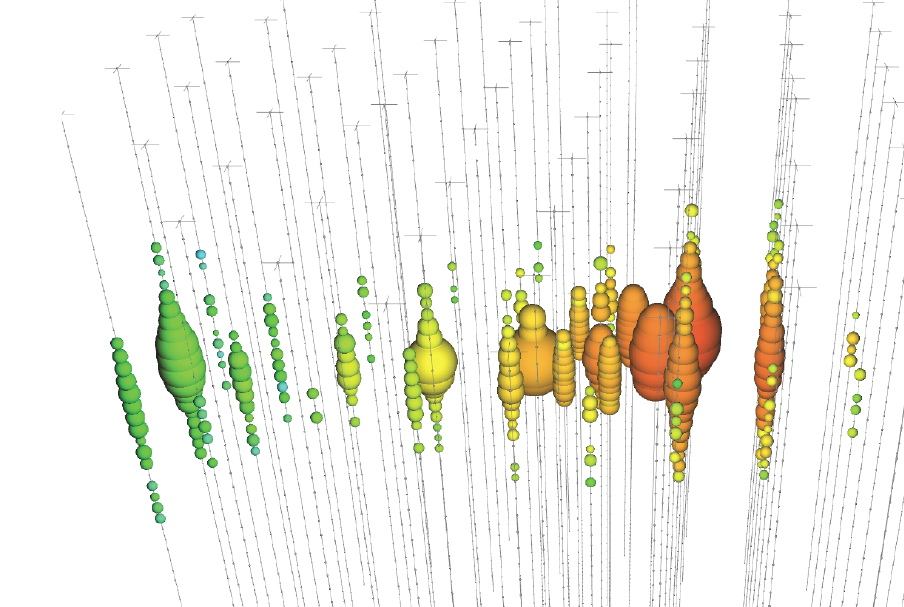
\includegraphics{ic/ic_track.png}
    \caption[Track event in IceCube]{Cascade event: The long track allows for good angular reconstruction, with high uncertainty on the event energy. From \url{masterclass.icecube.wisc.edu}.}
    \labfig{ic_track}
\end{marginfigure}
\begin{marginfigure}
    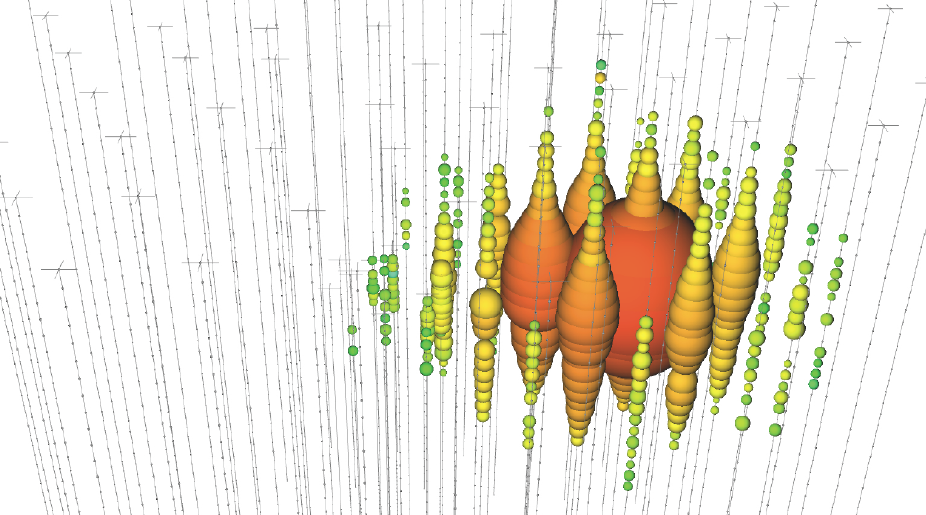
\includegraphics{ic/ic_cascade.png}
    \caption[Cascade event in IceCube]{Cascade event: The energy is fully contained in the detector, as the event is relatively isotropic. The angular uncertainty is quite large though. From \url{masterclass.icecube.wisc.edu}.}
    \labfig{ic_cascade}
\end{marginfigure}
\begin{description}
    \item[Track Events] (Fig.~\ref{fig:ic_track}) are produced by secondary muons resulting from the charged-current interaction of muon neutrinos with the Antarctic glacial ice (see section~\ref{neutrinos_current}). The secondary muons leave tracks in the ice with a length on the order of kilometers. Muons with energies above \SI{\sim300}{\giga\eV} create tracks that exceed the detector length. In general, this allows for a good angular resolution, ranging from \SI{1}{\degree} for a \SI{1}{\TeV} muon to \SI{0.3}{\degree} for a \SI{1}{\peta\eV} muon~\sidecite{Abbasi2022}. The drawback is a large energy uncertainty of $0.25 \log{E_\mu}$ for a muon of energy $E_\mu$~\sidecite{Aartsen2014a}, as parts of the high-energy muon tracks lie outside the instrumented volume~\sidecite{Aartsen2017a}.

    \item[Cascade Events] (Fig.~\ref{fig:ic_cascade}) on the other hand are initiated by the charged-current interactions of $\nu_e$ and $\nu_\tau$, as well as by neutral-current interactions from neutrinos of all flavors. They are usually relatively isotropic and contained within the detector, as typical track lengths are of $\mathcal{O}(\SI{10}{\meter})$. Their relative isotropicity only allows for poor angular resolution (\SIrange{10}{15}{\degree}), but comparably good energy reconstruction ($\frac{\delta E}{E} \approx \SI{15}{\percent}$)~\cite{Aartsen2017a}.
\end{description}

As this thesis is concerned with the sources of high-energy astrophysical neutrinos and the angular resolution of track events allows for a better pointing accuracy compared to cascade events, the next section will focus on the angular reconstruction of the former.

\subsection{Likelihood Approach}
The main angular reconstruction algorithm for muon tracks used in IceCube is based on the work done for AMANDA. It employs a maximum-likelihood method~\sidecite{Ahrens2004}. This can be understood as follows: Given a set set of unknown track parameters $\vec{a}$ and a set of experimentally determined values $\vec{x}$, what values of the unknown parameters $\vec{a}$ do maximize the probability of measuring the actually observed values $\vec{x}$?

This likelihood is denoted $\mathcal{L}(\vec{x}|\vec{a})$. If the components $x_i$ of $\vec{x}$ are independent, it can be expressed as

\begin{equation}
    \mathcal{L}(\vec{x}|\vec{a}) = \prod_i p(x_i|\vec{a}).
\end{equation}

Here, $p(x_i|\vec{a})$ is the probability density function (PDF) of measuring $x_i$ given a set of parameters $\vec{a}$. The reconstruction consists in obtaining the set of unknown track parameters $\vec{a}$ that maximizes the likelihood $\mathcal{L}$ (or, for technical reasons, minimizes $-\log{\mathcal{L}}$).

\subsection{Parametrization}
\begin{figure}[htb]
    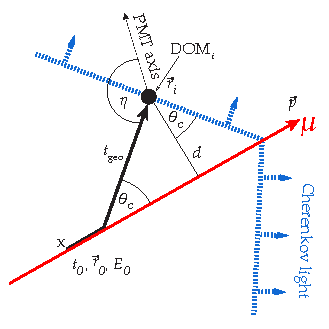
\includegraphics[width=0.6\textwidth]{ic/amanda_reco.pdf}
    \caption[Angular reconstruction in IceCube]{Parametrization for the angular muon reconstruction, describing the trajectory of a muon (red line) with energy $E_0$ that is in position $\vec{r_0}$ at time $t_0$, traveling towards direction $\vec{p}$. Cherenkov light from that muon is detected by a DOM at position $\vec{r_i}$ at distance $d$ to the trajectory with a light travel time $t_\text{geo}$. Adapted from~\cite{Ahrens2004}.}
    \labfig{ic_reco_cherenkov}
\end{figure}

To simplify matters, we assume that we are dealing with a muon with maximum allowed speed ($\beta=1$), traveling along a track of infinite length. Furthermore, we neglect stochastic photon losses, which are mainly caused by impurities within the Antarctic ice (see below). The set of parameters $\vec{a}$ needed to describe the physical situation in the detector is visualized in Fig.~\ref{fig:ic_reco_cherenkov}: $\vec{a}$ = ($t_0$, $E_0$, $\vec{r_0}$, $\vec{p}$). They describe the trajectory of a muon located at position $\vec{r_0}$ with energy $E_0$ at time $t_0$, and traveling in the direction $\vec{p}$.

So we are dealing with one time parameter, one energy parameter and positional parameters in 5 dimensions, where the vertex position $\vec{r}_0$ can be expressed in (x,y,z) and the muon direction $\vec{p}$ is usually described by two angles, zenith and azimuth\sidenote{The zenith angle is the angle to a line vertical to the Earth, centered on the detector surface and pointing `southwards' (away from the Earth). An azimuth angle of \SI{90}{\degree} describes a particle traveling from North (prime meridian pointing towards Greenwich) to South, while a particle with an azimuth angle of \SI{0}{\degree} travels along the 90th Meridian from East to West.}. In the context of IceCube muon reconstruction, this parameter set $\vec{a}$ is known as the `track hypothesis'.

Now, a DOM in the detector at position $\vec{r}_i$ at a distance $d$ to the track can be hit by Cherenkov photons emitted by the muon traveling along the track with the Cherenkov angle $\theta_\text{C}$, arriving at an angle $\eta$ with respect to the PMT axis. Without scattering, the photon reaches the $\text{DOM}_i$ at the geometrical time $t_\text{geo}$, which can be expressed as

\begin{equation}
    t_\text{geo} = t_0 + \frac{|\vec{p}\cdot(\vec{r_i}-\vec{r_0})|+d\cdot \tan{\theta_\text{C}}}{c_0},
\end{equation}

with $c_0$ the vacuum speed of light. As this does not take scattering into account, it is useful to define a relative time of arrival, the time residual $t_\text{res} = t_\text{hit} - t_\text{geo}$. This is the additional time introduced by scattering as opposed to a Cherenkov photon traveling directly from the muon to the DOM\@.

The scattering does primarily not loose light, but delays the photons. It is dominated by Mie scattering on impurities located within the ice. These impurities are thought to mainly comprise mineral dust, salt, acid droplet and soot by volcanic activity, all deposited by snow fall in the course of the last \num{1e5} years~\sidecite{Abbasi2022a}.

As the position of the DOM is known, $t_\text{res}$ is the most significant observable for each DOM,  We therefore simplify $x_i$ to $t_{\text{res},i}$ and express $\vec{a}$ as a function of the individual DOM parameters: $\vec{a}= (d_i,\eta_i,\ldots)$, where $\eta_i$ is the angle to the DOM PMT axis (see Fig.~\ref{fig:ic_reco_cherenkov}).


\subsection{First (single) Photoelectron Fit}
Matters can be simplified further. While the muon is traveling and emitting Cherenkov light, multiple photons can hit each DOM\@. One simplification is to only regard the first photon hitting an individual DOM, as it is usually less scattered than the average photon. If the reconstruction is using this simplification, it is called Single Photoelectron (SPE) fit. The likelihood function for this is\sidenote{As stated above, this already includes the reduction of $x_i$ to $t_{\text{res},i}$.}

\begin{equation}
    \mathcal{L}_\text{1st}(\vec{x}|\vec{a}) = \prod_i^\text{1st hits} p(t_{\text{res},i}|\vec{a}=d_i, \eta_i,\ldots),
\end{equation}

where the probability density function $p(t_{\text{res},i}|\vec{a})$ is obtained from simulations modeling the photon propagation through the Antarctic ice (this is necessary because the photon scatter needs to be accounted for). The simulation results are either stored in look-up tables or approximated by analytical functions~\cite{Ahrens2004}.

\subsection{Multi Photoelectron Fit}
A complication is that one expects the first photon in a DOM detecting multiple photons \textit{earlier} than a photon detected by a DOM only registering a single photon. This is because more photon hits mean that the DOM is closer to the event, and therefore receives a higher signal --- which means that the event is detected earlier.

This leads to the Multi Photoelectron (MPE) fit. Here, the single photon part of the likelihood is modified by the cumulative PDF (CDF), which is given time-integrating the photon arrival PDF from the $t_\text{res}$ to infinity:

\begin{equation}
    P(t_{\text{res},i}|\vec{a}) = \int^{\infty}_{t_{\text{res},i}}p(t|\vec{a})\,dt.
\end{equation}

Using this, the MPE likelihood is given as

\begin{equation}
    \mathcal{L}_\text{MPE} = \prod_i^\text{1st hits} p(t_{\text{res},i}|\vec{a}) \cdot N_i \cdot (1-P(t_{\text{res},i}|\vec{a}))^{N_i-1},
\end{equation}

where $N_i$ is the total number of photons recorded by $\text{DOM}_i$~\cite{Ahrens2004}. This is almost what is used by the angular reconstruction used for the alerts IceCube distributes\sidenote{See Section~\ref{ic_alerts}.}. The difference is the PDF used, which is described in the following Section~\ref{spline_mpe}.

\subsection{\texttt{SplineMPE} Reconstruction}\label{spline_mpe}
So far, nothing has been said about the photon arrival time PDF $p(t|\vec{a})$. The most straightforward approach is using a Gaussian distribution, which models the muon moving through the ice as plane wave of constant velocity. This can be enriched by assuming a more physically correct minimally ionizing muon track. When doing so, the PDF becomes a Gamma distribution of the form
\begin{equation}
    p(t_\text{res}) = \frac{\beta^\alpha t_\text{res}^{\alpha-1} e^{-\beta t_\text{res}}}{\Gamma(\alpha)},
\end{equation}
where $\alpha=\frac{d_\text{eff}}{\lambda}$, $\beta=\frac{1}{\tau} + \frac{c_m}{\lambda_\alpha}$. Here $\lambda$ is the scattering length, $\lambda_\alpha$ the absorption length, $c_m$ is the speed of light in a transparent medium and $\Gamma$ is the Gamma function. $d_\text{eff}$ is a modified version of the distance to the DOM $d$, that takes into account that the PMTs face downwards, and light from a track above a DOM needs to scatter around the DOM first (thus introducing an additional angle). The scattering and absorption lengths $\lambda$ and $\lambda_a$, as well as the unspecified parameter $\tau$ have been determined by Monte Carlo simulations~\sidecite{Abbasi2021a}.

\texttt{SplineMPE} uses a more sophisticated PDF, as the Gamma PDF above assumes an optically homogenous medium. This is not the case for Antarctic ice. For this reason, a fitted ice model derived from measurements with the Flasher Board\sidenote{See Section~\ref{DOM}.} is used.

The basic idea is to create a large lookup table of simulated minimally ionizing muon tracks of infinite length with many different positions and orientations, i.e.\ high-dimensional histograms. A comprehensive look-up table of these simulations would be too storage intensive (hundreds of \unit{\giga\byte}), as well as numerically problematic due to empty bins or interpolation artifacts. To mitigate this, the histograms are normalized and interpolated with multi-dimensional basis splines~\sidecite{Whitehorn2013}. These splines then represent the photon arrival PDF dependent on the track vertex and orientation in the detector. They are defined by knots of fixed positions, so the PDF becomes
\begin{equation}
    p(t_\text{res}) = \sum_{i=1}^{T-k-1} w_i B_{i,k}(t_\text{res},\vec{a}, \kappa).
\end{equation}

\begin{marginfigure}
    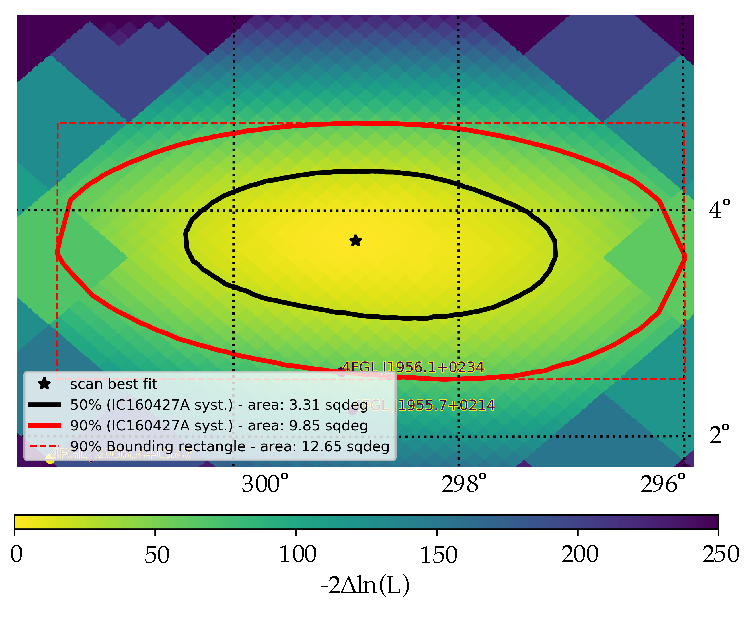
\includegraphics[width=1\textwidth]{ic/ic_millipede_IC221124A.pdf}
    \caption[\texttt{Millipede} reconstruction of \emph{IC221124A}]{\texttt{Millipede} reconstruction of \emph{IC221124A}.}
    \labfig{ic_millipede}
\end{marginfigure}

Here $T$ is the total number of knot positions, $B$ is the $i$-th basis spline of order $k$, $\vec{a}$ again describes the track, and $\kappa$ denotes the parameters of the ice model.

\subsection{\texttt{Millipede} Reconstruction}\label{millipede}

High-energy neutrino events that pass the realtime alert selection criteria (see Section~\ref{ic_alert_program}) are subjected to a more sophisticated algorithm, which uses the information from all the detected photons. This algorithm is dubbed \texttt{Millipede}. Due to its high demand of computational resources it is only run for selected events at the IceCube data center in Madison.

This reconstruction consists of a maximum likelihood scan covering the whole sky. To allow scanning, the sky is pixelated into grids of increasing resolution following the Hierarchical Equal Area isoLatitude Pixelation (\texttt{HEALPix}) scheme~\sidecite{Gorski2005}. Each pixel of a specific resolution covers the same area on the sky. For each scanned pixel, the muon direction is fixed to originate from that sky location.

For this fixed direction, the likelihood of the deposited energy resulting from the best fit and the neutrino interaction vertex in the detector are then computed. Pixels near the likelihood maximum are then subdivided with a finer \texttt{HEALPix} resolution. This procedure ultimately results in a likelihood map of the sky, with increasing granularity towards the global maximum~\sidecite{Abbasi2023}.

To compute the \SI{50}{\percent} and \SI{90}{\percent} confidence level uncertainty contours, Monte Carlo resimulations from the high-energy neutrino event \emph{IC160427A} are used. For this event, Pan-STARRS found a possible counterpart, \emph{PS16cgx}\sidenote{Spectroscopic follow up reveiled that this event was either a SN Ic, which would be compatible with neutrino production, or --- more likely --- a SN Ia, which would exclude it as a neutrino source.}~\sidecite{Kankare2019}.

In the resimulations, the systematic parameters of the Antarctic ice used to model photon propagation were varied. Additionally, the simulated direction and energies were varied, with cuts to ensure that the light deposition of the resimulations resembled the original event (\SI{\pm2}{\degree} in direction, \SI{\pm20}{\percent} in deposited charge).

Each resimulated event was fit with \texttt{Millipede}. The distribution of differences between the best-fit likelihood and the ground truth of the simulated event can then be employed to convert the change in log-likelihood over the map into a confidence level.

Due to the systematic uncertainties, Wilk's theorem does not apply here. To account for this fact, the contours derived for individual events (which make use of the theorem) are scaled up with correction values obtained from the resimulations of \emph{IC160427A}. Then, all pixels that satisfy $\log \mathcal{L}_\text{min}-\log \mathcal{L}_\text{pixel} = -11.3$ $(-32.1)$ form the \SI{50}{\percent} (\SI{90}{\percent}) error contours. Currently, these correction values are 22.2 and 64.2 for the \SI{50}{\percent} and \SI{90}{\percent} uncertainty contours~\sidecite{Gualda2021}. In Fig.~\ref{fig:ic_millipede} these contours are displayed for an example event. The black line shows the \SI{50}{\percent} uncertainty region, while the red line shows the \SI{90}{\percent} area.

However, resimulations of newer high-energy neutrino events have shown that the method of scaling up the errors with correction values obtained from resimulating \emph{IC160427A} does in some cases not faithfully capture the errors of those newer resimulations: They are sometimes under-, sometimes overestimated, depending on the topography of the event. For details on this, see~\cite{Gualda2021}.

\section{The Realtime Alert Program}\label{ic_alert_program}
Since 2016, IceCube hosts a realtime alert program, providing the astrophysical community with low-latency, high-quality astrophysical neutrino alerts~\cite{Aartsen2017a}. This program saw a major revision in 2019, when two new alert streams, named `Gold' and `Bronze', were created~\sidecite{Blaufuss2019}. As these are designed based on cuts reducing the IceCube background, one needs to understand the background events first.

\subsection{Background}\label{background}

When searching for the sources of astrophysical neutrinos, there are two major sources of background events in the IceCube detector. Both stem from secondary cosmic-ray particles from the Earth's atmosphere.

\begin{figure}[htb]
    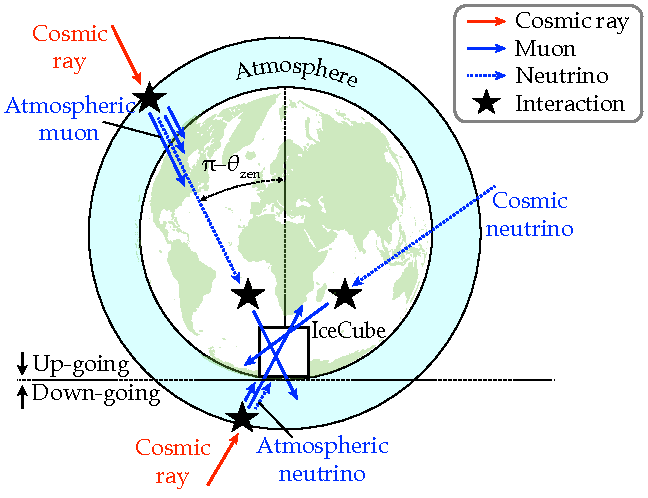
\includegraphics[width=0.8\textwidth]{ic/ic_background.pdf}
    \caption[Background events]{Background events in the detector. Cosmic rays hit the atmosphere around the globe and produce muons (solid blue arrows), as well as neutrinos (dashed blue arrows). When constraining to \textit{up-going} events from the northern hemisphere, the detector is shielded from atmospheric muons, but not atmospheric neutrinos, as these can traverse the Earth. Adapted from~\cite{Ahlers2018a}.}
    \labfig{ic_background}
\end{figure}

\begin{marginfigure}
    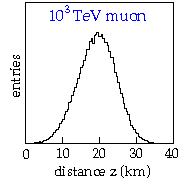
\includegraphics[width=0.8\textwidth]{ic/ic_muon_free_path.pdf}
    \caption[Muon free path in ice]{Free path length for \SI{1}{\peta\eV} muons in ice. The mean free path in ice is slightly longer than in rock. From~\cite{Chirkin2004}.}
    \labfig{ic_muon_free_path}
\end{marginfigure}

\begin{description}
    \item[Atmospheric Muons] are created by cosmic rays hitting the atmosphere. One can efficiently filter this background by restricting the analysis to \textit{up-going} muon tracks. These are tracks that come from the bottom of the detector, i.e.\ the northern hemisphere. Atmospheric muons stemming from cosmic-ray events in the northern hemisphere are filtered out by the Earth's core (see Fig.~\ref{fig:ic_background}), as the mean free path of muons within the Earth is much smaller~\sidecite{Chirkin2004} than the distance they have to cross (see Fig.~\ref{fig:ic_muon_free_path}). Note that due to light scattering within the ice, some down-going tracks can be misclassified as up-going~\sidecite{Ahlers2018a}.

          One complication here stems from the fact that the Earth starts to become opaque for neutrinos of higher energies. Studies interested in \si{\peta\eV} neutrinos therefore must deal with the fact that these get the more suppressed the longer their path through the Earth is. For example, a \SI{1}{\peta\eV} neutrino with a zenith angle of \SI{140}{\degree} is absorbed with \SI{90}{\percent} probability~\sidecite{Aartsen2017c}.

          \begin{figure}[htb]
              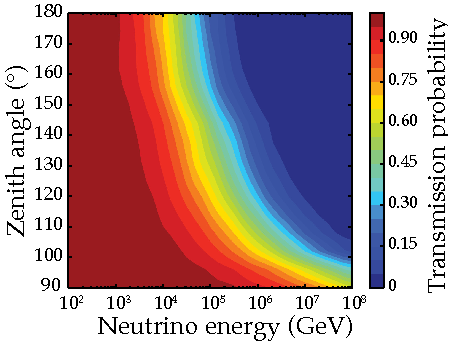
\includegraphics[width=0.5\textwidth]{ic/ic_absorption_earth.pdf}
              \caption[Neutrino absorption in the Earth]{Neutrino transmission probability through the Earth. The longer the distance traveled (higher zenith angles) and the higher the neutrino energy, the more likely is absorption. From~\cite{Aartsen2017c}.}
              \labfig{ic_absorption_earth}
          \end{figure}

    \item[Atmospheric Neutrinos] also stem from cosmic-ray induced air showers. These cannot be suppressed by directional cuts, creating an irreducible background: When atmospheric neutrinos cross the Earth and interact with the matter close to the detector, they can produce muons indistinguishable from muons created by `proper' cosmic neutrinos~\cite{Ahlers2018a}.

\end{description}

\subsection{Event Selection}\label{ic_event_selection}

Gold and Bronze alerts are drawn from three different selection schemes, originally designed to cater to different science goals. These are High Energy Starting Events (HESE)~\sidecite{Abbasi2021}, Extremely High Energy (EHE) events~\sidecite{Aartsen2016} and Gamma-Ray Follow Up (GFU) events~\sidecite{gfu2016}.

\begin{description}

    \item[HESE] are events that start \textit{within} the detector. This is guaranteed by using the outer regions of the detector as a veto region, in which (almost) no Cherenkov light must be detected~\cite{Aartsen2013}. The sizes of those regions can be seen in Fig.~\ref{fig:ic_hese_veto}. The majority of HESE events are cascade-type events and therefore not well suited for observational follow-up due to their poor angular reconstruction. Because of this drawback, additional cuts are applied: At least 6000 photoelectrons are required, and the reconstruction must favor a track interpretation of the event, and the reconstructed track length must be at least \SI{200}{\meter}~\cite{Abbasi2023}. Note that the selection criteria used in the Gold and Bronze HESE selection are slightly different than those in the original paper cited above.

    \item[EHE] aims at neutrino energies of \SIrange{0.5}{10}{\peta\eV}. To reject atmospheric background events, a two-dimensional cut depending on the reconstructed zenith angle and the log of detected photoelectrons is applied. Additionally, a $\chi^2$-based goodness-of-fit cut is applied to select track-like events with good reconstructions~\cite{Abbasi2023}.

          \begin{marginfigure}
              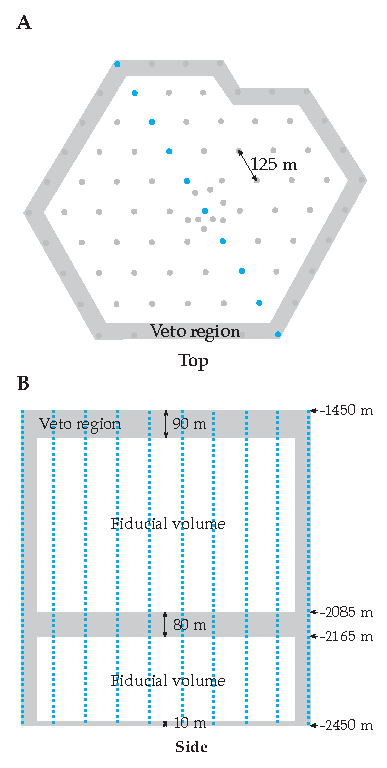
\includegraphics{ic/ic_HESE_veto.pdf}
              \caption[HESE veto regions]{High-energy starting events veto regions. The strings marked in blue in the top-down view at the top (A) show the location of the side view, displayed at the bottom (B). From~\cite{Aartsen2013}.}
              \labfig{ic_hese_veto}
          \end{marginfigure}

    \item[GFU] events are selected based on a boosted decision tree trained to identify \textit{through-going} (as opposed to `starting') track events with astrophysical origin. Energy cuts are applied: Northern hemisphere events are selected based on their reconstructed muon energies, while from the southern hemisphere are selected based on the total photoelectron charge deposited in the detector.
\end{description}

The cuts from all three event pools are gauged to achieve two different average values of signalness, which is a proxy for the probability that the event is of astrophysical origin~\cite{Abbasi2023}. It is defined as
\begin{definition}\label{signalness_def}
    $\text{Signalness}(E,\theta_\text{zen}) = \frac{N_\text{signal}(E,\theta_\text{zen})}{N_\text{signal}(E,\theta_\text{zen})+N_\text{background}(E,\theta_\text{zen})}$
\end{definition}
Here E is the reconstructed neutrino energy, and $N_\text{signal}(E,\theta_\text{zen})$ and $N_\text{background}(E,\theta_\text{zen})$ are the number of signal and background events at zenith angle $\theta_\text{zen}$ above energy $E$ as determined by simulations~\cite{Abbasi2023}.

The cuts on the individual event selections are tuned to ensure that \textit{Gold} alerts on average have a signalness $\langle \SI{50}{\percent} \rangle$, and \textit{Bronze} alerts have a signalness $\langle \SI{30}{\percent} \rangle$.

\subsection{Alert Distribution} \label{ic_alerts}
All events that pass a first stage of filtering are sent to the IceCube data center (see Section~\ref{data_acquisition}) via Iridium satellite to minimize latency. There, their signalness is computed. After this, they are globally distributed with the General Coordinates Network\sidenote{\url{https://gcn.nasa.gov/}} (GCN) in the form of GCN Notices.

Each notice contains the discovery time, a unique event number, the reconstructed direction in right ascension (RA) and declination (Dec) of the candidate neutrino computed by \texttt{SplineMPE}\sidenote{See Section~\ref{spline_mpe}.}, a statistical error for the direction, the reconstructed neutrino energy, the signalness and the false alarm rate~\cite{Blaufuss2019}.

\begin{marginfigure}
    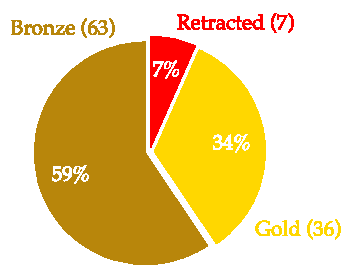
\includegraphics{ic/ic_he_alert_overview.pdf}
    \caption[IceCube alert overview]{High-energy neutrino alerts issued by IceCube since start of the new alert stream in June 2019.}
    \labfig{ic_he_alert_overview}
\end{marginfigure}

Those informations are later appended by \texttt{Millipede}, a computationally more demanding, but more sophisticated reconstruction (see Section~\ref{millipede}). The results of these reconstructions (i.e.\ the angular uncertainty) are typically distributed a few hours after the initial notice in the form of a GCN circular, and an updated GCN notice~\cite{Blaufuss2019}.

As of March 2023, a total of 106 events have been distributed in this format, with 7 later being retracted. Since the start of the Gold and Bronze alert stream in June 2019, this amounts to 2.2 non-retracted alerts per month\sidenote{This is quite close to the 2.5 alerts per month predicted in~\cite{Blaufuss2019}.} (0.8 Gold alerts, 1.4 Bronze alerts). For a full list of all high-energy neutrino alerts issued by IceCube, not only those since introduction of the Gold and Bronze format, see~\cite{Abbasi2023}.

If the event is most likely astrophysical and reasonably well pin-pointed, one can scan the sky localization with a telescope and look for potential sources of the neutrino. But where to obtain optical images from? The telescope used for this, the Zwicky Transient Facility, will be described in Chapter~\ref{ztf}.




\setchapterimage[7cm]{ztf/ztf_telescope.png}
\chapter{The Zwicky Transient Facility} \label{ztf}
\labch{ZTF}
The second instrument relevant for this thesis is the Zwicky Transient Facility (ZTF). It is named after the notorious Swiss-American astronomer Fritz Zwicky\sidenote{He first employed the Virial theorem to infer the existence of dark matter \cite{Zwicky1933}. Furthermore, together with Walter Baade, he posited the existence of supernovae and the creation of neutron stars in such events \cite{Baade1934}.}.

ZTF is a wide-field optical survey telescope. Its wide field means that its use case is to periodically scan the full sky, in contrast to getting pictures of specific objects. As its angular resolution is poor, ZTF is most sensitive to changes in brightness and therefore to the detection of transient events (short: \textit{transients}).\sidenote{Transient astrophysical events are observed as the time evolution of flux at different wavelengths from a small region on the sky.}

 ZTF is located at Mount Palomar in California, United States, at \SI{1700}{\m} above sea level, roughly \SI{130}{\km} southeast of Los Angeles. Its optical system, the \SI{1.2}{\m} (48 inch) Samuel Oschin telescope, follows a Schmidt design (see below\todo{Section}) and was inaugurated in 1948 \cite{Harrington1952}. At first light and for years to come, it was the largest Schmidt telescope in the world. Originally, the telescope exposed photographic plates, covering a field of view (FoV) of \SI{44}{\square\deg}. As such photographic plates have obvious drawbacks, and because technological progress made it possible, the Near-Earth Asteroid Tracking (NEAT) program \sidecite{Pravdo1999} replaced them with a charge-coupled device (CCD) camera in the early 2000s.\marginnote{See \url{https://sites.astro.caltech.edu/palomar/about/telescopes/oschin.html} for a historical overview.}

During the following years, the camera was updated several times\todo{twice? how often?}. The immediate predecessor of ZTF, the Palomar Transient Factory (PTF) \sidecite{Law2009}, began operation in 2009. Equipped with a 96 Megapixel camera, it already had many of the characteristics of ZTF: A fully automated survey, searching for optical transients with a CCD camera.

ZTF follows the concept of PTF, but is equipped with a larger and more sensitive camera. With \SI{47}{\square\deg}, the 600 Megapixel camera covers the full FoV of the P48. The main design metric for ZTF was \textit{volumetric survey speed}. This is the volume within which an object of given absolute magnitude can be detected in one exposure, divided by the total time for the exposure (observation plus overhead) \sidecite{Bellm2016}. The system saw first light in 2017, and started scientific operations in 2018 (the first survey data was taken on 2018-03-20). As of writing, ZTF is still operational.

There are two other telescopes located on Mount Palomar: The \SI{1.5}{\meter} (60 inch) P60 telescope houses the SED Machine (SEDM) \sidecite{Blagorodnova2018}, a fully robotic, low-resolution spectrograph used for automatic classification of transients. The largest facility on the mountain is the 200-inch (\SI{5.1}{\meter}) Hale Telescope, which is used for optical and infrared photometry as well as mid- and high-resolution spectroscopy of fainter sources. Together, these telescopes form a natural hierarchy: ZTF is the discovery engine for optical transients. Promising sources are then classified with SEDM. If a source warrants it, deeper photometry and better resolved spectroscopy can then be obtained with the P200. All three telescopes are shown in Fig. \ref{fig:palomar_overview}.

\begin{figure*}[]
    \includegraphics{ztf/palomar_overview.pdf}
    \caption[View of Mt. Palomar]{View of Mt. Palomar with the three telescopes highlighted in the text. Image credit: Caltech, annotations by the author.}
    \labfig{palomar_overview}
\end{figure*}

\section{Telescope Design}
A \textit{Schmidt telescope} like ZTF is by design dedicated to taking images, contrary to earlier designs allowing to observe through an eyepiece \sidecite{Schmidt1938}. For this reason, it is also referred to as a \textit{Schmidt camera}. The design goal was a wide FoV. This made it the ideal instrument for sky surveys, where a large FoV maximizes the on-sky area that can be monitored. A Schmidt telescope combines a spherical mirror at the end of the telescope tube with an aspherical correcting lens (Schmidt plate) at the tube's entrance. The use of a spherical mirror combined with the correcting lens gets rid of comatic aberration\todo{zusatz oder das ist nur blabla}.

\begin{figure}[]
    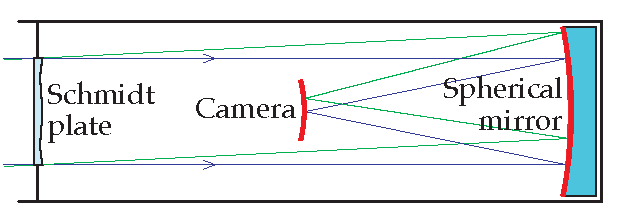
\includegraphics[width=1\textwidth]{ztf/schmidt2.pdf}
    \caption[Schmidt telescope schematic]{Schmidt telescope schematic. Light enters from the left, passes the Schmidt plate (an aspherical correcting lens), gets reflected by a spherical mirror at the end onto a photographic plate or camera halfway down the tube. Figure adapted from \url{https://commons.wikimedia.org/wiki/File:Schmidt-Teleskop.svg}.}
    \labfig{schmidt_telescope}
\end{figure}

Until the end of the 20th century, around ten Schmidt telescopes have been built, most of them to conduct sky surveys \sidecite{Cannon1995}. At least two of them were space telescopes: ESA's astrometry mission \textit{HIPPARCOS} \sidecite{ESA1997} (1989--1993) and the NASA explanet mission \textit{Kepler} \sidecite{Koch2010} (2009--2018). In both cases, the mission entailed monitoring of large areas of the sky; prime territory for Schmidt telescopes.

\begin{figure}[]
    \includegraphics[width=1\textwidth]{ztf/ztf_fov.pdf}
    \caption[ZTF Field of View]{ZTF field of view (highlighted in red) in comparison to other sky survey telescopes, including the future Rubin observatory (LSST) \cite{Ivezic2019}. Note also the 6.5-fold increase with respect to ZTF's predecessor, PTF/iPTF. From \cite{Laher2018}, highlighting by the author.}
    \labfig{ztf_fov}
\end{figure}



\section{Camera}
\begin{marginfigure}
    \includegraphics{ztf/ztf_camera_detail_highres.jpg}
    \caption[ZTF camera cutaway]{The ZTF camera in detail. From \cite{Dekany2020}.}
    \labfig{ztf_camera_detail}
\end{marginfigure}
The ZTF camera is a CCD design, consisting of 16 individual CCDs by commercial manufacturer e2v (now Teledyne, \textit{Science CCD231-C6}), each having 6144x6160 pixels, resulting in a total camera resolution of $\sim 600 \,\textrm{Megapixel}$ \sidecite{Dekany2016}. As one can see in Fig. \ref{fig:ztf_camera}, the array of 16 CCDs is slightly bent. This is necessitated by the Schmidt design, where the camera needs to be spherical, matching the spherical mirror. As individual CCDs are flat, each of the 16 sensors is is installed slightly tilted, tracing the overall curvature. To get rid of residual deviations from the global curvature, in front of each sensor a field flattener lens is mounted \sidecite{Bellm2019}.

\begin{marginfigure}
    \includegraphics{ztf/ccd_buckets.pdf}
    \caption[CCD operational principle]{CCD operational principle, explained with buckets measuring precipitation. From \cite{Janesick1987}.}
    \labfig{ccd_buckets}
\end{marginfigure}

\subsection{CCDs}
CCDs are silicon-based light sensors. They consist of arrays of coupled metal-oxide semiconductor (MOS) capacitors. Each one these is able to store the charge created by incident photons; spatial resolution is achieved by having one capacitor per pixel of the sensor array. The array is then exposed to light for a specified amount of time (exposure time). During the exposure, incident photons create a charge proportional to the amount of light hitting each capacitor via the photo-electric effect. This charge is accumulated in each capacitor until the exposure is finished. To read out the CCD, the charges need to be moved to neighboring capacitors. When the MOS capacitors are tightly placed, one can move the charges from one capacitor to the next by changing the voltages on the capacitor's gates.

In Fig. \ref{fig:ccd_buckets} the principle of a CCD is explained with little buckets collecting rain water. Each bucket symbolizes one capacitor or one pixel of the sensor array respectively. After the rain has stopped (the exposure is finished), each bucket naturally contains an amount of water proportional to the amount of water that rained down over it. Now the amount of water in each bucket (the charge deposited by incident light in each capacitor) needs to be measured.

To do this, the buckets in each row are moved one position to the left with horicontal conveyor belts. Each bucket at the left end of the horicontal conveyor belt is then emptied into the bucket on the single vertical conveyor belt. The buckets of this vertical belt are then one by one drained into the meausuring bucket on the bottom left. After all buckets on the vertical belt are emptied, the process starts anew, until all buckets are empty. As one can see, the time this process takes is quadratic to the amount of buckets (or pixels) \sidecite{Janesick1987}. To speed up the process, one can subdivide the sensor area into smaller sections, which are read out in parallel.

Each CCD pixel actually consists of three electrodes, which can be seen in Fig. \ref{fig:ccd_transport}. The transport of charge within the CCD is realized by subsequently applying a higher voltage to different electrodes, moving the charge step-wise. 

\begin{figure}[htb]
    \includegraphics[width=0.7\textwidth]{ztf/ccd_transport.pdf}
    \caption[Charge transport in a CCD]{Charge transport in a CCD. High voltage electrodes are shown filled, while low voltage electrodes are empty. By stepping through different combinations of electrodes, the electric potential changes, and the charge moves.}
    \labfig{ccd_transport}
\end{figure}

The typical exposure for the ZTF camera is \SI{30}{\second}, while the readout time (transferring and measuring the charge in each capacitor) is \SI{8.2}{\second}. Readout and digitization is done in parallel for four quadrants, each containing 4 CCDs. The four readout devices for the quadrants are \textit{Archon} CCD controllers by Semiconductor Technology Associates (STA), operated at \SI{1}{\mega\Hz}. Each of these operates 16 simultaneous readout channels, four for each CCD. In total, the camera is simultaneously read out in 64 independent regions to speed up the process.

Four additional smaller CCDs (2k x 2k pixels) are used as guidance, tip, tilt and focus sensors, with one additional Archon controller to read them out \sidecite{Dekany2020}. To reduce the thermal noise of the camera, it was placed on a cold plate, which is cooled by a cryocooler to \SI{160}{\kelvin} \cite{Dekany2016}.

\begin{figure}[htb]
    \includegraphics[width=1\textwidth]{ztf/ztf_camera.pdf}
    \caption[ZTF camera]{The ZTF camera. One can see the CCDs sandwiched between the filter on the front and the cryostat on the back. From \cite{Bellm2019}.}
    \labfig{ztf_camera}
\end{figure}

\section{Optical System}

\subsection{Filters and shutter}
As the CCDs of the camera cannot ``see'' color, different filters must be placed in front of the camera. Color information can then be obtained by imaging the object in question with a least two filters. ZTF employs three different filters: A \textit{g}-band filter with a median wavelength of \SI{472}{\nano \meter} (corresponding to blue light), an \textit{r}-band filter (median wavelength: \SI{634}{\nano \meter}, red light) and an \textit{i}-band filter (\SI{789}{\nano \meter}, near-infrared). These filters can be exchanged with a robotic arm, securely stowing the replaced filter and magnetically attaching the new one \cite{Dekany2020}; a process taking \SI{110}{\second} \cite{Bellm2019}. 

The main decision goal for the filter selection was to maximize the signal-to-noise ratio by avoiding major sky emission lines at Mt. Palomar while avoiding excessive costs. ZTF does not exactly match the filters of potential calibrators, e.g. the Sloan Digital Sky Survey (SDSS) \sidecite{York2000}, PanSTARRS (PS1) \sidecite{Kaiser2002} or \textit{Gaia} \sidecite{Prusti2016}. This was justified with the overall different telescope design of ZTF \cite{Bellm2019}.

\begin{marginfigure}
    \includegraphics{ztf/ztf_throughput.pdf}
    \caption[ZTF filter transmission]{ZTF filter transmission for the three different bands (\textit{g}-band: blue, \textit{r}-band: orange, \textit{i}-band: red). The green and gray datapoints show the CCD quantum efficiency measurements (single and double-layer reflective coating). From \cite{Bellm2019}.}
    \labfig{ztf_transmission}
\end{marginfigure}

The transmission of each filter and the CCD quantum efficiency curve can be seen in Fig. \ref{fig:ztf_transmission}. As one can see, the quantum efficiency starts to decrease within the \textit{r}-band towards higher wavelengths, rendering the \textit{i}-band the least sensitive of the three filters. The $5\sigma$ median sensitivity for a 30s exposure reflects that fact. It is 20.8 (21.1) mag in the \textit{g}-band, 20.6 (20.9) mag in the \textit{r}-band and 19.9 (20.2) mag in the \textit{i}-band; with values for optimal conditions (new moon) in brackets. The resulting median image quality is 2.1'' (\textit{g}-band), 2.0'' (\textit{r}-band) and 2.1'' full width at half maximum (FWHM) of the point spread function (PSF, see Section \ref{psfphot} below) \cite{Bellm2019}.

To decrease light obstruction, the ZTF shutter was newly developed and is mounted in front of the aperture, outside of the telescope tube. It was developed by Deutsches Elektronen-Synchrotron (DESY) in cooperation with industry partner Bonn-Shutter and allows to open and close in \SI{290}{\milli \second} \cite{Dekany2020}.

\subsection{ZTF grid} \label{ztf_grid}
One exposure during regular operations -- in contrast to e.g. deep target of opportunity (ToO) images -- lasts \SI{30}{\second}. There is an additional \SI{\sim 15}{\second} overhead for readout and slewing the telescope. Also some additional time is needed to exchange the filters. Therefore, a typical night lasting \SI{8.67}{\hour} \sidecite{Masci2019} results in roughly 700 exposures. In total, these amount to a sky area of over \SI{32500}{\square\deg}, allowing to cover the full visible sky at Mount Palomar \SI{15}{\degree} above the horizon at least once.

\begin{marginfigure}
    \includegraphics{ztf/ztf_g_band_grid3.pdf}
    \caption[ZTF field visits]{Number of ZTF \textit{g}-band field visits during the first week of May 2020. The primary grid fully tiles the sky accessible at Mount Palomar.}
    \labfig{ztf_g_field_visits}
\end{marginfigure}

To enable robotic control, ZTF operates on a fixed primary on-sky grid of so-called \textit{fields}. Each field corresponds to a fixed sky location with an area of \SI{47}{\square\deg}; the telescope exclusively points to those fields. With such a system, some parts of the sky will always fall into the chip gaps (the parts of the FoV that fall between the 16 CCDs). To mitigate that, there exists a \textit{secondary grid} that is diagonally offset from the primary grid, with \SI{0.29}{\degree} average overlap in right ascension, and \SI{0.26}{\degree} in declination \sidecite{Bellm2019a}. Fig. \ref{fig:ztf_g_field_visits} shows the primary grid and the number of visits per field in the \textit{g}-band during the first week of May 2020.

\section{Calibration and Image Processing}
The ZTF image processing can be divided into two parts: The science exposures are taken at Mount Palomar, while calibration, extraction of transients and archival storage happens at the Infrared Processing and Analysis Center (IPAC)\sidenote{\url{https://www.ipac.caltech.edu}} situated on the campus of the California Institute of Technology (Caltech). IPAC ultimately hosts the ZTF images as part of IRSA\sidenote{\url{https://irsa.ipac.caltech.edu}}, the Infrared Science Archive.

\begin{marginfigure}
    \includegraphics{ztf/ztf_calibration_flow.pdf}
    \caption[ZTF realtime flowchart]{Flowchart of the ZTF calibration, starting with the raw images on the top and ending with the final science products on the bottom. Adapted from \cite{Laher2018}.}
    \labfig{ztf_calibration_flow}
\end{marginfigure}

The full calibration and image processing pipeline is shown in Fig. \ref{fig:ztf_calibration_flow}. First come the different calibration steps: overscan and bias correction, flat fielding, as well as astrometric and photometric calibration. This is followed by creating the difference images and finally extracting the sources. I will briefly explain the different steps in the next sections.

\subsection{On-site processing and datalink}\label{ztf_data_link}

Each image taken on site (calibration and science exposures alike) is stored as FITS file and subsequently compressed loslessly. The compressed images on average use \SI{5}{\bit} per pixel, so the full image is roughly \SI{380}{\mega\byte} large. These images are immediately sent to IPAC with the High Performance Wireless Research \& Educational Network (HPWREN)\sidenote{\url{https://hpwren.ucsd.edu/}}, a microwave-based data network, linking Palomar Observatory with the IPAC post-processing site. Each transfer typically takes \SI{20}{\second}, keeping up with the pace of ZTF observations \cite{Dekany2020}.

\subsection{Overscan correction}
As the temperature of the CCDs changes with time, each image is subject to a time-dependent global offset induced by thermal noise. To correct for this, an \textit{overscan} region is used. In the case of the ZTF CCDs, this region does not correspond to physical pixels, but is created during CCD readout. If one reads out more clock cycles then pixels are available, the charge that has gathered during science readout can be accessed. For ZTF, this is done for an additional 24 cycles, corresponding to 24 overscan pixels for each sensor row. After this, the median of these 24 pixels is taken and the full overscan column is fitted with a quadratic function. For each and every image taken by the camera, the bias described by this quadratic function is calculated and subtracted from the image \cite{Masci2019a}.

\subsection{Bias correction}
The CCD pixels also have different noise levels, meaning in the absence of external photoelectrons they still generate a signal, which is different from pixel to pixel -- i.e. their zero point differs. Luckily, this variation has a higher degree of time-stability \sidecite{Howell2006}. To correct it, at the beginning of each night at least 10 so-called \textit{bias} images are taken and overscan corrected. These images are zero-second exposures which are then stacked. After this, the truncated mean of each pixel is calculated, constituting the final bias image for the night (and filter). This bias image is subtracted from each science exposure using the respective filter taken during the night \cite{Masci2019a}.

\subsection{Flat fielding}
The pixels in the CCDs do not only differ in zero point, they also have slightly different gain or quantum efficiency. This means, their response to light is not uniform. To account for this, the calibration needs a structureless, uniformly bright light source against which the individual pixel response can be measured \cite{Howell2006}. In the case of ZTF, this is achieved by using a flat field illuminator consisting of a round screen illuminated by eight identical boards with LEDs, each board housing $4\times15=60$ LEDs of 15 different colors, covering the full wavelength region of ZTF \cite{Dekany2020}.
\begin{marginfigure}
    \includegraphics{ztf/ztf_flatfield_illuminator.png}
    \caption[ZTF flat field illuminator]{The ZTF flat field illuminator. From \cite{Dekany2020}.}
    \labfig{ztf_flatfield_illuminator}
\end{marginfigure}
Each afternoon, before science operations begin, at least 20 images per filter are taken of the flat field illuminator. These are then overscan corrected, the bias image is subtracted, and the pixel values are normalized to a truncated global mean of 1 over the image (to allow for later division). After this individual treatment, all flat field images per filter are stacked to a truncated mean per pixel and outlier rejection is applied to isolate additional noisy pixels. All science images taken during the night are divided by this flat field image \cite{Masci2019a}.

\subsection{Astrometric calibration}
Astrometric calibration is the mapping of image pixel coordinates to an on-sky coordinate system. For ZTF, this is performed with stars contained in the \textit{Gaia} Data Release 1 (\textit{Gaia} DR1, \sidecite{Brown2016}). As it is a mission designated to high-precision astrometry, \textit{Gaia} is the ideal reference for this task. Prior to cuts, the DR1 contains over 1 Billion sources. From these, sources are selected that are neither too faint, nor run risk of saturating the detector ($12 \leq G \leq 18$ mag). The astrometric solution is derived using the \texttt{SCAMP} \sidecite{Bertin2006} package \sidecite{Masci2019}. For this, stars are extracted with \texttt{SExtractor} \sidecite{Bertin1996} and matched to the \textit{Gaia} stars. The pointing, rotation and polynomial distortion needed to match the stars constitutes the astrometric solution.

\subsection{PSF photometry} \label{psfphot}
After astrometric calibration, sources in the image need to be extracted to perform photometric calibration (to compare star brightnesses to reference measurements, one first needs stars...). To do so, point spread function (PSF) photometry is employed. Each telescope has a finite aperture, therefore suffering from diffraction. Additionally, earth's atmosphere is constantly and turbulently changing, with different atmospheric layers having different refractive indices, depending on their temperature. This smears out the light from the original point source, an effect known as \textit{seeing} (see Fig. \ref{fig:seeing}).

\begin{figure}[h!]
    \includegraphics{ztf/seeing.pdf}
    \caption[Seeing]{\textit{Seeing}: Atmospheric distortions cause time-dependent distortions in the wavefronts, which average out during the exposure and form a Gaussian seeing disk on the sensor (bottom right image). Adapted from \cite{Chromey2016}.}
    \labfig{seeing}
\end{figure}

The PSF is describing the way an ideal point source is smeared out spatially after being subjected to atmospheric and optical effects in the telescope, and seeing is the FWHM of the PSF. The algorithm used to reconstruct the PSF of a ZTF exposure is \texttt{DAOphot} \sidecite{Stetson1987}. It fits an analytic Gaussian profile to all point sources within an image. After subtracting this profile, it is iteratively updated with the residuals after subtraction. The background estimate needed for this procedure is extracted from the peak brightness value of a histogram of evenly distributed pixels within the image \cite{Stetson1987}.

\subsection{Photometric calibration and magnitudes} \label{magnitudes}
\marginnote{Of course, PS1 needs to be calibrated in itself. That is done in two steps: A self-consistent relative calibration is created with \texttt{Ubercal} \cite{Schlafly2012}. This relative calibration is in turn anchored to precisely measured \textit{Calspec} standard stars. For details, see \cite{Magnier2020}.}
Not only the source positions in the images need to be calibrated (astrometry), but their brightness as well (photometry). To simplify matters, ZTF is photometrically calibrated against a reference survey, namely PS1. To do this, a catalog of useful calibrator stars from the PS1 survey has been curated. These stars are required to fulfill some basic quality criteria: They should be stable over multiple PS1 survey epochs in all PS1 filters excluding the \textit{y}-band (\textit{g}, \textit{r}, \textit{i}, \textit{z}) and should be fairly bright, but not so bright that they saturate the ZTF sensors. Furthermore, they are required to be fairly isolated to avoid blending with neighboring objects and need to have a high probability of being in fact stars (as opposed to galaxies) \cite{Masci2019a}.

The brightness of both ZTF and PS1 are measured in magnitudes. Magnitudes are somewhat counterintuitive, as a higher value corresponds to a fainter source.\sidenote{This can be traced back over 2000 years to Greek/Roman astronomers Hipparchus and Ptolemy \cite{Krisciunas2001}. These classified the brightest stars to be of ``first order'' or ``first magnitude'', with subsequently dimmer stars assigned lower magnitudes until the dimmest stars visible to the naked eye were of ``sixth magnitude''. The system stuck and was put on firm footing by Norman Pogson in 1856. He defined a star being 5 magnitudes brighter than another one to be 100 times brighter \cite{Jones1968}.} The following definition holds:

\begin{definition}
\labdef{magnitude}
A star one magnitude brighter than another star is $\sqrt[5]{100} \approx 2.512$ times brighter
\end{definition}
If one uses flux density (power per unit area) on earth as a measure of brightness, it follows from Def. \ref{def:magnitude} that the difference between two objects with magnitudes $m_1$ and $m_2$ and respective flux densities $f_1$ and $f_2$ is:
\begin{equation}
m_1 - m_2 = -2.5 \log_{10}{\frac{f_1}{f_2}}
\end{equation}
Now we have a \textit{relative} definition of an source's magnitude, but we need an absolute one. In other words, one needs to know what constitutes a magnitude of 0 (the zero point of the magnitude scale). ZTF uses AB magnitudes \sidecite{Oke1983}, which are defined via the spectral flux density $f_\nu$ [\unit{\W\per\m\per\Hz}]. In this sytem, the magnitude is a logarithm of the spectral flux density: 

\begin{definition}
\labdef{abmag_density}
$m_{\text{AB}}(\nu) = -2.5 \log_{10}{(f_\nu/\SI{3631}{\jansky})}$
\end{definition}

As one can see, a source with constant spectral flux density $f_{\nu,0} = \SI{3631e-23}{\W\per\cm\per\Hz} = \SI{3631}{\jansky}$ corresponds to a magnitude of 0.\sidenote{The value of $f_\nu,0$ is not entirely random: The traditional zero point was the star Vega. Vega's magnitude in the AB system as defined above, integrated over the \textit{V}-band, is 0.03, close to the traditional 0. The AB system has the advantage of not relying on a physical source.} Now, telescopes like ZTF and PS1 use bandpass filters, so the spectral flux density is integrated over the filter wavelengths. Therefore, the magnitude definition changes to \sidecite{Tonry2012}:

\begin{definition}
\labdef{abmag}
$m = -2.5 \log_{10}{\frac{\int{f_\nu(h \nu)^{-1}A(\nu)\,d\nu}}{\int{\SI{3631}{\jansky}(h \nu)^{-1}A(\nu)\,d\nu }}}$
\end{definition}
Here, $h$ is Planck's constant and $A(\nu)$ is the capture cross section (i.e. the chance of an incoming photon to produce an electron in the detector\sidenote{More general, $A(\nu)$ is $A(\nu,\theta,t)$, also depending on the angle of the incoming photon and therefore the atmospheric column along the line of sight, as well as time.}). ZTF does not use a precisely modeled response function $A(\nu)$, but relies on PS1. To first order, ZTF magnitudes are tied to the PS1 system via their zero point:

\begin{equation}
m_\text{cal} = m_\text{instr} + \text{ZP}
\end{equation}

To do this, all extracted sources are spatially matched to the PS1 calibrator catalog. After creating a one-to-one relation between ZTF stars and PS calibrator stars, one could to first order calculate $m_\text{cal}$.

But there is a potential complication: The ZTF and PS1 filters are fairly similar, but not exactly so. This means that a celestial object that does not have a constant spectrum (i.e. almost all of them) will have slightly different brightness values when measured with the ZTF and the corresponding PS1 filter. To account for this, a linear, filter-dependent \textit{color correction} $c_f$ needs to be applied:

\begin{equation}
m_\text{cal} = m_\text{instr} + \text{ZP}_f + c_f \times \text{PS1}_\text{clr}
\end{equation}
where $\text{PS1}_\text{clr}$ is filter dependent ($g_\text{PS1}-r_\text{PS1}$ for the ZTF \textit{g}/\textit{r}-band, and $r_\text{PS1}-i_\text{PS1}$ for the \textit{i}-band).

In the photometric calibration step, $\text{ZP}_f$ and $c_f$ are chosen to globally minimize $\Delta m_f = \text{ZP}_f + c_f \times \text{PS1}_\text{clr}$ for all calibrator stars in the respective image \cite{Masci2019a}.

\subsection{Image subtraction} \label{ztf_image_subtraction}
Because ZTF is a survey telescope deeply rooted in time-domain astronomy, many of the science goals concern observing sources that are \textit{new} or \textit{changing}. To do so, one needs to detect changes in the nightly observations with regard to \textit{reference images}. From all new images those reference images are subtracted (see Fig. \ref{fig:img_subtraction}). All remaining detections constitute temporal evolution with respect to the epoch of reference image creation. All reference images in ZTF are stacked images of 15--40 individual high-quality images, most of them created early after the start of telescope operations. Quality criteria for the individual images comprise good seeing, low errors on the astrometric and photometric calibrations, as well as background levels falling into filter-specific ranges \cite{Masci2019}.

\texttt{SWarp} \sidecite{Bertin2010} is used to interpolate and resample the reference image onto the science image, while subsequent subtraction and PSF photometry (see Section \ref{psfphot}) is performed with the \texttt{ZOGY} algorithm \sidecite{Zackay2016}.

\begin{figure}[h!]
    \includegraphics{ztf/ztf_imsub.png}
    \caption[ZTF image subtraction]{ZTF image subtraction. The new science image is on the left; in the middle is reference image, which is subtracted. This results in a \textit{difference image}, seen on the right. From \cite{Mahabal2019}.}
    \labfig{img_subtraction}
\end{figure}

\subsection{Alert packages} \label{ztf_alerts}
\begin{marginfigure}
    \includegraphics{ztf/ztf_bogus.png}
    \caption[ZTF subtraction artifact]{ZTF subtraction artifact, resulting in a bogus transient. From \cite{Mahabal2019}.}
    \labfig{ztf_bogus}
\end{marginfigure}

The last step in the imaging pipeline is alerting an array of upstream transient alert brokers. The information on new transients or updates on existing ones therefore need to be packaged into a convenient format. All positive detections after image subtraction with a signal-to-noise greater than 5 are subjected to \texttt{RealBogus}. This is a machine learning (ML) algorithm trained to discriminate between ``real'' events (most likely astrophysical) and ``bogus'' events (e.g. subtraction artifacts, see Fig. \ref{fig:ztf_bogus}) \sidecite{Mahabal2019}. This algorithm creates a \texttt{rbscore}, ranking the probability of the detection of being real.

Another ML algorithm has been employed to assign all PS1 sources a \texttt{sgscore}, separating between stars and galaxies based on their morphology and flux in all PS1 bands \sidecite{Tachibana2018}. Both \texttt{rbscore} and \texttt{sgscore}, as well as cutouts of the science, reference and difference images are packed together and shipped as \textit{alert package}. These alerts also include the distances to the three nearest PS1 sources, the closest \textit{Gaia} source, up to 30 days of previous detections if these exist, and some quality metrics like the limiting magnitude. The file format for distribution is Apache Avro\sidenote{\url{https://avro.apache.org}}, and the method of distribution is an Apache Kafka\sidenote{\url{https://kafka.apache.org}} stream \sidecite{Patterson2018}.

\section{Surveys and Cadence}
ZTF is supporting three main survey programs: First, there is the NSF Mid-Scale Innovations Program (MSIP) survey, which is allocated \SI{40}{\percent} of telescope time. The MSIP survey is subdivided into the Northern Sky Survey, using a large fraction (\SI{85}{\percent}) of MSIP time. This survey covers the entire \SI{23675}{\square\deg} of the northern sky \SI{7}{\degree} above the galactic plane. As long as a field (see Section \ref{ztf_grid}) is accessible, it is observed once in the \textit{g}- and once in the \textit{r}-band every 3 nights, with both images separated by at least 30 minutes to reject transients and moving (i.e. solar system) objects. The rest of the northern sky ($|b|\leq \SI{7}{\degree}$, with a footprint of \SI{2800}{\square\deg}) is visited twice per night, with the same observational parameters as the Northern Sky Survey \cite{Bellm2019a}.

Another \SI{40}{\percent} are allocated to the partners of the ZTF collaboration. During the first year of ZTF operation, this allocation was dedicated to the Extragalactic High Cadence Survey, the \textit{i}-band Survey, to ToO observations like the Neutrino Follow-up Program (see Chapter \ref{fupipeline}), to the Twilight Survey, the High-cadence Plane Survey and the Asteroid Rotation Period Survey \cite{Bellm2019a}.

The last \SI{20}{\percent} are private Caltech time, with surveys selected each semester by the Caltech Time Allocation Committee \cite{Bellm2019a}. A prominent example is the observational campaign to follow up 
LIGO-Virgo (LV) \sidecite{Aasi2015,Acernese2014} gravitational wave (GW) localizations during the 3rd observational run (O3) \sidecite{Kasliwal2020}.


\setchapterimage[7cm]{fu/heading3.png}
\chapter{The ZTF Follow-Up Pipeline} \label{fupipeline}
\labch{fupipeline}
After introducing the IceCube detector (see Chapter \ref{ic}) and the Zwicky Transient Facility (see Chapter \ref{ztf}), we now have all the ingredients to introduce the ZTF high-energy neutrino follow-up pipeline.

IceCube sends out \num{\sim2.2} astrophysical high-energy neutrino alerts on average per month\sidenote{See Section \ref{ic_alerts}}. Due to its large FoV and fully robotic operation, ZTF is the ideal follow-up instrument for these alerts. It allows to cover the typically reported IceCube localization regions with only one pointing of the telescope.

The follow-up procedure can be outlined as follows: An \textit{IceCube alert} is received. If the alert meets our \textit{alert quality criteria}, we do an \textit{observability check}. If the sky region is accessible to ZTF, we \textit{observe}. After observations, we \textit{filter} candidates with \texttt{nuztf} based on \texttt{AMPEL} \sidecite{Nordin2019}, followed by visual inspection. Lastly, we acquire forced photometry and -- if needed -- trigger \textit{additional follow-up}.

\section{Alert Cuts}\label{alert_cuts}
As we only have limited telescope time, we apply quality cuts on the high-energy neutrino alerts received via GCN Notices. As outlined in Section \ref{ic_event_selection}, there are two alert streams: \textit{Gold alerts} with an average purity of \SI{50}{\percent} (\SI{36}{\percent} of all non-retracted alerts), and \textit{bronze alerts} with an average purity of \SI{30}{\percent} (\SI{64}{\percent}).

In general, we only follow up if the reported bounding rectangle comprising the \SI{90}{\percent} uncertainty region\sidenote{See Section \ref{millipede}} covers less than \SI{40}{\square\deg}. All gold alerts making this cut qualify for follow up. There is a more stringent cut on the uncertainty areas of bronze alerts, requiring these are $<\SI{10}{\square\deg}$. To avoid contamination by foreground stars, we implement a cut on galactic latitude of $|b|>\SI{10}{\degree}$.

\section{Observation Planning with \texttt{planobs}}\label{planobs}
If an alert makes these cuts, one needs to check if observations with ZTF are feasible. To reduce the potential for errors, this is done with assistance by the \texttt{planobs} \sidecite{Reusch2023} tool, developed and maintained by the author to automate the task as much as possible.

\texttt{planobs} is written in Python, and is deployed on a virtual private server. The backend runs on \texttt{Flask}\sidenote{\url{https://flask.palletsprojects.com}} behind a \texttt{nginx}\sidenote{\url{https://nginx.com}} reverse proxy exposed to the internet. The \texttt{nginx} endpoint serves a Slack\sidenote{\url{https://slack.com/}} bot integrated into the DESY multimessenger group chat for ease of use. It can also be run locally.

The tool is designed to be used with a simple command-line-style interface in the Slack chat. For example, issuing
\begin{lstlisting}[language=bash,style=kaolstplain]
Plan IC221223A -multiday
\end{lstlisting}
in the \texttt{plan\_observations} Slack channel will create an observation plan for IceCube high-energy neutrino IC220501A, spanning multiple days.

To obtain the positional and error information on the neutrino in question from the respective GCN Circular, \texttt{planobs} is searching for the GCN on an experimental server\sidenote{\url{https://heasarc.gsfc.nasa.gov/wsgi-scripts/tach/gcn_v2/tach.wsgi}}. As circulars are written by humans, it fuzzily parses them to extract the relevant information. After this, observability at Mt. Palomar is calculated, defaulting to the current time (optionally, a desired observation time can be requested). 

\begin{figure}[h!]
    \includegraphics{fu/planobs_airmass.pdf}
    \caption[Observation plan]{Observation plot created by \texttt{planobs} for the follow-up of IceCube neutrino IC221223A. The altitude and airmass of the alert region at Mt. Palomar are shown in blue. The red and green shaded regions are proposed observation windows in the \textit{r}- and \textit{r}-band. The red arrows show the airmass limit of 2.0, and the moon is displayed as yellow dotted curve. The gray shaded region marks night-time at the telescope site. All information automatically extracted from the GCN Circular are shown on top.}
    \labfig{planobs}
\end{figure}

An example observability plot is shown in Fig. \ref{fig:planobs}. The blue curve shows the altitude of the neutrino sky region above Mt. Palomar, and the red and green shaded regions mark the two proposed observation windows in the \textit{r}- and the \textit{g}-band.

Additionally, for each field of the primary and secondary grid (see Section \ref{ztf_grid}) that (partially) contain the uncertainty region\sidenote{There is an additional check to ensure the fields have reference images available, see Section \ref{ztf_image_subtraction}.}, the resulting coverage is calculated and the field with the highest coverage is selected. Fig. \ref{fig:planobs_grid} shows such an overlay plot for IC221223A and ZTF field 693.

If the plan looks good, i.e. if the object is observable above an airmass of 2.0 and the moon is not too close, one needs to invoke
\begin{marginfigure}
    \includegraphics{fu/planobs_grid.pdf}
    \caption[\texttt{planobs} ZTF grid]{The bounding rectangle of the \SI{90}{\percent} uncertainty area of IC221223A overlayed onto the ZTF grid. The coverage does not equal \SI{100}{\percent} because chip gaps are taken into account.}
    \labfig{planobs_grid}
\end{marginfigure}
\begin{lstlisting}[language=bash,style=kaolstplain]
Plan IC221223A -trigger
\end{lstlisting}

to submit the observation request via a dedicated API to the ZTF telescope scheduler. There is additional functionality to ensure that the trigger has been added to the telescope queue. If all goes well and weather permits, the observations are carried out, and candidate vetting can begin.

As we are interested in the evolution of potential source candidates, usually observations within a \SI{10}{\day} window are triggered. To obtain deep images during the first night, we first trigger \SI{300}{\second} exposures in the \textit{g}- and \textit{r}-band. These are followed by shallower \SI{30}{\second} observations in the \textit{g}-band during nights 2, 3, 5 and 7, and finally shallow observations in both \textit{g}- and \textit{r}-band during night 9.
\begin{marginfigure}
    \includegraphics{fu/planobs_slack_border.pdf}
    \caption[\texttt{planobs} Slack interaction]{Sample interaction with \texttt{planobs} in Slack, checking the observability of IC230217A.}
    \labfig{planobs_slackbot}
\end{marginfigure} 
\section{The \texttt{AMPEL} Broker} \label{ampel}
The next step in the pipeline is the selection of good candidates. ZTF typically serves 200000 alerts per night. As only a fraction of those is relevant for the neutrino follow up, we need software to cut down the number of alerts. This is exactly what AMPEL is doing, a streaming data analysis framework developed at Humboldt-University Berlin and DESY Zeuthen with contribution of the author.

The main design goals of \texttt{AMPEL} comprise scalability, modularity and provenance tracking. It was built with the data rate of future Rubin observatory \sidecite{Ivezic2019} in mind, and was subsequently selected as one of 7 brokers\sidenote{See \url{https://www.lsst.org/scientists/alert-brokers}.} for Rubin observatory. The full software stack is written in Python.


\begin{figure}[h!]
    \includegraphics{fu/ampel_design.pdf}
    \caption[\texttt{AMPEL} overview]{Overview of the \texttt{AMPEL} data processing. Alerts from DiRAC are ingested into \texttt{AMPEL}, where they are processed, combined, analyzed and served to science consumers. From \cite{Nordin2019}}
    \labfig{ampel_design}
\end{figure}

Fig. \ref{fig:ampel_design} shows the design and information flow of \texttt{AMPEL}. On the top, data from Mt. Palomar is transmitted to IPAC\sidenote{See Section \ref{ztf_data_link}}, where detections are extracted from the difference images. These are then sent to the Institute for Data Intensive Research in Astrophysics \& Cosmology (DiRAC) at the University of Washington, where they are distributed via parallel Kafka streams. This is the live data stream the ZTF instance of \texttt{AMPEL} listens to.

The first of several execution layers (\textit{tiers}) is the \textbf{Filtering} stage (Tier 0). Here, different filters can be implemented, reducing the large number of alerts by different criteria. These comprise e.g. \texttt{RealBogus} and \texttt{sgscore}\sidenote{See Section \ref{ztf_image_subtraction}}, color evolution, host galaxy properties and the (non-) existence of detection history. All alerts surviving the filtering stage are then stored in a \texttt{MongoDB}\sidenote{\url{https://mongodb.com}} database collection. Additionally, processing states are stored in another collection.

A description of \textbf{Tier 1} can be skipped here, as it serves mainly technical purposes (for details, see \cite{Nordin2019}). The next relevant stage is the \textbf{Light curve analysis} stage (Tier 2). Here, additional information on the transients are either obtained or generated. Possible steps are querying external catalogs for host galaxy or redshift information, fitting lightcurves with various models or photometrically classify transients with machine learning \cite{Nordin2019}.

The last level, tier 3, executes \textbf{Population analyses}. These are schedulable actions, triggered on request or at pre-defined times (ranging from yearly data dumps, through daily updates to nearly real-time execution). A typical use case is the automated ranking of different transients for a specific science goal. An example is the daily posting of new supernova candidates to a Slack channel, ranked by how promising they are for spectroscopic follow up \cite{Nordin2019}.

To simplify matters significantly and to allow reprocessing as well as full replayability, all ZTF alerts received via the Kafka streams since June 2018 are also stored in an archival alert database hosted at DESY. The database is \texttt{Postgresql}\sidenote{\url{https://postgresql.org/}} and can be accessed with a web frontend and an API\sidenote{\url{https://ampel.zeuthen.desy.de/api/ztf/archive/v3/docs}}.

\section{Candidate Filtering with \texttt{nuztf}}
To streamline the neutrino follow-up process, \texttt{nuztf} \sidecite{Stein2023} was created for filtering and inspecting candidate counterparts, with a lot of contribution by the author. It is written in Python, and relies heavily on \texttt{AMPEL}\sidenote{See Section \ref{ampel}}. The main use case is the follow up of high energy neutrinos, but it can also handle skymaps from LIGO-Virgo (LV) gravitational wave (GW) alerts or GRB skymaps, and was used in the ZTF follow up campaign during the third LV observational campaign (O3) \cite{Kasliwal2020}.

When run, \texttt{nuztf} executes the following steps: It obtains the IceCube alert information from the GCN, constructs a \texttt{HEALPix} map from the \SI{90}{\percent} uncertainty rectangle, queries the \texttt{AMPEL} archive for all alerts within the \texttt{HEALPix} map\sidenote{Because the archive database contains \texttt{HEALPix} indices with different resolutions, this kind of query is much faster than a cone search.} in a given time range, applies the \texttt{AMPEL} \texttt{DecentFilter} \cite{Nordin2019} with custom parameters (see below), crossmatches the surviving counterpart candidates to a list of catalogs, pushes the candidates to \texttt{Fritz}\sidenote{\url{https://fritz.science}} and finally creates an overview \texttt{pdf} file with details and a light curve for each candidate.

\subsection{\texttt{DecentFilter} parameters}
The GCN parsing is done akin to \texttt{planobs}\sidenote{See Section \ref{planobs}}. After extraction of the alert information and querying the Archive database with a \texttt{HEALPix} map, a first filter, \texttt{DecentFilter}, is run with the following parameters:
\begin{description}
    \item[Time window] The transient must have shown activity in a \SI{14}{\day} window after neutrino detection
    \item[\texttt{RealBogus}] The transient must have a \texttt{RealBogus} score of $>0.3$.
    \item[Positive subtraction] Sometimes, subtraction from reference images result in negative flux. This criterion ensures that there is excess flux.
    \item[Detections] The candidate must have at least 2 detections, separated by at least \SI{15}{\minute} (note that this needs to be reflected in the observation planning. \texttt{planobs} (see Section \ref{planobs}) takes care of that.
    \item[\texttt{sgscore}] The transient must have an \texttt{sgscore} $<0.8$, which means a low probability of being a star.
    \item[Maximum distance to PS1] As noted in Section \ref{ztf_alerts}, the \texttt{sgscore} star-galaxy classifier is trained on data from PS1. This criterion enforces a maximum distance to the PS1 source of $<\SI{1}{\degree}$. If that is exceeded, the association between alert and PS1 source is not secure and the \texttt{sgscore} veto is ignored. The veto is also ignored if 3 PS1 sources are closer than \SI{3}{\degree} and their \texttt{sgscore} lies between $0.4$ and $0.6$, as this hints at possible PS1 source confusion.
    \item[Gaia star veto] Vetoes the source if the probability of it being a star is high, based on parameters from the Gaia survey.
\end{description}
The vast majority of alerts do not pass these filters, significantly reducing the human effort needed in candidate vetting. 
\begin{marginfigure}
    \includegraphics{fu/nedz.pdf}
    \caption[NED spectroscopic redshift distribution]{Distribution of the 8.9 million NED objects with spectroscopic redshift (as of November 2021). From \url{https://ned.ipac.caltech.edu/Documents/Holdings/graphics}.}
    \labfig{nedz}
\end{marginfigure} 
\subsection{Catalog crossmatch} \label{catmatch}
All surviving candidates are then spatially crossmatched to a set of catalogs. These are:
\begin{description}
    \item[CRTS] A catalog derived from the Catalina Realtime-Transient Survey (CRTS) \sidecite{Drake2009}, the Catalina Surveys Periodic Variable Star Catalog \sidecite{Drake2014}, is queried to check if the source is a variable star.
    \item[Gaia] Gaia Data Release 2 (Gaia DR2) \sidecite{Brown2018} is also used to crossmatch with known stars.
    \item[MILLIQUAS] The Million Quasar Catalog (MILLIQUAS) \sidecite{Milliquas} contains 1.4 million quasi-stellar object (QSO) candidates. Crossmatching is done to see if the source candidate is most likely associated to an AGN.
    \item[NED] The NASA/IPAC Extragalactic Database (NED)\sidenote{\url{https://ned.ipac.caltech.edu}} hosts information on 1.7 billion objects, compiled from various surveys and catalogs. Almost 9 million of those have a spectroscopic redshift.
    \item[SDSS] Data Release 10 (DR10) \sidecite{Ahn2014} of SDSS is used to check if the object is flagged as potential star.
    \item[TNS] The Transient Name Server (TNS)\sidenote{\url{https://wis-tns.org/}} aims at being the repository of astrophysical transients and contains over 100k objects, both classified and unclassified. It is queried to check if the candidate source is a known and possibly classified transient.
    \item[WISE] Color information from the Wide-Infrared Survey Explorer (\textit{WISE}) Mission \sidecite{Wright2010} can be used to identify likely AGN, as these predominantly occupy in a small section of the WISE color-color diagram (see e.g. \sidecite{Hviding2022} for this).
\end{description}
Neither of those catalog matches serve as veto, but are rather appended to the final output. This can be motivated by the insecure classification of Milliquas (QSOs) and SDSS (stars), which are partly derived from machine learning and therefore warrant human inspection. Also, some of the additional information can strengthen the case for a candidate source -- for example, an existing classification on TNS as a certain type of supernova. 

\begin{figure}[h!]
    \includegraphics{fu/nuztf_IC220624A.pdf}
    \caption[\texttt{nuztf} output]{Sample output from \texttt{nuztf} showing the light curve of ZTF21aauwmgr, a transient selected as potential source in the follow up of IC220624A. The cutouts at the top show the science image, the reference image (template), the resulting difference image and a PS1 cutout of the same region. The bottom shows the transient light curve, as well as the position, the \texttt{RealBogus} score (\texttt{drb}) and the \texttt{sgscore}. On the top, crossmatching information is shown. Here, the source is a source discovered by SDSS and flagged as likely QSO in MILLIQUAS.}
    \labfig{nuztf_sample_output}
\end{figure}
Fig. \ref{fig:nuztf_sample_output} shows a part of the final \texttt{pdf} file generated for neutrino IC220624A, displaying candidate source ZTF21aauwmgr. All information required for quickly deciding if the candidate warrants further scrutiny are displayed: Image cutouts of the science, reference and difference image are shown to allow identifying potential subtraction artifacts. The different machine learning scores (star-galaxy separation, real bogus) are also displayed, as well as results from the catalog matching and of course the transient light curve.

Additionally to the \texttt{pdf}, the draft of a GCN Circular is created, pre-filled with the observation times, the coverage and all final candidates to allow for quick distribution of promising sources. Also, all candidates passing the final round of filtering are pushed to the collaborative time-domain astronomy portal \texttt{Fritz} for bookkeeping and further discussion.

The code can either be run locally, or through the interaction with a Slackbot. This bot is hosted by the author on a virtual private server. The endpoint exposed to Slack is run with \texttt{gunicorn}\sidenote{\url{https://gunicorn.org}}, a Python WSGI server, behind an \texttt{nginx} reverse proxy. The bot can parse the names of Icecube alert neutrinos and gravitational wave event names, extracts the information from the GCN or GW map and uploads the overview \texttt{pdf} and the GCN draft to Slack.

\section{Forced Photometry with \texttt{fpbot}} \label{fpbot}
The last step in the pipeline is the acquisition of forced photometry. This is achieved with \texttt{fpbot} \sidecite{Reusch2023a}, a forced photometry pipeline written by the author for ZTF, built upon on \texttt{ztflc}\sidenote{\url{https://github.com/mickaelrigault/ztflc}}.

\subsection{Forced photometry explained}
The usual extraction of transient flux, as performed by the ZTF imaging pipeline\sidenote{See Section \ref{ztf_image_subtraction}}, cannot a priori know at which position to expect flux in the difference image. In the case of ZTF, there is a signal-to-noise threshold of $5$. If the flux detected at a position in the image exceeds that threshold, an alert is generated.

If the position of the transient is \textit{known}, as it has already generated some alerts, one can use this location to reprocess the difference images and extract flux at precisely this position. With this method, one can extract a signal that is fainter than the signal-to-noise threshold. In most cases, this means that the transient can be detected at a younger age than its earliest alert photometry detection, or that the tail of the lightcurve of a fading transient can be detected longer. This process is dubbed \textit{forced photometry}, as the known position is `forced' upon the flux extraction.

The possibility to extract flux prior to the first alert detection makes forced photometry especially useful to accept or reject some candidate neutrino sources: If e.g. a supernova Ic that is compatible with neutrino production shows an early forced photometry detection days prior to the neutrino arrival, the source can be rejected as candidate (see e.g. Section \ref{SN2020lls}).

\subsection{\texttt{fpbot}}
\begin{marginfigure}
    \includegraphics{fu/fpbot_slack_border.pdf}
    \caption[\texttt{fpbot} Slackbot interaction]{Sample interaction with the \texttt{fpbot} Slackbot, obtaining forced photometry for ZTF20abydkrl.}
    \labfig{fpbot_slackbot}
\end{marginfigure} 
\texttt{fpbot} was written in Python by the author and provides a multi-threaded pipeline to obtain forced photometry extracted from ZTF difference images. It employs a \texttt{MongoDB} database to store the download and processing status for transients to avoid multiple downloads and unnecessary refits. Fitting requests can either be issued locally with a command-line interace, or within a dedicated Slack channel to serve the broader community.

For each object that is processed, first the \texttt{AMPEL} archive is queried for alerts of this object. From these, the median sky location is computed independently for each band (\textit{g}, \textit{r} and \textit{i}), as the stable astrometric solution can differ from band to band.\todo{source}

Difference image cutouts at the desired location as well as the PSF shape images are then downloaded from IPAC in parallel, maximizing throughput. After this stage, the \texttt{ztflc} package is used to measure the flux in the difference image cutout, given the median band location and the PSF image. This is done using the \texttt{iminuit} package \sidecite{Dembinski2023}, running the \texttt{MIGRAD} \sidecite{James1975} algorithm, a type of least-squares fit.

The fit results are stored as \texttt{csv} files and returned either via Slack channel or email. If the forced photometry is requested of the same object again, only new epochs are fitted to speed up the process.

\section{Spectroscopic Resources}
To classify promising counterpart candidates, we have successfully submitted proposals for spectroscopic resources during the run of the neutrino follow-up program. Several of these were led by the author.

The instruments on which we had time for ToO observations during the last years comprise SEDM on the Palomar P60 telescope (\SI{1.5}{\meter}), the Alhambra Faint Object Spectrograph and Camera (ALFOSC) on the Nordic Optical Telescope (NOT, \SI{2.6}{\meter}) \sidecite{Djupvik2010}, the Device Optimized for the LOw RESolution (Dolores) on the Telescopio Nazionale Galileo (TNG, \SI{3.6}{\meter}) \sidecite{Mancini1997}, the Gemini Multi-Object Spectrograph (GMOS-N) \sidecite{Hook2004} on the Gemini North Telescope (\SI{8.1}{\meter}), the Multi-Object Double Spectrograph (MODS) \sidecite{Pogge2010} on the Large Binocular Telescope (LBT, 2x\SI{8.4}{\meter}), the Low-Resolution Imaging Spectrometer (LRIS) \sidecite{Oke1995} on the W. M. Keck Observatory (Keck, \SI{10}{\meter}) and the Optical System for Imaging and low-Intermediate-Resolution Integrated Spectroscopy (OSIRIS) \sidecite{Cepa2003} on the Gran Telescopio Canarias (GTC, \SI{10.4}{\meter}).

The image reduction pipelines used were either custom routines provided by the instrument, \texttt{pyraf}\sidenote{\url{https://github.com/iraf-community/pyraf}}, a Python wrapper to IRAF \sidecite{Tody1986}, or \texttt{pypeit} \sidecite{Prochaska2020}, a Python-based reduction package. The latter was used for NOT/ALFOSC, TNG/Dolores, Gemini/GMOS-N, LBT/MODS and GTC/OSIRIS, while \texttt{pyraf} was used for Keck/LRIS.

\section{Follow-Up Performance}
As of March 2023, we have followed up 34 of the 108 non-retracted high-energy neutrino alerts issued by IceCube\sidenote{See Section \ref{ic_alert_program}} since the start of the program, which amounts to \SI{31}{\percent} of all alerts. An overview is shown in Fig. \ref{fig:follow_up_overview}. The majority of alerts not followed up were only visible during the day (`Proximity to the sun'), or did not meet our alert quality criteria\sidenote{See Section \ref{alert_cuts}}. The rest were either located too close to the galactic plane ($|b|\leq\SI{10}{\degree}$) or the telescope was on hold due to weather or technical problems.

\begin{figure}[h!]
    \includegraphics[width=0.8\textwidth]{fu/follow_up_overview.pdf}
    \caption[Follow-up performance]{Breakdown of the follow-up performance as of March 2023. Out of 108 neutrino alerts, 34 were followed up. The `Other' category comprises low altitude (below our airmass limit of 2.0 or entirely in the southern sky) and bad weather.}
    \labfig{follow_up_overview}
\end{figure}

An overview of all follow-up campaigns is shown in Table \ref{tab:neutrino_alert_overview} in the appendix. 
In total, 205 candidate sources were selected by \texttt{nuztf}. Of these, 27 (\SI{13}{\percent}) were distributed via GCN Circulars. The classification of these candidates will be discussed in Section \ref{SN2020lls}.

\section{Notable Sources}
A full overview over the first 24 follow-up campaigns can be found in \sidecite{Stein2023a}. In the following, I will highlight those sources to which I contributed either by requesting spectroscopic observations, reducing spectra or vetting candidates.

\subsection{SN2020lls} \label{SN2020lls}
SN2020lls (ZTF20abdnpdo) was identified in coincidence with high-energy neutrino IC200530A \sidecite{IC200530A1}. \SI{87}{\percent} (\SI{22.05}{\square\deg}) of the \SI{90}{\percent} rectangular uncertainty area were serendipitiously observed by ZTF roughly \SI{10}{\minute} after the neutrino detection. These observations were later appended by deep \SI{300}{\second} observations Three candidate sources were identified, including SN2020lls \sidecite{IC200530A2, IC200530A4}. 

We took a spectrum of SN2020lls with NOT/ALFOSC on June 12, 2020 and used the Supernova Identification (\texttt{SNID}) code \sidecite{Blondin2007} to fit spectra of different types supernovae to the spectrum. The best fit spectrum was a type Ic supernova at redshift $z=0.041$, \SI{14}{\day} post peak. The spectrum and the template are shown in Fig. \ref{fig:ZTF20abdnpdo_spectrum}. 

\begin{figure}[h!]
    \includegraphics[width=1\textwidth]{fu/ZTF20abdnpdo_not_spectrum.pdf}
    \caption[SN2020lls spectrum]{Spectrum of SN2020lls taken with NOT/ALFOSC. The smoothed spectrum is shown in blue on the bottom, while the template spectrum of the Ic type supernova SN1994l is shown on top in red. Figure by the author, see also \cite{Stein2023a}.}
    \labfig{ZTF20abdnpdo_spectrum}
\end{figure}
SNe Ic are possible emitters of neutrino, but only shortly after explosion time\todo{ref to theory section}. We therefore used the Modular Open Source Fitter for Transients (\texttt{MOSFiT}) \sidecite{Guillochon2018} to fit the light curve. The latter, including an early forced photometry detection in the \textit{i}-band, can be seen in Fig. \ref{fig:ZTF20abdnpdo_mosfit}.

\begin{figure}[h!]
    \includegraphics[width=1\textwidth]{fu/ZTF20abdnpdo_mosfit.pdf}
    \caption[SN2020lls light curve fit]{Light curve of SN2020lls. Detections are are filled circles or squares, while upper limits are shown as triangles. The early forced photometry detection in the \textit{i}-band constrains the explosion time estimated by \texttt{MOSFiT} fairly well to a time days prior (black line) to the detection of the neutrino (blue dotted line). This rules out SN2020lls as candidate source. Figure by the author, from \cite{Stein2023a}.}
    \labfig{ZTF20abdnpdo_mosfit}
\end{figure}
As can be seen, the fit estimates the explosion time (black line) at \SI{6}{\day} earlier then the neutrino arrival time (blue dotted line). This allowed us to rule out SN2020lls as source of IC200530A.

\subsection{SN2020lam}
A second source candidate, also coincident with IC200530A, was SN2020lam (ZTF20abbpkpa) \sidecite{IC200530A3} with a supernova-like light curve. To obtain a classification, we took a spectrum with NOT/ALFOSC on June 6, 2020. Template fitting with \texttt{SNID} and \texttt{GELATO} \sidecite{Harutyunyan2008} identified the source as a supernova of type IIP (see Fig. \ref{fig:ZTF20abbpkpa_not_spectrum}).

\begin{figure}[h!]
    \includegraphics[width=1\textwidth]{fu/ZTF20abbpkpa_not_spectrum.pdf}
    \caption[SN2020lam spectrum]{Spectrum of SN2020lam taken with NOT/ALFOSC. The smoothed spectrum is shown in blue on the bottom, while the template spectrum of the IIP type supernova SN2005cs is shown on top in red. Balmer lines are shown with black dotted lines. Figure by the author, see also \cite{Stein2023a}.}
    \labfig{ZTF20abbpkpa_not_spectrum}
\end{figure}
The lightcurve and the best-fit template show that the neutrino was detected close to the peak of the supernova. The viable production mechanism in this case is CSM-interaction\todo{Theory section reference}. As the spectrum showed no narrow lines, we inferred that there is no sign of CSM interaction, and thereby ruled out SN2020lam as a source candidate.

\subsection{AT2020ybb}
AT2020ybb (ZTF20acmxnpa) was discovered when following up IC201021A \sidecite{IC201021A1}. Observations of the sky area started \SI{44}{\hour} after the neutrino detection and covered \SI{91}{\percent} (\SI{6.3}{\square\deg}).

AT2020ybb was a promising candidate, as the light curve of the source was compatible with a supernova around peak \sidecite{IC201021A2}. The other possibility was AGN activity, as the source was flagged \todo{rerun nuztf on this source when the archive bug is fixed. Also run fp when IPAC is working again.}

We triggered GTC/OSIRIS and reduced the spectrum with \texttt{pyraf}. The spectrum is shown in Fig. \ref{fig:ZTF20acmxnpa_spectrum}. Unfortunately, the spectrum was somewhat ambiguous and allowed no classification of the source, neither confirming nor rejecting the neutrino source hypothesis. If the line observed at \SI{7293}{\angstrom} is interpreted as SII, the resulting redshift is $z=0.087$.\todo{add light curve}

\begin{figure}[htb]
    \includegraphics[width=1\textwidth]{fu/ZTF20acmxnpa_spectrum.pdf}
    \caption[AT2020ybb spectrum]{Spectrum of AT2020ybb taken with GTC/OSIRIS. The telluric absorption regions are shown in gray, potential hydrogen and SII lines are shown in black and red. The resulting redshift is $z=0.087$; the spectrum allowed no source classification.}
    \labfig{ZTF20acmxnpa_spectrum}
\end{figure}

\subsection{AT2021osi}
AT2021osi (ZTF21abecljv) was detected when following up IC210629A \sidecite{IC210629A1}. It was first reported by \texttt{ALeRCe} \sidecite{SanchezSaez2021}, about two weeks prior to the neutrino's arrival. 

The proximity of the source to the nucleus of its host galaxy stipulated a TDE origin \sidecite{IC210629A2}. To classify the transient, we triggered two \SI{750}{\second} observations with Gemini/GMOS-N and reduced the spectrum with \texttt{pypeit}.

The spectrum showed features typical for AGN, most importantly broad Balmer lines ($\alpha$, $\beta$ and $\gamma$). These allowed also to infer a redshift of $z=0.194$ \sidecite{IC210629A3}. As there was no contemporaneous flaring activity in the optical light curve, we ruled out this candidate as `regular' AGN activity.

\begin{figure}[htb]
    \includegraphics[width=1\textwidth]{fu/ZTF21abecljv_spectrum.pdf}
    \caption[AT2020osi spectrum]{Spectrum of AT2020osi, taken with Keck/GMOS-N. The telluric absorption areas are shown in gray, and Balmer lines are shown as black dotted lines. The redshift is $z= 0.194$, and we classified the source as AGN.}
    \labfig{ZTF21abecljv_spectrum}
\end{figure}



\subsection{SN2022oyn}
When following up IC220907A \sidecite{IC220907A1}, SN2022oyn (ZTF22aatwsqt) emerged as notable source candidate, as its light curve was consistent with a supernova about \SI{40}{\day} post peak \sidecite{IC220907A2}.

We obtained a spectrum with Keck/LRIS on September 20, 2022. Based on a fit with \texttt{SNID} (see Fig. \ref{fig:ZTF22aatwsqt_spectrum}), we classified the source as type Ia supernova. It can therefore be ruled out as neutrino source, as SNe Ia are not predicted to emit high-energy neutrinos \sidecite{IC220907A2}.

\begin{figure}[htb]
    \includegraphics[width=1\textwidth]{fu/ZTF22aatwsqt_spectrum.pdf}
    \caption[SN2022oyn spectrum]{Spectrum of SN2022oyn, taken with Keck/LRIS. The best-fit \texttt{SNID}template (SN2005cf), a SN Ia, is shown for comparison in red on top. The redshift inferred from the tempmlate match is $z=0.135$.}
    \labfig{ZTF22aatwsqt_spectrum}
\end{figure}

\section{Classification performance} \label{classification_performance}
The classification for the 205 candidates selected by \texttt{nuztf} can be seen in Fig. \ref{fig:classification_overview}. The vast majority of transients have some kind of classification. These classifications either stem from spectroscopic follow-up by us. In some cases, promising candidates were already spectroscopically classified by the ZTF Bright Transient Survey (BTS) \sidecite{Fremling2020,Perley2020}, which aims to classify every transient detected by ZTF brighter than 19 mag. The rest of the classifications stem from catalog matches (e.g. Milliquas or Gaia, see Section \ref{catmatch}).

\begin{figure*}[t]
    \includegraphics{fu/classification.pdf}
    \caption[Follow-up classification overview]{Overview of the classification performance of the neutrino follow-up program as of March 2023. The figure on the left shows all transients, while the figure on the right only show the subclasses of the \textit{Transient} category.}
    \labfig{classification_overview}
\end{figure*}

Roughly half of the transients were classified as \textit{AGN Variability}, e.g. stochastic AGN activity without a prominent optical flare visible around the time of neutrino detection. \SI{12}{\percent} (24) of the candidates were classified as \textit{stars}, and hence ruled out as potential neutrino emitters. We classified \SI{9}{\percent} (18) of alerts as \textit{subtraction artifacts}, as their difference images showed clear signs of erroneous subtractions\sidenote{See Section \ref{ztf_image_subtraction}}. For \SI{20}{\percent} (41) of the candidates we were not able to obtain classifications. 

This leaves 5 candidates that were classified as \textit{AGN}, but did show coincident optical flares, as well as 16 bona fide \textit{transients}, totalling 21 classified candidates.

Most of the classified candidates were SNe Ia. This is not surprising, as the majority of transients detected by ZTF are SNe Ia, due to their intrinsic brightness\todo{sidenote with some BTS numbers}. Among the other transients, only both of the TDEs were identified as source candidates. The remaining non--Ia supernovae could be ruled out as potential sources, as they either showed no sign of CSM interaction, or -- in the case of the SN Ic -- the explosion predated the neutrino detection significantly\sidenote{See Section \ref{SN2020lls}}.

\section{TDE AT2019dsg}
I did not contribute to the analysis of AT2019dsg, but as it is important in the context of the work on AT2019fdr highlighted in the next Section (\todo{ref}), I will present the most important findings.

AT2019dsg was identified as a possible counterpart to IC191001A, an alert with a \SI{90}{\percent} bounding rectangle of \SI{25.5}{\square\deg}, an estimated neutrino energy of \SI{217}{\tera\eV} and a signalness\sidenote{See Section \ref{ic_event_selection}} of 0.59 \sidecite{IC191001A1, IC191001A2}.

AT2019dsg was already classified as TDE and was 6 months old at the time of neutrino arrival, peaking in the ZTF \textit{g}-band on May 3, 2019 (151 days prior to the neutrino). As a ZTF-detected TDE, it had already been observed by the Ultra-Violet/Optical Telescope (UVOT) \sidecite{Roming2005} aboard NASA's \textit{Neil Gehrel's Swift Observatory} (\textit{Swift}) \sidecite{Gehrels2004}. These observations revealed bright UV emission, tracing the optical light curve of AT2019fdr (see Fig. \ref{fig:at2019dsg_lc}).

The blackbody temperature that can be inferred from the optical/UV was measured at \SI[parse-numbers = false]{10^{4.6}}{\K}, which is a bit higher than typical for TDEs \sidecite{Stein2021}. Together with the transient redshift of $z=0.0512$, a peak luminosity of \SI[parse-numbers = false]{10^{44.5}}{\erg\per\s} can be calculated, which makes AT2019dsg one of the most luminous TDEs discovered so far.


\begin{figure}[htb]
    \includegraphics[width=1\textwidth]{fu/at0219dsg_lc.pdf}
    \caption[AT2019dsg optical/UV light curve]{Optical and UV light curve of AT2019dsg. The neutrino arrival time of IC191001A is marked with a black dotted line. From \cite{Stein2021}}
    \labfig{at2019dsg_lc}
\end{figure}

Furthermore, AT2019dsg was observed by the X-ray Telescope (XRT) \sidecite{Burrows2005} aboard Swift, starting about \SI{40}{\day} after discovery. Observations reveiled a bright source that quickly faded to non-detection within the next \SI{30}{\day} \cite{Stein2021}. Possible explanations for this are either cooling of the newly formed accretion disk, or some kind of obscuration along the line of sight. The X-ray detection of AT2019dsg is not uncommon: 9 of the 30 TDEs detected during Phase I of ZTF operations have been detected in X-rays \sidecite{Hammerstein2022}.

More peculiar, AT2019dsg has also been detected in radio wavelengths. Observations by the Large Array of the Arcminute MicroKelvin Imager (AMI) \sidecite{Zwart2008,Hickish2018}, MeerKAT \sidecite{Jonas2018} and the Karl G. Jansky Very Large Array (VLA) \sidecite{Thompson1980} at several different epochs following the neutrino detection showed a radio signal with temporal evolution over the course of the next months.

In \cite{Stein2021} the evolving radio signal was interpreted as the signature of a relativistic jet launched by the TDE\todo{das nochmal mit der nature version überprüfen, auch walter/cecilia}. The jet interpretation was later disputed: \sidecite{Cendes2021} added later radio observations to the dataset and found the radio data more compatible with a non-relativistic outflow, excluding neutrino production; while \sidecite{Mohan2022} performed very-long-baseline interferometry (VLBI) and also conclude on a non-relativistic outflow as the origin of the radio emission, while emphasizing the compatibility of that scenario with high-energy neutrino production. Nonetheless, the observations confirm long-lived non-thermal emission from the transient.

\begin{figure}[htb]
    \includegraphics[width=0.8\textwidth]{fu/at2019dsg_dustecho.pdf}
    \caption[AT2019dsg infrared light curve]{AT2019dsg light curve with the neoWISE infrared datapoints shown as bigger violet and magenta circles. From \cite{Reusch2023b}.}
    \labfig{at2019dsg_dustecho}
\end{figure}

Lastly, a strong infrared signal was detected when evaluating \text{NeoWISE} data that was not yet published at the time the source paper was finalized. The two WISE bands can be seen in Fig. \ref{fig:at2019dsg_dustecho}. They somewhat trail the optical evolution -- this can interpreted as a dust echo, where the optical to X-ray light is reprocessed by surrounding dust, re-emitting it at infrared wavelengths after a delay introduced by the light travel time. This will be discussed in detail in Section\todo{Section with Tywin dustecho}.


% Reusch2023b


% \subsection{Other sources}
% AT2022saw ZTF22aarmiqk IC220822A
%   (ZTF19aavnpjv) classified as CV. IC220405B JANNIS HAT DAS SPEKTRUM GEMACHT
% AT2022nit ZTF22aaparxg, IC220624A
% Caltech typ hat das Spektrum gemacht


%\chapter{Candidate TDE AT2019fdr: a possible source?}
%\chapter{The ZTF nuclear sample}
%\chapter{Conclusion and Outlook}
\appendix

\pagelayout{wide} % No margins
\addpart{Appendix}
\def\arraystretch{1.5}
\pagelayout{margin} % Restore margins
\begin{table*}
  %\renewcommand{\arraystretch}{1.1}
  \centering
  \small
  \begin{tabular}{l r r r r c c}
    \hline
    \textbf{Event}   & \textbf{R.A. (J2000)}    & \textbf{Dec (J2000)}     & \textbf{90\% area}   & \textbf{ZTF obs}     & ~ \textbf{Signal-} & \textbf{Reference}                                    \\
                     & \textbf{(deg)}           & \textbf{(deg)}           & \textbf{(deg$^{2}$)} & \textbf{(deg$^{2}$)} & \textbf{ness}      &                                                       \\
    \hline
    \hline
    \emph{IC190503A} & $120.28^{+0.57}_{-0.77}$ & $6.35^{+0.76}_{-0.70}$   & 1.94                 & 1.37                 & \SI{36}{\percent}  & \cite{IC190503A1, IC190503A2}                         \\
    \emph{IC190619A} & $343.26^{+4.08}_{-2.63}$ & $10.73^{+1.51}_{-2.61}$  & 27.21                & 21.57                & \SI{55}{\percent}  & \cite{IC190619A1, IC190619A2}                         \\
    \emph{IC190730A} & $225.79^{+1.28}_{-1.43}$ & $10.47^{+1.14}_{-0.89}$  & 5.41                 & 4.52                 & \SI{67}{\percent}  & \cite{IC190730A1, IC190730A2}                         \\
    \emph{IC190922B} & $5.76^{+1.19}_{-1.37}$   & $-1.57^{+0.93}_{-0.82}$  & 4.48                 & 4.09                 & \SI{51}{\percent}  & \cite{IC190922B1, IC190922B2, IC190922B3}             \\
    \emph{IC191001A} & $314.08^{+6.56}_{-2.26}$ & $12.94^{+1.50}_{-1.47}$  & 25.53                & 23.06                & \SI{59}{\percent}  & \cite{IC191001A1, IC191001A2, IC191001A3}             \\
    \emph{IC200107A} & $148.18^{+2.20}_{-1.83}$ & $35.46^{+1.10}_{-1.22}$  & 7.62                 & 6.28                 & --                 & \cite{IC200107A1, IC200107A2}                         \\
    \emph{IC200109A} & $164.49^{+4.94}_{-4.19}$ & $11.87^{+1.16}_{-1.36}$  & 22.52                & 22.36                & \SI{77}{\percent}  & \cite{IC200109A1, IC200109A2}                         \\
    \emph{IC200117A} & $116.24^{+0.71}_{-1.24}$ & $29.14^{+0.90}_{-0.78}$  & 2.86                 & 2.66                 & \SI{38}{\percent}  & \cite{IC200117A1, IC200117A2, IC200117A3}             \\
    \emph{IC200512A} & $295.18^{+1.72}_{-2.26}$ & $15.79^{+1.26}_{-1.29}$  & 9.77                 & 9.26                 & \SI{32}{\percent}  & \cite{IC200512A1, IC200512A2}                         \\
    \emph{IC200530A} & $255.37^{+2.48}_{-2.56}$ & $26.61^{+2.33}_{-3.28}$  & 25.38                & 22.05                & \SI{59}{\percent}  & \cite{IC200530A1, IC200530A2, IC200530A3, IC200530A4} \\
    \emph{IC200620A} & $162.11^{+0.64}_{-0.95}$ & $11.95^{+0.63}_{-0.48}$  & 1.73                 & 1.24                 & \SI{32}{\percent}  & \cite{IC200620A1, IC200620A2}                         \\
    \emph{IC200916A} & $109.78^{+1.08}_{-1.44}$ & $14.36^{+0.88}_{-0.85}$  & 4.22                 & 3.61                 & \SI{32}{\percent}  & \cite{IC200916A1, IC200916A2, IC200916A3}             \\
    \emph{IC200926A} & $96.46^{+0.73}_{-0.55}$  & $-4.33^{+0.61}_{-0.76}$  & 1.75                 & 1.29                 & \SI{44}{\percent}  & \cite{IC200926A1, IC200926A2}                         \\
    \emph{IC200929A} & $29.53^{+0.53}_{-0.53}$  & $3.47^{+0.71}_{-0.35}$   & 1.12                 & 0.87                 & \SI{47}{\percent}  & \cite{IC200929A1, IC200929A2}                         \\
    \emph{IC201007A} & $265.17^{+0.52}_{-0.52}$ & $5.34^{+0.32}_{-0.23}$   & 0.57                 & 0.55                 & \SI{88}{\percent}  & \cite{IC201007A1, IC201007A2}                         \\
    \emph{IC201021A} & $260.82^{+1.73}_{-1.68}$ & $14.55^{+1.35}_{-0.74}$  & 6.89                 & 6.30                 & \SI{30}{\percent}  & \cite{IC201021A1, IC201021A2}                         \\
    \emph{IC201130A} & $30.54^{+1.13}_{-1.31}$  & $-12.10^{+1.15}_{-1.13}$ & 5.44                 & 4.51                 & \SI{15}{\percent}  & \cite{IC201130A1, IC201130A2}                         \\
    \emph{IC201209A} & $6.86^{+1.02}_{-1.22}$   & $-9.25^{+0.99}_{-1.14}$  & 4.71                 & 3.20                 & \SI{19}{\percent}  & \cite{IC201209A1, IC201209A2}                         \\
    \emph{IC201222A} & $206.37^{+0.90}_{-0.80}$ & $13.44^{+0.55}_{-0.38}$  & 1.54                 & 1.40                 & \SI{53}{\percent}  & \cite{IC201222A1, IC201222A2}                         \\
    \emph{IC210210A} & $206.06^{+1.40}_{-0.95}$ & $4.78^{+0.62}_{-0.56}$   & 2.76                 & 2.05                 & \SI{65}{\percent}  & \cite{IC210210A1, IC210210A2}                         \\
    \emph{IC210510A} & $268.42^{+1.47}_{-1.60}$ & $3.81^{+0.68}_{-0.64}$   & 4.04                 & 3.67                 & \SI{28}{\percent}  & \cite{IC210510A1, IC210510A2}                         \\
    \emph{IC210629A} & $340.75^{+1.11}_{-2.23}$ & $12.94^{+0.91}_{-0.93}$  & 5.99                 & 4.59                 & \SI{35}{\percent}  & \cite{IC210629A1, IC210629A2, IC210629A3}             \\
    \emph{IC210811A} & $270.79^{+1.07}_{-1.08}$ & $25.28^{+0.79}_{-0.84}$  & 3.17                 & 2.66                 & \SI{66}{\percent}  & \cite{IC210811A1, IC210811A2}                         \\
    \emph{IC210922A} & $60.73^{+0.96}_{-0.66}$  & $-4.18^{+0.42}_{-0.55}$  & 1.57                 & 1.16                 & \SI{93}{\percent}  & \cite{IC210922A1, IC210922A2}                         \\
    \emph{IC220405A} & $134.47^{+1.71}_{-1.72}$ & $-1.27^{+1.45}_{-1.02}$  & 8.47                 & 7.52                 & \SI{32}{\percent}  & \cite{IC220405A1, IC220405A2}                         \\
    \emph{IC220405B} & $320.62^{+1.37}_{-1.13}$ & $29.06^{+0.94}_{-0.68}$  & 3.54                 & 3.41                 & \SI{36}{\percent}  & \cite{IC220405B1, IC220405A2}                         \\
    \emph{IC220501A} & $311.57^{+0.82}_{-1.07}$ & $18.68^{+1.08}_{-0.92}$  & $3.58$               & 2.47                 & \SI{40}{\percent}  & \cite{IC220501A1, IC220501A2}                         \\
    \emph{IC220513A} & $224.03^{+1.36}_{-1.27}$ & $-1.34^{+0.74}_{-0.81}$  & 4.08                 & 1.93                 & \SI{56}{\percent}  & \cite{IC220513A1, IC220513A2}                         \\
    \emph{IC220624A} & $224.12^{+2.23}_{-1.95}$ & $41.31^{+1.56}_{-1.56}$  & 9.80                 & 8.09                 & \SI{61}{\percent}  & \cite{IC220624A1, IC220624A2}                         \\
    \emph{IC220822A} & $273.08^{+2.47}_{-2.50}$ & $21.54^{+0.94}_{-1.18}$  & 9.81                 & 9.63                 & \SI{38}{\percent}  & \cite{IC220822A1, IC220822A2}                         \\
    \emph{IC220907A} & $224.81^{+2.07}_{-1.95}$ & $44.7^{+0.94}_{-1.06}$   & 5.72                 & 5.41                 & \SI{46}{\percent}  & \cite{IC220907A1, IC220907A2, IC220907A3}             \\
    \emph{IC221216A} & $6.86^{+1.08}_{-2.06}$   & $10.43^{+1.54}_{-1.07}$  & 8.05                 & 5.68                 & \SI{41}{\percent}  & \cite{IC221216A1, IC221216A2}                         \\
    \emph{IC221223A} & $350.54^{+0.67}_{-0.67}$ & $34.71^{+0.67}_{-0.67}$  & 1.48                 & 0.97                 & \SI{79}{\percent}  & \cite{IC221223A1, IC221223A2}                         \\
    \emph{IC230112A} & $24.35^{+1.43}_{-1.71}$  & $0.90^{+0.63}_{-1.26}$   & 5.93                 & 5.57                 & \SI{28}{\percent}  & \cite{IC230112A1, IC230112A2}                         \\
    \hline
  \end{tabular}
  \caption[Summary of the 34 neutrino alerts followed up by ZTF]{Summary of the 34 neutrino alerts followed up by ZTF until March 2023. \textit{\SI{90}{\percent} area} indicates the rectangular localization uncertainty region as reported by IceCube. \textit{ZTF obs} indicates the area observed at least twice by ZTF, within the reported \SI{90}{\percent} localization (accounting for chip gaps). \textit{Signalness} estimates the probability that the neutrino is of astrophysical origin, rather than caused by atmospheric background (see Section~\ref{ic_event_selection}). The total followed-up area (corrected for chip gaps) is \SI{205.02}{\square\deg}.}
  \label{tab:neutrino_alert_overview}
\end{table*}

\begin{table*}
  \centering
  \def\arraystretch{1.2}
  \begin{tabular}{c c  c  c}
    \hline
    \textbf{MJD} & \textbf{Date} & \textbf{Band}     & \textbf{Flux density}  \\
                 &               & (\unit{\giga\Hz}) & (\unit{\micro\jansky}) \\
    \hline
    \hline
    58032        & 2017-11-25    & 3.00              & $\leq 320 $            \\
    59033        & 2020-07-03    & 3.00              & $ 226 \pm 13$          \\
    59033        & 2020-07-03    & 10.00             & $ 86 \pm 11$           \\
    59105        & 2020-09-13    & 1.52              & $ 390 \pm 34$          \\
    59105        & 2020-09-13    & 3.00              & $ 211 \pm 10$          \\
    59105        & 2020-09-13    & 6.00              & $ 118 \pm 6$           \\
    59105        & 2020-09-13    & 10.00             & $ 86 \pm 5$            \\
    59160        & 2020-11-07    & 1.62              & $ 373 \pm 20$          \\
    59160        & 2020-11-07    & 3.00              & $ 209 \pm 9$           \\
    59160        & 2020-11-07    & 6.00              & $ 91 \pm 6$            \\
    59160        & 2020-11-07    & 10.00             & $ 39 \pm 5$            \\
    \hline
  \end{tabular}
  \caption[AT2019fdr VLA measurements]{VLA measurements of AT2019fdr and the VLASS archival limit (first row). From~\cite{Reusch2022}.}
  \label{tab:at2019fdr_radio}
\end{table*}

\begin{table*}
  \centering
  \def\arraystretch{1.5}
  \begin{tabular}{c c c}
    \hline
    \textbf{Band}      & \textbf{$\lambda_\text{eff}$} & \textbf{AB magnitude}   \\
    \hline
    \hline
    \textit{GALEX} FUV &                               & $22.32^{+0.07}_{-0.10}$ \\
    \textit{GALEX} NUV & $21.52^{+0.06}_{-0.10}$                                 \\
    SDSS \textit{u}    & $20.91^{+0.06}_{-0.07}$                                 \\
    SDSS \textit{g}    & $19.97^{+0.04}_{-0.04}$                                 \\
    SDSS \textit{r}    & $19.00^{+0.02}_{-0.03}$                                 \\
    SDSS \textit{i}    & $18.64^{+0.02}_{-0.03}$                                 \\
    SDSS \textit{z}    & $18.36^{+0.02}_{-0.03}$                                 \\
    UKIRT \textit{J}   & $18.18 $                                                \\
    \textit{WISE W1}   & $17.83^{+0.05}_{-0.05}$                                 \\
    \textit{WISE W2}   & $17.78^{+0.03}_{-0.05}$                                 \\
    \hline
  \end{tabular}
  \caption[Archival AT2019fdr host measurements]{Archival measurements from \textit{GALEX}, SDSS, UKIRT (the isoMag value was given without error) and \textit{WISE}, used to construct the synthetic host model (see~\ref{synthetic_host_model}). From~\cite{Reusch2022}.}
  \label{tab:host_model_measurements}
\end{table*}

\begin{table*}
  \centering
  \def\arraystretch{1.5}
  \begin{tabular}{c c}
    \hline
    \textbf{Parameter}          & \textbf{Grid values}                      \\
    \hline
    \hline
    \texttt{learning\_rate}     & [\textbf{0.1}, 0.01, 0.001]               \\
    \texttt{gamma}              & [0.01, \textbf{0.1}, 0.3, 0.5, 1, 1.5, 2] \\
    \texttt{max\_depth}         & [2, 4, \textbf{7}, 10]                    \\
    \texttt{colsample\_bytree}  & [\textbf{0.3}, 0.6, 0.8, 1.0]             \\
    \texttt{subsample}          & [0.2, 0.4, 0.5, \textbf{0.6}, 0.7]        \\
    \texttt{reg\_alpha}         & [0, \textbf{0.5}, 1]                      \\
    \texttt{reg\_lambda}        & [\textbf{1}, 1.5, 2, 3, 4.5]              \\
    \texttt{min\_child\_weight} & [\textbf{1}, 3, 5, 7]                     \\
    \texttt{n\_estimators}      & [100, 250, 500, \textbf{1000}]            \\
    \hline
  \end{tabular}
  \caption[\texttt{XGBoost} hyperparameters]{\texttt{XGBoost} hyperparameter space searched and values used in the photometric classification of the nuclear sample. The value chosen for the training of the full model is shown in bold.}
  \label{tab:xgboost_grid_search}
\end{table*}

\floatsetup[longtable]{margins=centering,LTcapwidth=table} % Add this line before the longtable to increase the caption width
\begin{table*}
  \begin{tabular}{l  c  c  c   c  c  c}
    \hline
    \textbf{Transient}             & \textbf{z}     & \textbf{z}     & \textbf{Community}      & \textbf{IAU name}   & \textbf{Peak mag.}         & \textbf{Notes}                      \\
                                   &                & \textbf{type}  & \textbf{classification} &                     & \textbf{(\textit{g}-band)} &                                     \\
    \hline
    \hline
    \textit{ZTF17aaazdba}          & 0.022          & spec.          & TDE                     & AT2019azh           & 15.3                       &                                     \\
    \textit{ZTF18aakelin}          & 0.071          & spec.          & TDE                     & AT2020ocn           & 19.5                       &                                     \\
    \textbf{\textit{ZTF18abtnfnq}} & \textbf{0.131} & \textbf{phot.} & ~                       & ~                   & \textbf{20.3}              & \textbf{Large dust echo}            \\
    \textit{ZTF18abxftqm}          & 0.108          & phot.          & TDE                     & AT2018hco           & 18.3                       &                                     \\
    \textit{ZTF18acaqdaa}          & 0.203          & spec.          & TDE                     & AT2018iih           & 18.3                       &                                     \\
    \textit{ZTF18acbwomm}          & 0.137          & phot.          & AGN                     & ~                   & 19.2                       &                                     \\
    \textit{ZTF18accttxu}          & ~              & ~              & ~                       & AT2018lyq           & 19.7                       &                                     \\
    \textbf{\textit{ZTF18accvmgs}} & ~              & ~              & ~                       & \textbf{AT2018ibg}  & \textbf{19.9      }        &                                     \\
    \textit{ZTF18acetnxh}          & 0.101          & phot.          & Blazar                  & AT2016fqa           & 18.6                       &                                     \\
    \textit{ZTF18acqighv}          & ~              & ~              & AGN                     & AT2019afh           & 19.3                       &                                     \\
    \textit{ZTF18actaqdw}          & ~              & ~              & TDE                     & AT2018lni           & 19.2                       &                                     \\
    \textbf{\textit{ZTF19aaeukyu}} & ~              & ~              & ~                       & \textbf{AT2021aatf} & \textbf{19.2}              &                                     \\
    \textit{ZTF19aaniqrr}          & ~              & ~              & TDE                     & AT2019cmw           & 18.5                       &                                     \\
    \textbf{\textit{ZTF19aanlttm}} & ~              & ~              & ~                       & \textbf{AT2019cyt}  & \textbf{19.2}              &                                     \\
    \textit{ZTF19aapreis}          & ~              & ~              & TDE                     & AT2019dsg           & 17.8                       &                                     \\
    \textbf{\textit{ZTF19aaprhvf}} & ~              & ~              & ~                       & \textbf{AT2019ekr}  & \textbf{19.1}              &                                     \\
    \textbf{\textit{ZTF19aayvxgy}} & ~              & ~              & ~                       & ~                   & \textbf{19.7}              &                                     \\
    \textit{ZTF19aaywayr}          & ~              & ~              & ~                       & ~                   & 18.2                       & Evolution too slow                  \\
    \textbf{\textit{ZTF19aazlrsy}} & ~              & ~              & AGN                     & \textbf{AT2019hrg}  & \textbf{ 19.2}             & \textbf{Could also be AGN activity} \\
    \textit{ZTF19abhejal}          & 0.200          & phot.          & TDE                     & AT2019mha           & 19.3                       &                                     \\
    \textit{ZTF19abhhjcc}          & 0.204          & phot.          & TDE                     & AT2019meg           & 19.2                       &                                     \\
    \textit{ZTF19abicvxs}          & ~              & ~              & ~                       & ~                   & 19.9                       &                                     \\
    \textit{ZTF19ablizhi}          & ~              & ~              & ~                       & ~                   & 19.8                       &                                     \\
    \textbf{\textit{ZTF19abqyosy}} & \textbf{0.183} & \textbf{phot.} & ~                       & ~                   & \textbf{19.8}              & \textbf{Large dust echo}            \\
    \textbf{\textit{ZTF19abrbskk}} & \textbf{0.504} & \textbf{spec.} & ~                       & \textbf{AT2019pcl}  & \textbf{18.8}              & \textbf{Very bright}                \\
    \textbf{\textit{ZTF19abzzuef}} & ~              & ~              & ~                       & \textbf{AT2019sez}  & \textbf{19.5}              &                                     \\
    \textit{ZTF19acanuza}          & 0.167          & spec.          & AGN                     & ~                   & 19.5                       &                                     \\
    \textbf{\textit{ZTF19aclocml}} & ~              & ~              & ~                       & ~                   & \textbf{19.7}              &                                     \\
    \textit{ZTF19acspeuw}          & 0.134          & phot.          & TDE                     & AT2019vcb           & 18.4                       &                                     \\
    \textbf{\textit{ZTF19acssksf}} & ~              & ~              & \textbf{ AGN?}          & \textbf{AT2019uyn}  & \textbf{19.1}              &                                     \\
    \textit{ZTF20aabqihu}          & 0.070          & phot.          & TDE                     & AT2020pj            & 18.7                       &                                     \\
    \textbf{\textit{ZTF20aavoumq}} & \textbf{0.186} & \textbf{phot.} & \textbf{AGN?}           & ~                   & \textbf{19.5}              &                                     \\
    \textbf{\textit{ZTF20abbpxut}} & \textbf{0.18}  & \textbf{spec.} & \textbf{AGN?}           & \textbf{AT2020kri}  & \textbf{18.9}              &                                     \\
    \textit{ZTF20abefeab}          & 0.157          & phot.          & TDE                     & AT2020mbq           & 18.8                       &                                     \\
    \textit{ZTF20abfcszi}          & ~              & ~              & TDE                     & AT2020mot           & 18.2                       &                                     \\
  \end{tabular}
  \caption[Final TDE (candidates)]{Curated final list of TDE candidates as classified by \texttt{XGBoost}, appended with redshifts and community classifications from Fritz, the GROWTH Marshal and TNS. All objects previously unclassified and compatible with a TDE interpretation after visual inspection and manual cross checking are shown in bold (i.e.~the new candidates).}
  \label{tab:tde_candidates}
\end{table*}

\begin{table*}
  \begin{tabular}{l  c  c  c   c  c  c}
    \hline
    \textbf{Transient}             & \textbf{z}     & \textbf{z}     & \textbf{Community}      & \textbf{IAU name}  & \textbf{Peak mag.}         & \textbf{Notes}       \\
                                   &                & \textbf{type}  & \textbf{classification} &                    & \textbf{(\textit{g}-band)} &                      \\
    \hline
    \hline
    \textit{ZTF20abjbkgq}          & 0.349          & phot.          & AGN                     & AT2020qmx          & 19.4                       &                      \\
    \textit{ZTF20abjwvae}          & 0.200          & phot.          & TDE                     & AT2020opy          & 18.9                       &                      \\
    \textbf{\textit{ZTF20abkstjk}} & ~              & ~              & ~                       & ~                  & \textbf{19.2}              &                      \\
    \textit{ZTF20abnorit}          & 0.296          & phot.          & TDE                     & AT2020ysg          & 18.6                       &                      \\
    \textit{ZTF20abowque}          & 0.333          & phot.          & TDE                     & AT2020qhs          & 18.9                       &                      \\
    \textbf{\textit{ZTF20abqjebg}} & \textbf{0.113} & \textbf{phot.} & ~                       & ~                  & \textbf{19.3}              &                      \\
    \textit{ZTF20absxcuv}          & ~              & ~              & ~                       & ~                  & 18.6                       &                      \\
    \textbf{\textit{ZTF20acfxnyr}} & \textbf{0.127} & \textbf{phot.} & ~                       & ~                  & \textbf{19.8}              &                      \\
    \textit{ZTF20achpcvt}          & 0.033          & spec.          & TDE                     & AT2020vwl          & 17.6                       &                      \\
    \textit{ZTF20achupkw}          & 0.325          & phot.          & IIn                     & SN2020vws          & 19.2                       &                      \\
    \textbf{\textit{ZTF20aclgfji}} & \textbf{0.134} & \textbf{spec.} & ~                       & \textbf{AT2020ygl} & \textbf{19.3}              &                      \\
    \textit{ZTF20acllkua}          & 0.241          & phot.          & ~                       & ~                  & 20.2                       & Evolving too fast    \\
    \textit{ZTF20acnznms}          & 0.203          & phot.          & SLSN-II                 & SN2020yue          & 18.5                       &                      \\
    \textbf{\textit{ZTF20acpmkls}} & \textbf{0.072} & \textbf{spec.} & ~                       & ~                  & \textbf{19.9}              &                      \\
    \textit{ZTF20acwytxn}          & 0.319          & phot.          & TDE                     & AT2020acka         & 18.1                       &                      \\
    \textit{ZTF20acyydkh}          & 0.127          & phot.          & TDE                     & AT2021ack          & 19.1                       &                      \\
    \textit{ZTF21aabgjcz}          & ~              & ~              & TDE                     & AT2020aexc         & 19.2                       &                      \\
    \textit{ZTF21aabiipy}          & 0.278          & phot.          & TDE                     & AT2021lo           & 19.2                       &                      \\
    \textit{ZTF21aaeoitd}          & 0.151          & phot.          & TDE                     & AT2021jsg          & 19.5                       &                      \\
    \textit{ZTF21aakfqwq}          & 0.117          & phot.          & TDE                     & AT2021crk          & 19.1                       &                      \\
    \textit{ZTF21aalydww}          & 0.189          & phot.          & ~                       & ~                  & 19.4                       &                      \\
    \textbf{\textit{ZTF21aanubdr}} & ~              & ~              & ~                       & ~                  & \textbf{19.3}              & \textbf{Little data} \\
    \textit{ZTF21aaqgbln}          & ~              & ~              & ~                       & ~                  & 19.5                       &                      \\
    \textbf{\textit{ZTF21aaxtlvc}} & \textbf{0.161} & \textbf{phot.} & ~                       & \textbf{AT2021ldl} & \textbf{19.6 }             &                      \\
    \textbf{\textit{ZTF21aaxtpty}} & \textbf{0.126} & \textbf{phot.} & ~                       & \textbf{AT2021kqp} & \textbf{19.1}              &                      \\
    \textit{ZTF21aaxxyha}          & 0.166          & spec.          & ~                       & AT2021kuk          & 19.3                       &                      \\
    \textbf{\textit{ZTF21aazenvp}} & \textbf{0.213} & \textbf{phot.} & ~                       & \textbf{AT2021ovg} & \textbf{20.0}              &                      \\
    \textit{ZTF21aazewul}          & ~              & ~              & ~                       & AT2021uwm          & 19.3                       &                      \\
    \textit{ZTF21abcgnqn}          & 0.047          & spec.          & TDE                     & AT2021nwa          & 18.4                       &                      \\
    \textit{ZTF21abjrysr}          & ~              & ~              & TDE                     & AT2021sdu          & 11.6                       &                      \\
    \textbf{\textit{ZTF21abkqvdo}} & \textbf{0.096} & \textbf{phot.} & ~                       & \textbf{AT2021swi} & \textbf{18.8}              &                      \\
    \textit{ZTF21abqhkjd}          & 0.131          & phot.          & TDE                     & AT2021uqv          & 18.9                       &                      \\
    \textit{ZTF21absltzp}          & 0.086          & phot.          & ~                       & AT2021vvw          & 19.3                       &                      \\
    \textit{ZTF21acafvhf}          & ~              & ~              & TDE                     & AT2021yte          & 18.7                       &                      \\
    \textit{ZTF21acdsrxc}          & 0.081          & spec.          & ~                       & ~                  & 19.2                       &                      \\
    \textit{ZTF21achnqdo}          & ~              & ~              & ~                       & AT2021aczv         & 19.9                       &                      \\
  \end{tabular}
\end{table*}

\begin{table*}[t!]
  \begin{tabular}{l  c  c  c  c  c  c}
    \hline
    \textbf{Transient}             & \textbf{z}     & \textbf{z}     & \textbf{Community}      & \textbf{IAU name}   & \textbf{Peak mag.}         & \textbf{Notes} \\
                                   &                & \textbf{type}  & \textbf{classification} &                     & \textbf{(\textit{g}-band)} &                \\
    \hline
    \hline
    \textbf{\textit{ZTF21acojhgu}} & \textbf{0.290} & \textbf{phot.} & ~                       & \textbf{AT2021aees} & \textbf{18.7}              &                \\
    \textit{ZTF22aaabovl}          & 0.137          & phot.          & TDE                     & AT2022aee           & 18.3                       &                \\
    \textbf{\textit{ZTF22aaabqko}} & \textbf{0.087} & \textbf{phot.} & ~                       & \textbf{AT2022emf}  & \textbf{19.7}              &                \\
    \textit{ZTF22aaaedas}          & 0.186          & phot.          & TDE                     & AT2022rz            & 18.9                       &                \\
    \textit{ZTF22aaahtqz}          & 0.038          & spec.          & TDE                     & AT2022bdw           & 17.4                       &                \\
    \textit{ZTF22aabimec}          & 0.210          & phot.          & Ic-SLSN                 & AT2022csn           & 18.5                       &                \\
    \textit{ZTF22aacgcwv}          & 0.072          & spec.          & TDE                     & AT2022dyt           & 19.7                       &                \\
    \textit{ZTF22aaddwbo}          & 0.145          & phot.          & TDE                     & AT2022gdw           & 19.0                       &                \\
    \hline
  \end{tabular}
\end{table*}


% \caption[Final dust echo selection)]{Final list of nuclear sample transients showing strong dust echoes. All transients listed here passed a visual selection by at least two persons.}
% \label{tab:dustecho_selection}









\begin{table*}[t!]
  \resizebox{1.5\textwidth}{!}{%
    \begin{tabular}{c  c  c  c  c  c  c  c}
      \hline
      \textbf{Light curve}                                                                                                                        & \textbf{Transient}                                                                                & \textbf{z}     & \textbf{z}     & \textbf{Community}      & \textbf{IAU name}  & \textbf{Peak mag.}         & \textbf{Notes}                 \\
                                                                                                                                                  &                                                                                                   &                & \textbf{type}  & \textbf{classification} &                    & \textbf{(\textit{g}-band)} &                                \\
      \hline
      \hline
      \parbox[c]{12em}{\includegraphics[width=0.4\textwidth]{/Users/simeon/ZTFDATA/nuclear_sample/plots/lightcurves/thumbnails/ZTF18aajupnt.pdf}} & \textit{\href{https://ztfnuclear.simeonreusch.com/transient/ZTF18aajupnt}{ZTF18aajupnt}}          & 0.037          & spec.          & CLAGN                   & AT2018dyk          & 18.58                      & \cite{Frederick2019,Huang2023} \\
      \parbox[c]{12em}{\includegraphics[width=0.4\textwidth]{/Users/simeon/ZTFDATA/nuclear_sample/plots/lightcurves/thumbnails/ZTF18abjjkeo.pdf}} & \textit{\href{https://ztfnuclear.simeonreusch.com/transient/ZTF18abjjkeo}{ZTF18abjjkeo}}          & 0.103          & spec.          & NLSy1 accr. flare       & AT2020hle          & 18.65                      & \cite{Frederick2021}           \\
      \parbox[c]{12em}{\includegraphics[width=0.4\textwidth]{/Users/simeon/ZTFDATA/nuclear_sample/plots/lightcurves/thumbnails/ZTF18abnwufa.pdf}} & \textbf{\textit{\href{https://ztfnuclear.simeonreusch.com/transient/ZTF18abnwufa}{ZTF18abnwufa}}} & \textbf{0.124} & \textbf{phot.} & \textbf{Unclassified}   & ~                  & \textbf{19.76}             &                                \\
      \parbox[c]{12em}{\includegraphics[width=0.4\textwidth]{/Users/simeon/ZTFDATA/nuclear_sample/plots/lightcurves/thumbnails/ZTF18abtnfnq.pdf}} & \textbf{\textit{\href{https://ztfnuclear.simeonreusch.com/transient/ZTF18abtnfnq}{ZTF18abtnfnq}}} & \textbf{0.131} & \textbf{phot.} & \textbf{Unclassified}   & ~                  & \textbf{20.26}             &                                \\
      \parbox[c]{12em}{\includegraphics[width=0.4\textwidth]{/Users/simeon/ZTFDATA/nuclear_sample/plots/lightcurves/thumbnails/ZTF18acgqweq.pdf}} & \textit{\href{https://ztfnuclear.simeonreusch.com/transient/ZTF18acgqweq}{ZTF18acgqweq}}          & 0.167          & spec.          & AGN                     & AT2018iql          & 18.25                      & \cite{Velzen2021}              \\
      \parbox[c]{12em}{\includegraphics[width=0.4\textwidth]{/Users/simeon/ZTFDATA/nuclear_sample/plots/lightcurves/thumbnails/ZTF18adbifqw.pdf}} & \textit{\href{https://ztfnuclear.simeonreusch.com/transient/ZTF18adbifqw}{ZTF18adbifqw}}          & 0.121          & phot.          & Unclassified            & AT2018lhv          & 19.14                      & \cite{Velzen2021}              \\
      \parbox[c]{12em}{\includegraphics[width=0.4\textwidth]{/Users/simeon/ZTFDATA/nuclear_sample/plots/lightcurves/thumbnails/ZTF19aailpwl.pdf}} & \textit{\href{https://ztfnuclear.simeonreusch.com/transient/ZTF19aailpwl}{ZTF19aailpwl}}          & 0.374          & spec.          & various                 & AT2019brs          & 18.24                      & $\mu$TDE?~\cite{Yang2022}      \\
      \parbox[c]{12em}{\includegraphics[width=0.4\textwidth]{/Users/simeon/ZTFDATA/nuclear_sample/plots/lightcurves/thumbnails/ZTF19aakrnwh.pdf}} & \textit{\href{https://ztfnuclear.simeonreusch.com/transient/ZTF19aakrnwh}{ZTF19aakrnwh}}          & 0.285          & phot.          & \textbf{Unclassified}   & AT2021aeuf         & 18.26                      & \cite{Velzen2021}              \\
      \parbox[c]{12em}{\includegraphics[width=0.4\textwidth]{/Users/simeon/ZTFDATA/nuclear_sample/plots/lightcurves/thumbnails/ZTF19aamsgro.pdf}} & \textbf{\textit{\href{https://ztfnuclear.simeonreusch.com/transient/ZTF19aamsgro}{ZTF19aamsgro}}} & \textbf{0.262} & \textbf{spec.} & \textbf{AGN}            & \textbf{AT2019cyq} & \textbf{18.5}              & \textbf{CLAGN?}                \\
    \end{tabular}}
  \caption[Dust echo selection)]{Curated list of ZTF nuclear sample transients displaying strong \textit{WISE}-detected infrared dust echoes. All transients listed here passed a visual selection by at least two persons. Sources in bold are newly published in this work. Several sources were already published in~\ref{Velzen2021}, as a comparable metric to identify dust echoes was employed.}
  \label{tab:dustecho_selection}
\end{table*}


\begin{table*}[t!]
  \resizebox{1.5\textwidth}{!}{%
    \begin{tabular}{c  c  c  c  c  c  c  c}
      \hline
      \textbf{Light curve}                                                                                                                        & \textbf{Transient}                                                                       & \textbf{z} & \textbf{z}      & \textbf{Community}      & \textbf{IAU name} & \textbf{Peak mag.}         & \textbf{Notes}                      \\
                                                                                                                                                  &                                                                                          &            & \textbf{type}   & \textbf{classification} &                   & \textbf{(\textit{g}-band)} &                                     \\
      \hline
      \hline
      \parbox[c]{12em}{\includegraphics[width=0.4\textwidth]{/Users/simeon/ZTFDATA/nuclear_sample/plots/lightcurves/thumbnails/ZTF19aapreis.pdf}} & \textit{\href{https://ztfnuclear.simeonreusch.com/transient/ZTF19aapreis}{ZTF19aapreis}} & 0.051      & spec.           & TDE                     & AT2019dsg         & 17.8                       & See Section~\ref{at2019dsg}         \\
      \parbox[c]{12em}{\includegraphics[width=0.4\textwidth]{/Users/simeon/ZTFDATA/nuclear_sample/plots/lightcurves/thumbnails/ZTF19aasnaqa.pdf}} & \textit{\href{https://ztfnuclear.simeonreusch.com/transient/ZTF19aasnaqa}{ZTF19aasnaqa}} & 0.298      & spec. by author & Unclassified            & AT2019gur         & 19.74                      & \cite{Velzen2021}                   \\
      \parbox[c]{12em}{\includegraphics[width=0.4\textwidth]{/Users/simeon/ZTFDATA/nuclear_sample/plots/lightcurves/thumbnails/ZTF19aatubsj.pdf}} & \textit{\href{https://ztfnuclear.simeonreusch.com/transient/ZTF19aatubsj}{ZTF19aatubsj}} & 0.266      & spec.           & accretion flare         & AT2019fdr         & 18.12                      & See Chapter~\ref{at2019fdr}         \\
      \parbox[c]{12em}{\includegraphics[width=0.4\textwidth]{/Users/simeon/ZTFDATA/nuclear_sample/plots/lightcurves/thumbnails/ZTF19aaujlpo.pdf}} & \textit{\href{https://ztfnuclear.simeonreusch.com/transient/ZTF19aaujlpo}{ZTF19aaujlpo}} & 0.054      & spec.           & Unclassified            & AT2019idm         & 19.21                      & \cite{Velzen2021}, X-ray detection! \\
      \parbox[c]{12em}{\includegraphics[width=0.4\textwidth]{/Users/simeon/ZTFDATA/nuclear_sample/plots/lightcurves/thumbnails/ZTF19aavihif.pdf}} & \textit{\href{https://ztfnuclear.simeonreusch.com/transient/ZTF19aavihif}{ZTF19aavihif}} & 0.212      & phot.           & AGN                     & AT2019hbh         & 19.45                      & \cite{Velzen2021}                   \\
      \parbox[c]{12em}{\includegraphics[width=0.4\textwidth]{/Users/simeon/ZTFDATA/nuclear_sample/plots/lightcurves/thumbnails/ZTF19aavprgm.pdf}} & \textit{\href{https://ztfnuclear.simeonreusch.com/transient/ZTF19aavprgm}{ZTF19aavprgm}} & 0.183      & spec. by author & Unclassified            & AT2019aami        & 20.08                      & \cite{Velzen2021}                   \\
      \parbox[c]{12em}{\includegraphics[width=0.4\textwidth]{/Users/simeon/ZTFDATA/nuclear_sample/plots/lightcurves/thumbnails/ZTF19abhendr.pdf}} & \textit{\href{https://ztfnuclear.simeonreusch.com/transient/ZTF19abhendr}{ZTF19abhendr}} & ~          & ~               & AGN                     & AT2019mss         & 18.88                      & \cite{Velzen2021}                   \\
      \parbox[c]{12em}{\includegraphics[width=0.4\textwidth]{/Users/simeon/ZTFDATA/nuclear_sample/plots/lightcurves/thumbnails/ZTF19abiptrq.pdf}} & \textit{\href{https://ztfnuclear.simeonreusch.com/transient/ZTF19abiptrq}{ZTF19abiptrq}} & 0.1647     & spec.           & Unclassified            & AT2019nna         & 19.36                      & \cite{Velzen2021}                   \\
      \parbox[c]{12em}{\includegraphics[width=0.4\textwidth]{/Users/simeon/ZTFDATA/nuclear_sample/plots/lightcurves/thumbnails/ZTF19abkdlkl.pdf}} & \textit{\href{https://ztfnuclear.simeonreusch.com/transient/ZTF19abkdlkl}{ZTF19abkdlkl}} & 0.288      & spec.           & Unclassified            & AT2020afab        & 19.76                      & \cite{Velzen2021}                   \\
    \end{tabular}}
\end{table*}


\begin{table*}[t!]
  \resizebox{1.5\textwidth}{!}{%
    \begin{tabular}{c  c  c  c  c  c  c  c}
      \hline
      \textbf{Light curve}                                                                                                                        & \textbf{Transient}                                                                                & \textbf{z}     & \textbf{z}               & \textbf{Community}      & \textbf{IAU name}          & \textbf{Peak mag.}         & \textbf{Notes}                               \\
                                                                                                                                                  &                                                                                                   &                & \textbf{type}            & \textbf{classification} &                            & \textbf{(\textit{g}-band)} &                                              \\
      \hline
      \hline
      \parbox[c]{12em}{\includegraphics[width=0.4\textwidth]{/Users/simeon/ZTFDATA/nuclear_sample/plots/lightcurves/thumbnails/ZTF19accdntg.pdf}} & \textit{\href{https://ztfnuclear.simeonreusch.com/transient/ZTF19accdntg}{ZTF19accdntg}}          & 0.067          & spec.                    & Unclassified            & AT2019thh                  & 19.24                      & \cite{Velzen2021}                            \\
      \parbox[c]{12em}{\includegraphics[width=0.4\textwidth]{/Users/simeon/ZTFDATA/nuclear_sample/plots/lightcurves/thumbnails/ZTF20aaetsrw.pdf}} & \textit{\href{https://ztfnuclear.simeonreusch.com/transient/ZTF20aaetsrw}{ZTF20aaetsrw}}          & 0.237          & spec. by author          & AGN                     & \textcolor{red}{AT2020atq} & 18.93                      & \cite{Velzen2021}                            \\
      \parbox[c]{12em}{\includegraphics[width=0.4\textwidth]{/Users/simeon/ZTFDATA/nuclear_sample/plots/lightcurves/thumbnails/ZTF20aaidhtp.pdf}} & \textbf{\textit{\href{https://ztfnuclear.simeonreusch.com/transient/ZTF20aaidhtp}{ZTF20aaidhtp}}} & \textbf{0.148} & \textbf{spec.}           & \textbf{Unclassified}   & ~                          & \textbf{19.84}             &                                              \\
      \parbox[c]{12em}{\includegraphics[width=0.4\textwidth]{/Users/simeon/ZTFDATA/nuclear_sample/plots/lightcurves/thumbnails/ZTF20aaostow.pdf}} & \textbf{\textit{\href{https://ztfnuclear.simeonreusch.com/transient/ZTF20aaostow}{ZTF20aaostow}}} & \textbf{0.184} & \textbf{spec.}           & \textbf{AGN}            & ~                          & \textbf{19.9}              &                                              \\
      \parbox[c]{12em}{\includegraphics[width=0.4\textwidth]{/Users/simeon/ZTFDATA/nuclear_sample/plots/lightcurves/thumbnails/ZTF20aaoxtxi.pdf}} & \textbf{\textit{\href{https://ztfnuclear.simeonreusch.com/transient/ZTF20aaoxtxi}{ZTF20aaoxtxi}}} & ~              & ~                        & \textbf{Unclassified}   & \textbf{AT2020ima}         & \textbf{19.92}             &                                              \\
      \parbox[c]{12em}{\includegraphics[width=0.4\textwidth]{/Users/simeon/ZTFDATA/nuclear_sample/plots/lightcurves/thumbnails/ZTF20aapdqlk.pdf}} & \textbf{\textit{\href{https://ztfnuclear.simeonreusch.com/transient/ZTF20aapdqlk}{ZTF20aapdqlk}}} & \textbf{0.487} & \textbf{spec. by author} & \textbf{Unclassified}   & ~                          & \textbf{19.62}             &                                              \\
      \parbox[c]{12em}{\includegraphics[width=0.4\textwidth]{/Users/simeon/ZTFDATA/nuclear_sample/plots/lightcurves/thumbnails/ZTF20aasuiks.pdf}} & \textit{\href{https://ztfnuclear.simeonreusch.com/transient/ZTF20aasuiks}{ZTF20aasuiks}}          & 0.159          & spec.                    & CCSN                    & SN2020edi                  & 16.59                      & \cite{Thevenot2021}, but large echo for a SN \\
      \parbox[c]{12em}{\includegraphics[width=0.4\textwidth]{/Users/simeon/ZTFDATA/nuclear_sample/plots/lightcurves/thumbnails/ZTF20aauvhab.pdf}} & \textbf{\textit{\href{https://ztfnuclear.simeonreusch.com/transient/ZTF20aauvhab}{ZTF20aauvhab}}} & \textbf{0.573} & \textbf{spec.}           & \textbf{AGN}            & \textbf{AT2020hip}         & \textbf{19.27}             &                                              \\
      \parbox[c]{12em}{\includegraphics[width=0.4\textwidth]{/Users/simeon/ZTFDATA/nuclear_sample/plots/lightcurves/thumbnails/ZTF20abgxlut.pdf}} & \textbf{\textit{\href{https://ztfnuclear.simeonreusch.com/transient/ZTF20abgxlut}{ZTF20abgxlut}}} & \textbf{0.257} & \textbf{spec.}           & \textbf{AGN}            & \textbf{AT2020oio}         & \textbf{18.85}             &                                              \\
    \end{tabular}}
\end{table*}


\begin{table*}[t!]
  \resizebox{1.5\textwidth}{!}{%
    \begin{tabular}{c  c  c  c  c  c  c  c}
      \hline
      \textbf{Light curve}                                                                                                                        & \textbf{Transient}                                                                                 & \textbf{z}     & \textbf{z}     & \textbf{Community}      & \textbf{IAU name}   & \textbf{Peak mag.}         & \textbf{Notes}      \\
                                                                                                                                                  &                                                                                                    &                & \textbf{type}  & \textbf{classification} &                     & \textbf{(\textit{g}-band)} &                     \\
      \hline
      \hline
      \parbox[c]{12em}{\includegraphics[width=0.4\textwidth]{/Users/simeon/ZTFDATA/nuclear_sample/plots/lightcurves/thumbnails/ZTF20abhrmri.pdf}} & \textbf{\textit{\href{https://ztfnuclear.simeonreusch.com/transient/ZTF20abhrmri}{ZTF20abhrmri}}}  & ~              & ~              & \textbf{AGN}            & \textbf{AT2020nnc}  & \textbf{19.41}             &                     \\
      \parbox[c]{12em}{\includegraphics[width=0.4\textwidth]{/Users/simeon/ZTFDATA/nuclear_sample/plots/lightcurves/thumbnails/ZTF20ablvwmh.pdf}} & \textbf{\textit{\href{https://ztfnuclear.simeonreusch.com/transient/ZTF20ablvwmh}{ZTF20ablvwmh}}}  & \textbf{0.337} & \textbf{phot.} & \textbf{AGN}            & \textbf{AT2020xtj}  & \textbf{19.36}             &                     \\
      \parbox[c]{12em}{\includegraphics[width=0.4\textwidth]{/Users/simeon/ZTFDATA/nuclear_sample/plots/lightcurves/thumbnails/ZTF20abxtsgg.pdf}} & \textbf{\textit{\href{https://ztfnuclear.simeonreusch.com/transient/ZTF20abxtsgg}{ZTF20abxtsgg}}}  & ~              & ~              & \textbf{Unclassified}   & ~                   & \textbf{19.94}             &                     \\
      \parbox[c]{12em}{\includegraphics[width=0.4\textwidth]{/Users/simeon/ZTFDATA/nuclear_sample/plots/lightcurves/thumbnails/ZTF20acbcfaa.pdf}} & \textit{\href{https://ztfnuclear.simeonreusch.com/transient/ZTF20acbcfaa}{ZTF20acbcfaa}}           & 0.264          & spec.          & CCSN                    & SN2020usa           & 18.68                      & \cite{Thevenot2021} \\
      \parbox[c]{12em}{\includegraphics[width=0.4\textwidth]{/Users/simeon/ZTFDATA/nuclear_sample/plots/lightcurves/thumbnails/ZTF20actrcji.pdf}} & \textbf{\textit{\href{https://ztfnuclear.simeonreusch.com/transient/ZTF20actrcji}{ZTF20actrcji}}}  & ~              & ~              & \textbf{Unclassified}   & \textbf{AT2020abhp} & \textbf{17.77}             &                     \\
      \parbox[c]{12em}{\includegraphics[width=0.4\textwidth]{/Users/simeon/ZTFDATA/nuclear_sample/plots/lightcurves/thumbnails/ZTF20acvfraq.pdf}} & \textit{\href{https://ztfnuclear.simeonreusch.com/transient/ZTF20acvfraq}{ZTF20acvfraq}}           & 0.26           & spec.          & AGN                     & AT2020adpi          & 17.9                       & \cite{Hinkle2022}   \\
      \parbox[c]{12em}{\includegraphics[width=0.4\textwidth]{/Users/simeon/ZTFDATA/nuclear_sample/plots/lightcurves/thumbnails/ZTF20acyxxfo.pdf}} & \textbf{\textit{\href{https://ztfnuclear.simeonreusch.com/transient/ZTF20acyxxfo}{ZTF20acyxxfo}} } & \textbf{0.268} & \textbf{phot.} & \textbf{Unclassified}   & \textbf{AT2020aetz} & \textbf{19.6}              &                     \\
      \parbox[c]{12em}{\includegraphics[width=0.4\textwidth]{/Users/simeon/ZTFDATA/nuclear_sample/plots/lightcurves/thumbnails/ZTF21aaekxxf.pdf}} & \textbf{\textit{\href{https://ztfnuclear.simeonreusch.com/transient/ZTF21aaekxxf}{ZTF21aaekxxf}}}  & \textbf{0.26}  & \textbf{phot.} & \textbf{Unclassified}   & \textbf{AT2021esn}  & \textbf{20.96}             &                     \\
      \parbox[c]{12em}{\includegraphics[width=0.4\textwidth]{/Users/simeon/ZTFDATA/nuclear_sample/plots/lightcurves/thumbnails/ZTF21aawlhnk.pdf}} & \textit{\href{https://ztfnuclear.simeonreusch.com/transient/ZTF21aawlhnk}{ZTF21aawlhnk}}           & 0.0506         & spec.          & Unclassified            & AT2019thh           & 19.36                      & \cite{Velzen2021}   \\
    \end{tabular}}
\end{table*}

%----------------------------------------------------------------------------------------

\backmatter % Denotes the end of the main document content
\setchapterstyle{plain} % Output plain chapters from this point onwards 

%----------------------------------------------------------------------------------------
%   BIBLIOGRAPHY
%----------------------------------------------------------------------------------------

% The bibliography needs to be compiled with biber using your LaTeX editor, or on the command line with 'biber main' from the template directory
%\defbibnote{bibnote}{Here are the references in citation order.\par\bigskip} % Prepend this text to the bibliography
\printbibliography[heading=bibintoc, title=Bibliography] % Add the bibliography heading to the ToC, set the title of the bibliography and output the bibliography note


\printindex % Output the index

\end{document}
